% LaTeX source for book ``代数学方法'' in Chinese
% Copyright 2024  李文威 (Wen-Wei Li).
% Permission is granted to copy, distribute and/or modify this
% document under the terms of the Creative Commons
% Attribution 4.0 International (CC BY 4.0)
% http://creativecommons.org/licenses/by/4.0/

% To be included
\chapter{三角范畴与导出范畴\texorpdfstring{\hspace{0.1em}}{}}\label{sec:triangulated-derived-cat}
导出范畴是 A.\ Grothendieck 和 J.-L.\ Verdier 在 1960 年代为了研究代数几何中的对偶定理而开创的; 无论是对几何, 拓扑或表示论等方面, 后续发展都表明这是一套便利而高效的语言. Abel 范畴 $\mathcal{A}$ 的导出范畴 $\cate{D}(\mathcal{A})$ 所记录的信息介乎复形及其上同调之间, 适合以 \S\S\ref{sec:triangular-def}---\ref{sec:triangular-basic} 介绍的三角范畴的语言来表述: $\cate{D}(\mathcal{A})$ 带有平移自同构 $X \mapsto X[1]$, 连同称为好三角 (又称正合三角) 的一族态射
\[ X \xrightarrow{f} Y \xrightarrow{g} Z \xrightarrow{h} X[1], \quad \text{或简写为}\; X \to Y \to Z \xrightarrow{+1} . \]
它们服从于一族公理 (TR0) --- (TR5); 譬如好三角可以旋转为
\[ Y \xrightarrow{g} Z \xrightarrow{h} X[1] \xrightarrow{-f[1]} Y[1] \quad \text{或} \quad Z[-1] \xrightarrow{- h[-1]} X \xrightarrow{f} Y \xrightarrow{g} Z. \]

好三角替代了复形范畴 $\cate{C}(\mathcal{A})$ 中的短正合列, 然而更贴切的类比是同伦论中的上纤维列. 从三角范畴映向 Abel 范畴的上同调函子提供了从好三角制造长正合列的一套机制.

从 $\cate{C}(\mathcal{A})$ 到 $\cate{D}(\mathcal{A})$ 的过渡是 \S\ref{sec:derived-cat} 的主题, 具体分为两步.
\begin{enumerate}
	\item 第一步是从 $\cate{C}(\mathcal{A})$ 过渡到 $\cate{K}(\mathcal{A})$, 后者带有平移函子 $X \mapsto X[1]$ 连同三角范畴的结构, 以态射 $f: X \to Y$ 的映射锥连同典范态射
	\[ X \xrightarrow{f} Y \xrightarrow{\alpha(f)} \Cone(f) \xrightarrow{\beta(f)} X[1] \]
	为相应的好三角, 精确到同构. 这步所需的工具已经在\CHref{sec:cplx}前半部备妥了.
	\item 第二步是通过局部化形式地添入拟同构的逆, 或等价地说, 形式地将零调复形零化. 由此得到的产物即 $\cate{D}(\mathcal{A})$, 它和 $\cate{C}(\mathcal{A})$ 有相同的对象集, 而三角范畴结构来自 $\cate{K}(\mathcal{A})$. 这一步基于 Verdier 局部化的一般理论, 见 \S\ref{sec:triangulated-localization}; 三角范畴定义中最复杂的八面体公理 (TR5) 在此派上用场.
\end{enumerate}

对复形取上同调给出导出范畴层次的上同调函子 $\Hm^0: \cate{D}(\mathcal{A}) \to \mathcal{A}$, 而 $\Hm^n(X) := \Hm^0(X[n])$. 若从下有界 (或上有界, 有界) 复形范畴出发, 同样工序给出三角范畴 $\cate{D}^+(\mathcal{A})$ (或 $\cate{D}^-(\mathcal{A})$, $\cate{D}^{\bdd}(\mathcal{A})$); 它们也可以视同 $\cate{D}(\mathcal{A})$ 的子三角范畴, 由条件 $n \ll 0$ (或 $n \gg 0$, $|n| \gg 0$) $\implies \Hm^n(X) = 0$ 所刻画.

推而广之, 上同调的消没条件可以用来定义 $\cate{D}(\mathcal{A})$ 的全子范畴 $\cate{D}^{\geq 0}(\mathcal{A})$ 和 $\cate{D}^{\leq 0}(\mathcal{A})$ 等, 而复形的截断函子依然可以定义在导出范畴上. 自明函子 $\mathcal{A} \to \cate{D}(\mathcal{A})$ 是全忠实的, 这将 $\mathcal{A}$ 等同于 $\cate{D}^{\leq 0}(\mathcal{A}) \cap \cate{D}^{\geq 0}(\mathcal{A})$, 而在 $\mathcal{A}$ 有足够内射或投射对象的前提下 $\Hom_{\cate{D}(\mathcal{A})}(X, Y[n]) \simeq \Ext^n_{\mathcal{A}}(X, Y)$, 其中 $X$ 和 $Y$ 是 $\mathcal{A}$ 上的复形, $\Ext^n_{\mathcal{A}}$ 的定义如 \S\ref{sec:Ext-Tor}. 这些都是 \S\ref{sec:Hom-Ext} 探讨的内容.

左正合函子 $F: \mathcal{A} \to \mathcal{A}'$ 的经典右导出函子在下有界导出范畴的层次体现为 $\mathrm{R}F: \cate{D}^+(\mathcal{A}) \to \cate{D}^+(\mathcal{A}')$; 它可以被刻画为左 Kan 延拓, 相关资料以 $2$-胞腔图表写作
\[\begin{tikzcd}
	\cate{K}^+(\mathcal{A}) \arrow[r, "{\cate{K}F}"] \arrow[d, "Q"'] & \cate{K}^+(\mathcal{A}') \arrow[d, "{Q'}"] \arrow[Rightarrow, ld] \\
	\cate{D}^+(\mathcal{A}) \arrow[r, "{\mathrm{R} F}"'] & \cate{D}^+(\mathcal{A}')
\end{tikzcd}\]
其中 $Q$ 和 $Q'$ 代表局部化函子, 但同时要求 $\mathrm{R}F$ 有三角函子的结构. 经典的 $\mathrm{R}^n F$ 是将 $\mathrm{R}F$ 限制到 $\mathcal{A}$ 再取 $\Hm^n$ 的产物. 若改取 $F$ 为右正合函子, 则经典左导出函子 $\mathrm{L}_n F$ 的升级版本表作
\[\begin{tikzcd}
	\cate{K}^-(\mathcal{A}) \arrow[r, "{\cate{K}F}"] \arrow[d, "Q"'] & \cate{K}^-(\mathcal{A}') \arrow[d, "Q"] \\	\cate{D}^-(\mathcal{A}) \arrow[r, "{\mathrm{L} F}"'] \arrow[ru, Rightarrow] & \cate{D}^-(\mathcal{A}').
\end{tikzcd}\]

至于导出函子的存在性, 以及导出范畴的详细结构, 则和经典理论一样有赖于复形的解消, 这是具体操作导出范畴时所必需的脚手架. 细节见诸 \S\S\ref{sec:triangulated-functor-localization}---\ref{sec:bounded-derived-functor}. 无界版本 $\cate{D}(\mathcal{A}) \to \cate{D}(\mathcal{A}')$ 有类似的表述, 细节留待 \S\ref{sec:unbounded-derived} 处理.

借由考虑导出函子的幅度, 亦即它在上同调层次产生的``位移'', 便能讨论导出函子的维数 (定义--命题 \ref{def:dim-functor}). 在适当的条件下, 求导还兼容于函子的合成 (定理 \ref{prop:localization-injective}); 这便为经典理论中的一些谱序列提供了统一的解释, 称为 Grothendieck 谱序列, 详见定理 \ref{prop:Grothendieck-ss}; 谱序列的一般理论留待\CHref{sec:ss}再述.

这些构造都可以对一般的三角范畴及其 Verdier 局部化来表述. 值得一提的是, 实际应用中常见并不直接来自 Abel 范畴的三角范畴, 或者并非 $\Hm^n$ 的上同调函子, 而截断函子和 $\cate{D}^{\leq 0}$, $\cate{D}^{\geq 0}$ 的角色在一般场景下被三角范畴的 t-结构取代, 但本书不涉及相关内容.

本章具体讨论的导出函子以代数中出现的实例为限. 首先是 \S\ref{sec:RHom} 的 $\RHom$ 函子. 这是 $\Ext$ 函子在导出范畴中的版本, 涉及导出双函子的理论; 我们也会将一些伴随关系升级到导出范畴, 其原理是以 $\RHom$ 代 $\Hom$. 其次, \S\ref{sec:Rlim} 将探讨 $\cate{D}(\mathcal{A})$ 中的积和余积, 然后介绍 $\lim^n$ 的升级版本 $\mathrm{R}\lim$; 它和 $\lim^n$ 一样有简洁的描述, 涉及同伦极限 (定义 \ref{def:holim}), 但是在导出范畴层次仅能作粗糙的表述.

其次, \S\ref{sec:otimesL} 将介绍 $\Tor$ 函子在导出范畴中的版本, 亦即记为三角双函子 $\otimesL$ 的导出张量积, 以及包括结合约束 (命题 \ref{prop:otimesL-associativity-constraint}) 和 $\RHom$ 版本伴随关系 (定理 \ref{prop:RHom-otimesL-adjunction}) 在内的众多事实. 一如经典情形, $\RHom$ 和 $\otimesL$ 构成了导出函子的两类基础实例. 为了得到完整干净的描述, 该节使用无界导出范畴以及其间的导出函子, 为此就必须动用 \S\ref{sec:unbounded-derived} 的理论, 特别是需要 K-投射解消和 K-平坦解消的概念; 对于此处考虑的模论场景, 解消的存在性不成问题.

最后, 有必要指出导出范畴 $\cate{D}(\mathcal{A})$ 的一些不足.
\begin{enumerate}
	\item 就三角范畴的公理来看, (TR2) 说明任意态射都能置入好三角, 这般的好三角精确到同构是唯一的, 却不是代数学中习见的``精确到唯一同构''.
	\item 三角范畴通常缺少核及余核, $\varinjlim$ 和 $\varprojlim$ 的操作寸步难行; 映射锥为此提供了同伦意义的替代品, 但如前所述, 它在导出范畴中的唯一性颇成问题.
	\item 导出范畴层次的导出函子尽管有清晰的定义, 却难以如泛上同调 $\delta$-函子一般用可拭性来简单地刻画; 参见命题 \ref{prop:erasable-univ-delta}.
\end{enumerate}

问题的根源是构造 $\cate{D}(\mathcal{A})$ 时粗暴地抹除了同伦关系. 这些缺陷需要比导出范畴更高阶, 兴许也更自然的构造来弥补, 而导出范畴应当是它投下的一道影子.

\begin{wenxintishi}
	本章大部分内容都是三角范畴和导出范畴理论的核心概念. 支线内容则包括 \S\ref{sec:Hom-Ext} 对 $n$-扩张的讨论, 主要围绕米田信夫的定理 \ref{prop:Yoneda-Ext}; 其次则是 \S\ref{sec:unbounded-derived} 关于无界导出函子的内容, 它以 \S\ref{sec:K-injectives} 的理论为基础. 两个主题对于专业人士都属于常识, 但读者应该自行权衡. 如果读者只考虑下有界或上有界导出范畴之间的导出函子, 则可以将 \S\ref{sec:otimesL} 中一切关于 K-投射 (或 K-平坦) 解消的陈述代换为上有界复形的投射 (或平坦) 解消, 不会影响阅读; 这一作法的合理性是由命题 \ref{prop:flat-K-flat} 确保的.
\end{wenxintishi}

\section{三角范畴的定义}\label{sec:triangular-def}

三角范畴是配备一族好三角的带平移的加性范畴. 先来解释何谓带平移的范畴.

\begin{definition}\label{def:category-with-translation}
	\index{fanchou!带平移的 (with translation)}
	\index{pingyihanzi}
	带平移的范畴意谓资料 $(\mathcal{D}, T)$, 其中 $\mathcal{D}$ 是范畴而 $T: \mathcal{D} \to \mathcal{D}$ 是等价\footnote{许多文献要求 $T$ 是自同构, 此时可取逆函子 $T^{-1}$ 使得 $T^{-1} T = \identity_{\mathcal{D}} = TT^{-1}$. 这已经囊括本书实际处理的所有情形, 又避开了 $2$-范畴论潜在的枝微末节, 所以读者无妨也作此假设. 但要注意的是稳定模型范畴或稳定 $\infty$-范畴的研究难免涉及非同构的情形, 拓扑学中尤其如此.}, 称为 $\mathcal{D}$ 的\emph{平移函子}; 另外选定 $T$ 的拟逆函子 $T^{-1}$ 以及同构 $T^{-1} T \simeq \identity_{\mathcal{D}} \simeq TT^{-1}$, 使之成为 \cite[定理 2.6.12]{Li1} 所谓的伴随等价.
	\begin{itemize}
		\item 从 $(\mathcal{D}, T)$ 到 $(\mathcal{D}', T')$ 的函子意谓函子 $F: \mathcal{D} \to \mathcal{D}'$ 连同指定的同构 $FT \simeq T' F$. 习惯是略去同构, 将此资料简记为 $F: (\mathcal{D}, T) \to (\mathcal{D}', T')$.
		\item 两个函子 $\begin{tikzcd}
			(\mathcal{D}, T) \arrow[r, shift left, "F"] \arrow[r, shift right, "{F'}"'] & (\mathcal{D}', T')
		\end{tikzcd}$
		之间的态射意谓使下图交换的态射 $\varphi: F \to F'$:
		\[\begin{tikzcd}
			FT \arrow[r, "\varphi T"] \arrow[d, "\sim"' sloped] & F'T \arrow[d, "\sim" sloped] \\
			T' F \arrow[r, "{T' \varphi}"'] & T' F' 
		\end{tikzcd}\]
		\item 带平移范畴 $(\mathcal{D}, T)$ 的子范畴意谓 $\mathcal{D}$ 的子范畴 $\mathcal{D}'$, 要求对 $T$ 保持封闭, 并使 $T' := T|_{\mathcal{D}'}$ 让 $(\mathcal{D}', T')$ 成为带平移的范畴.
	\end{itemize}

	若 $\mathcal{D}$ 是加性范畴, 而 $T$ 是加性函子 (自动如此, 见推论 \ref{prop:automatic-additivity}), 则称 $(\mathcal{D}, T)$ 是带平移的加性范畴; 这些范畴之间的函子也相应地要求具加性. 若选定交换环 $\Bbbk$, 则对于 $\Bbbk$-线性的情形依然如此.
\end{definition}

若 $(\mathcal{D}, T)$ 是带平移的范畴, $(\mathcal{D}^{\opp}, T^{-1})$ 亦然. 按惯例, 资料 $(\mathcal{D}, T)$ 常简记为 $\mathcal{D}$. 以下概念相当方便.

\begin{definition}[带次数的态射]\label{def:morphism-with-degree}
	\index[sym1]{mdegree@$X \xrightarrow{+m} Y$}
	带平移的范畴 $(\mathcal{D}, T)$ 上的 $m$ 次态射意谓形如 $f: X \to T^m Y$ 的态射, 也记作 $f: X \xrightarrow{+m} Y$. 给定 $X \xrightarrow[f]{+m} Y \xrightarrow[g]{+n} Z$, 合成 $gf$ 定为 $m+n$ 次态射 $T^m(g) f$. 对这类态射亦可谈论交换图表.
	
	对于多元情形, 设 $\mathcal{D}$ 带有自同构 $T_1, \ldots, T_n$, 彼此严格交换 $T_i T_j = T_j T_i$, 则 $(m_1, \ldots, m_n)$ 次态射定为形如 $X \to T_1^{m_1} \cdots T_n^{m_n} Y$ 的态射, 记作 $X \xrightarrow{+(m_1, \ldots, m_n)} Y$.
\end{definition}

举例明之, 选定范畴 $\mathcal{A}$, 定义 \ref{def:graded-obj} 的分次对象范畴 $(\mathcal{A}^{\Z}, T)$ 便是带平移的范畴; 推而广之, 还可以考虑 $\Z^n$-分次对象范畴 $\mathcal{A}^{\Z^n}$, 连同它对每个变元的平移函子 $T_1, \ldots, T_n$, 依此来探讨 $\Z^n$-分次对象之间的带次数的态射, 然而多变元情形并非本章重点.
\index{fenciduixiang}

\begin{example}\label{eg:cplx-as-translation-cat}
	加性范畴 $\mathcal{A}$ 上的复形范畴 $\cate{C}(\mathcal{A})$ 连同平移函子 $T: X \mapsto X[1]$ (定义 \ref{def:translation-functor}) 构成带平移的加性范畴. 定义 \ref{def:cplx-homotopy-cat} 的范畴 $\cate{K}(\mathcal{A})$ 继承来自 $\cate{C}(\mathcal{A})$ 的平移函子, 仍记作 $T$. 自明的函子 $F: \cate{C}(\mathcal{A}) \to \cate{K}(\mathcal{A})$ 显然满足 $FT = TF$. 对于 $\star \in \{+, -, \bdd\}$, 定义 \ref{def:cplx-cat-variant} (或定义 \ref{def:cplx-homotopy-cat-variant}) 引入的范畴 $\cate{C}^\star(\mathcal{A})$ (或 $\cate{K}^\star(\mathcal{A})$) 亦复如是.
\end{example}

本章主要考虑带平移的加性范畴.

\begin{definition}
	\index{sanjiao@三角 (triangle)}
	设 $(\mathcal{D}, T)$ 为带平移的加性范畴. 其中的\emph{三角}意谓 $\mathcal{D}$ 中形如
	\[ X \xrightarrow{f} Y \xrightarrow{g} Z \xrightarrow{h} TX \]
	的态射. 三角之间的态射意谓形如
	\[\begin{tikzcd}
		 X \arrow[r, "f"] \arrow[d, "\alpha"'] & Y \arrow[r, "g"] \arrow[d, "\beta"] & Z \arrow[r, "h"] \arrow[d, "\gamma"] & TX \arrow[d, "T\alpha"] \\
		 X' \arrow[r, "{f'}"'] & Y' \arrow[r, "{g'}"'] & Z' \arrow[r, "{h'}"'] & TX'
	\end{tikzcd}\]
	的交换图表, 两行是给定的三角; 如是态射也简写为 $(X, Y, Z) \to (X', Y', Z')$. 按此可以定义三角之间的同构.
	
	如将加性范畴换作更一般的 $\Bbbk$-线性范畴, 其中 $\Bbbk$ 为任意交换环, 依然有类似概念.
\end{definition}

显然地, $(\mathcal{D}, T)$ 和 $(\mathcal{D}^{\opp}, T^{-1})$ 的三角是一回事.

\begin{remark}\label{rem:triangle-signs}
	考虑带平移的 $\Bbbk$-线性范畴 $(\mathcal{D}, T)$ 中的三角 $X \xrightarrow{f} Y \xrightarrow{g} Z \xrightarrow{h} TX$ 和 $\epsilon, \zeta, \eta \in \Bbbk^\times$. 当 $\epsilon\zeta\eta = 1$ 时原三角与 $X \xrightarrow{\epsilon f} Y \xrightarrow{\zeta g} Z \xrightarrow{\eta h} TX$ 同构, 这是缘于交换图表
	\[\begin{tikzcd}
		X \arrow[r, "f"] \arrow[d, "1"'] & Y \arrow[r, "g"] \arrow[d, "\epsilon"] & Z \arrow[r, "h"] \arrow[d, "\epsilon\zeta"] & TX \arrow[d, "\epsilon\zeta\eta"] \\
		X \arrow[r, "\epsilon f"'] & Y \arrow[r, "\zeta g"'] & Z \arrow[r, "\eta h"'] & TX .
	\end{tikzcd}\]
\end{remark}

按照定义 \ref{def:morphism-with-degree}, 我们也无妨将三角表作 $X \to Y \to Z \xrightarrow{+1}$ 之形, 或者更形象地表作
$\begin{tikzcd}[row sep=small, column sep=tiny]
	& Y \arrow[rd] & \\
	X \arrow[ru] & & Z \arrow[ll, "{+1}"]
\end{tikzcd}$.
所以不妨将三角想象为盘旋上升的链, 三角之间的态射则是形似脱氧核糖核酸的结构; 态射中的 $\alpha$, $\beta$, $\gamma$ 等箭头类比于碱基之间的氢键.\index{tuoyanghetanghesuan@脱氧核糖核酸 (deoxyribonucleic acid)}

\begin{definition}[三角范畴与三角函子]\label{def:triangulated-cat}
	\index{sanjiaofanchou@三角范畴 (triangulated category)}
	\index{yusanjiaofanchou@预三角范畴 (pretriangulated category)}
	\index{hanzi!三角 (triangulated)}
	\index{sanjiao!好 (distinguished / exact)}
	所谓三角范畴, 是指一个带平移的加性范畴 $(\mathcal{D}, T)$ 配上其中的一族三角 $\mathcal{H}$, 称为\emph{好三角}, 满足以下公理.
	\begin{enumerate}[(TR1)]
		\setcounter{enumi}{-1}
		\item 同构于某个好三角的三角仍是好三角.
		\item 对每个 $X \in \Obj(\mathcal{D})$, 三角 $X \xrightarrow{\identity_X} X \to 0 \to TX$ 是好三角.
		\item 每个态射 $f: X \to Y$ 都能扩充为形如 $X \xrightarrow{f} Y \to Z \to TX$ 的好三角, $Z \in \Obj(\mathcal{D})$.
		\item 三角 $X \xrightarrow{f} Y \xrightarrow{g} Z \xrightarrow{h} TX$ 是好三角当且仅当它的``逆时针旋转''
			\[ Y \xrightarrow{g} Z \xrightarrow{h} TX \xrightarrow{-Tf} TY \]
			是好三角 (正负号也可以取为 $(-++)$, $(+-+)$ 或 $(---)$, 见注记 \ref{rem:triangle-signs}).
		\item 给定实线部分的交换图表
		\[\begin{tikzcd}
			X \arrow[r] \arrow[d, "\alpha"'] & Y \arrow[r] \arrow[d, "\beta"] & Z \arrow[r] \arrow[dashed, d, "\gamma"] & TX \arrow[dashed, d, "T\alpha"] \\
			X' \arrow[r] & Y' \arrow[r] & Z' \arrow[r] & T X'
		\end{tikzcd}\]
		并假设每行都是好三角, 则存在虚线所示态射 $\gamma: Z \to Z'$, 使得含 $\alpha, \beta, \gamma, T\alpha$ 的全图交换, 从而给出三角的态射.
		\item 给定好三角
		\begin{gather*}
			X \xrightarrow{f} Y \xrightarrow{h} Z' \to TX, \\
			Y \xrightarrow{g} Z \xrightarrow{k} X' \to TY, \\
			X \xrightarrow{gf} Z \xrightarrow{m} Y' \to TX,
		\end{gather*}
		存在好三角
		\[ Z' \xrightarrow{u} Y' \xrightarrow{v} X' \xrightarrow{w} TZ' \]
		使得下图交换:
		\[\begin{tikzcd}
			X \arrow[r, "f"] \arrow[equal, d] & Y \arrow[r, "h"] \arrow[d, "g"] & Z' \arrow[r] \arrow[d, "u"] & TX \arrow[equal, d] \\
			X \arrow[r, "gf"] \arrow[d, "f"'] & Z \arrow[r, "m"] \arrow[equal, d] & Y' \arrow[r] \arrow[d, "v"] & TX \arrow[d, "Tf"] \\
			Y \arrow[r, "g"] \arrow[d, "h"'] & Z \arrow[r, "k"] \arrow[d, "m"] & X' \arrow[r] \arrow[equal, d] & TY \arrow[d, "Th"] \\
			Z' \arrow[r, "u"'] & Y' \arrow[r, "v"'] & X' \arrow[r, "w"'] & TZ' .
		\end{tikzcd}\]
	\end{enumerate}

	仅满足 (TR0) --- (TR4) 的资料 $(\mathcal{D}, T, \mathcal{H})$ 称为\emph{预三角范畴}. 我们经常在符号中省略资料 $T$ 和 $\mathcal{H}$.

	从 $\mathcal{D}$ 到 $\mathcal{D}'$ 的\emph{三角函子}意谓带平移加性范畴之间的函子 $F: \mathcal{D} \to \mathcal{D}'$, 使得 $F$ 映好三角为好三角, 三角函子之间的态射则和定义 \ref{def:category-with-translation} 相同; 由此可以定义何谓三角函子的拟逆. 若一对三角函子
	$\begin{tikzcd}
		\mathcal{D} \arrow[shift left, r, "F"] & \mathcal{D}' \arrow[shift left, l, "G"]
	\end{tikzcd}$
	互为拟逆, 则称其为 $\mathcal{D}$ 和 $\mathcal{D}'$ 之间的\emph{等价}. 
\end{definition}

当 $(\mathcal{D}, T)$ 为 $\Bbbk$-线性时, 上述定义皆有相应的推广.

\begin{remark}\index{bamiantigongli@八面体公理 (Octahedron Axiom)}
	按照定义 \ref{def:morphism-with-degree} 的记法, 公理 (TR5) 可以改写成图表
	\[\begin{tikzcd}[column sep=large, row sep=large]
		& Y' \arrow[dashed, rd, "v"] \\
		Z' \arrow[dashed, ru, "u"] \arrow[d, "+1" description] & & X' \arrow[dashed, ll, "+1" description, "w" inner sep=0.6em] \arrow[ldd, "+1" description, near end] \\
		X \arrow[rd, "f"'] & & Z \arrow[u, "k"']  \\
		& Y \arrow[ru, "g"'] \arrow[luu, "h"', near start] &
		\arrow[from=1-2, to=3-1, crossing over, "+1" description, near start]
		\arrow[from=3-1, to=3-3, crossing over]
		\arrow[from=3-3, to=1-2, crossing over, "m", near end]
	\end{tikzcd}\]
	虚线部分代表断言存在的态射, 而此八面体有四个面是好三角, 其余四面交换; 细节请读者琢磨. 职是之故, (TR5) 又称为八面体公理.
\end{remark}

% [Yekutieli, Remark 5.6.12]
\begin{remark}[对偶性]\label{rem:triangulated-op}
	设 $(\mathcal{D}, T, \mathcal{H})$ 是预三角范畴 (或三角范畴). 视 $T^{-1}$ 为 $\mathcal{D}^{\opp}$ 到自身的函子, 另记为 $S$. 定义 $(\mathcal{D}^{\opp}, S)$ 的一族三角 $\mathcal{K}$ 如下: 设
	\[ [X \xrightarrow{f} Y \xrightarrow{g} Z \xrightarrow{h} TX] \; \in \mathcal{H}, \]
	则其顺时针旋转 $[T^{-1} Z \xrightarrow{-T^{-1} h} X \xrightarrow{f} Y \xrightarrow{g} Z] \in \mathcal{H}$ 可视同 $\mathcal{D}^{\opp}$ 的三角
	\begin{equation}\label{eqn:op-triangle}
		Z \xrightarrow{g^{\opp}} Y \xrightarrow{f^{\opp}} X \xrightarrow{-(T^{-1}h)^{\opp}} SZ ;
	\end{equation}
	定义 $\mathcal{K}$ 为所有形如 \eqref{eqn:op-triangle} 的三角所成之集. 容易验证 $(\mathcal{D}^{\opp}, S, \mathcal{K})$ 成为预三角范畴 (或三角范畴). 不难看出此手续施行两次, 便回到原来的 $(\mathcal{D}, T, \mathcal{H})$.
\end{remark}

定义--命题 \ref{def:triangulated-subcat} 将引入子预三角范畴和子三角范畴的概念, 此处按下不表.

\begin{lemma}\label{prop:dt-composite-null}
	设 $X \xrightarrow{f} Y \xrightarrow{g} Z \xrightarrow{+1}$ 是预三角范畴中的好三角, 则 $gf=0$.
\end{lemma}
\begin{proof}
	公理 (TR1) 和 (TR4) 给出交换图表
	\[\begin{tikzcd}
		X \arrow[equal, d] \arrow[equal, r] & X \arrow[r] \arrow[d, "f"] & 0 \arrow[d] \arrow[r] & TX \arrow[equal, d] \\
		X \arrow[r, "f"'] & Y \arrow[r, "g"'] & Z \arrow[r] & TX
	\end{tikzcd}\]
	由之立见 $gf=0$.
\end{proof}

\begin{definition}[上同调函子]\label{def:cohomological-functor}
	\index{shangtongdiaohanzi@上同调函子 (cohomological functor)}
	设 $\mathcal{D}$ 为预三角范畴而 $\mathcal{A}$ 为 Abel 范畴. 满足以下性质的加性函子 $H: \mathcal{D} \to \mathcal{A}$ 称为上同调函子: 对 $\mathcal{D}$ 的每个好三角 $X \to Y \to Z \xrightarrow{+1}$, 相应的 $HX \to HY \to HZ$ 都是 $\mathcal{A}$ 中的正合列.
\end{definition}

\begin{remark}[上同调函子的长正合列]\label{rem:cohomological-functor-long}
	\index{changzhenghelie}
	对上同调函子 $F$ 和 $\mathcal{D}$ 中的每个好三角 $X \to Y \to Z \xrightarrow{+1}$, 以 (TR3) 反复旋转, 便能将定义 \ref{def:cohomological-functor} 中的正合列扩展为长正合列
	\[ \cdots \to HT^{-1}Z \to HX \to HY \to HZ \to HTX \to HTY \to \cdots . \]
	旋转三角会引进一些负号, 但不影响上式的正合性.
\end{remark}

上同调函子的基本例子是 $\Hom$ 函子.
\begin{proposition}\label{prop:cohomological-Hom-functor}
	设 $\mathcal{D}$ 为预三角范畴而 $S$ 是 $\mathcal{D}$ 的对象, 则函子 $\Hom(S, \cdot): \mathcal{D} \to \cate{Ab}$ 和 $\Hom(\cdot, S): \mathcal{D}^{\opp} \to \cate{Ab}$ 都是上同调函子.
	
	若 $(\mathcal{D}, T)$ 是 $\Bbbk$-线性的, 则将 $\cate{Ab}$ 换为 $\Bbbk\dcate{Mod}$, 相应的陈述依然成立.
\end{proposition}
\begin{proof}
	基于对偶性, 处理 $\Hom(S, \cdot)$ 即可. 考虑好三角 $X \xrightarrow{f} Y \xrightarrow{g} Z \xrightarrow{+1}$ 和相应的
	\[ \Hom(S, X) \xrightarrow{f_*} \Hom(S, Y) \xrightarrow{g_*} \Hom(S, Z). \]
	引理 \ref{prop:dt-composite-null} 蕴涵 $g_* f_* = (gf)_* = 0$. 另一方面, 设 $h \in \Hom(S, Y)$ 满足 $g_*(h) = gh = 0$, 考虑实线部分的交换图表
	\[\begin{tikzcd}
		S \arrow[dashed, d, "k"'] \arrow[equal, r] & S \arrow[d, "h"] \arrow[r] & 0 \arrow[d] \arrow[r] & TS \arrow[dashed, d] \arrow[dashed, d, "Tk"] \\
		X \arrow[r, "f"'] & Y \arrow[r, "g"'] & Z \arrow[r] & TX
	\end{tikzcd}\]
	若能找到虚线所示的 $k: S \to X$ 使全图交换, 则 $f_*(k) = h$. 但 (TR1) 确保两行都是好三角, 用 (TR3) 来回旋转, 可见 $k$ 存在乃是 (TR4) 的推论.
\end{proof}

\begin{corollary}\label{prop:triangle-0-isom}
	对于预三角范畴中形如 $X \xrightarrow{f} Y \to 0 \xrightarrow{+1}$ 的三角, $f$ 必然是同构.
\end{corollary}
\begin{proof}
	对每个对象 $S$, 命题 \ref{prop:cohomological-Hom-functor} 给出 $\cate{Ab}$ 中的正合列
	\[ \underbracket{\Hom(S, T^{-1} 0)}_{= 0} \to \Hom(S, X) \xrightarrow{f_*} \Hom(S, Y) \to \underbracket{\Hom(S, 0)}_{= 0}, \]
	故 $f_*$ 为同构. 因为 $S$ 是任意的, 故 $f$ 为同构.
\end{proof}

\section{基本性质}\label{sec:triangular-basic}
上节仅表述了三角范畴和上同调函子的初步定义与性质. 本节铺展进一步的结构.

\begin{proposition}\label{prop:dt-3-2}
	考虑预三角范畴 $\mathcal{D}$ 中的交换图表
	\[\begin{tikzcd}
		X \arrow[r] \arrow[d, "\alpha"'] & Y \arrow[d, "\beta"] \arrow[r] & Z \arrow[d, "\gamma"] \arrow[r] & TX \arrow[d, "T\alpha"] \\
		X' \arrow[r] & Y' \arrow[r] & Z' \arrow[r] & TX'
	\end{tikzcd}\]
	若每行都是好三角, 而且 $\alpha$, $\beta$, $\gamma$ 中任两者为同构, 则另一态射亦然.
\end{proposition}
\begin{proof}
	用 (TR3) 适当旋转后, 不妨设 $\alpha$ 和 $\gamma$ 为同构. 为证 $\beta$ 为同构, 仅须对每个对象 $S$ 证 $\Hom(S, Y) \xrightarrow{\beta_*} \Hom(S, Y')$ 是同构. 命题 \ref{prop:cohomological-Hom-functor} 给出行正合交换图表
	\[\begin{tikzcd}[column sep=small]
		\Hom(S, T^{-1} Z) \arrow[d, "\sim" sloped] \arrow[r] & \Hom(S, X) \arrow[r] \arrow[d, "\sim" sloped] & \Hom(S,Y) \arrow[d, "{\beta_*}"] \arrow[r] & \Hom(S,Z) \arrow[d, "\sim" sloped] \arrow[r] & \Hom(S, TX) \arrow[d, "\sim" sloped] \\
		\Hom(S, T^{-1} Z') \arrow[r] & \Hom(S, X') \arrow[r] & \Hom(S, Y') \arrow[r] & \Hom(S, Z') \arrow[r] & \Hom(S, TX') .
	\end{tikzcd}\]
	对上图应用命题 \ref{prop:5-lemma} 便是.
\end{proof}

在以上论证中也可以用 $\Hom(\cdot, S)$ 来取代 $\Hom(S, \cdot)$.

\begin{remark}\label{rem:special-triangles}
	姑且称三角 $X \to Y \to Z \xrightarrow{+1}$ 为特殊三角 (或余特殊三角), 若对所有 $S \in \Obj(\mathcal{D})$, 列
	\[ \cdots \to \Hom(S, X) \to \Hom(S, Y) \to \Hom(S, Z) \to \Hom(S, TX) \to \cdots \]
	(或相应的 $\Hom(\cdot, S)$ 版本) 皆正合. 如果 $X_i \to Y_i \to Z_i \xrightarrow{+1}$ 是一族好三角 ($i \in I$), 那么 $\prod_i X_i \to \prod_i Y_i \to \prod_i Z_i \xrightarrow{+1}$ (或 $\coprod_i X_i \to \coprod_i Y_i \to \coprod_i Z_i \xrightarrow{+1}$) 是特殊三角 (或余特殊三角), 前提是所论的积 (或余积) 存在; 这无非是积和余积的泛性质连同 \cite[引理 6.8.3]{Li1} 的结论. 注意到 $T: \mathcal{D} \to \mathcal{D}$ 既是等价, 必然保积和余积. 命题 \ref{prop:dt-3-2} 可以推广至两行都是特殊 (或余特殊) 三角的情形.
\end{remark}

\begin{corollary}\label{prop:Cone-uniqueness}
	对于预三角范畴 $\mathcal{D}$ 中的任意态射 $f: X \to Y$, 公理 (TR2) 中的好三角 $X \xrightarrow{f} Y \to Z \xrightarrow{+1}$ 在同构意义下唯一.
\end{corollary}
\begin{proof}
	给定好三角 $X \xrightarrow{f} Y \to Z \xrightarrow{+1}$ 和 $X \xrightarrow{f} Y \to Z' \xrightarrow{+1}$, 公理 (TR4) 给出态射 $\gamma$ 使得图表
	\[\begin{tikzcd}
		X \arrow[r, "f"] \arrow[d, "\identity_X"'] & Y \arrow[r] \arrow[d, "\identity_Y"] & Z \arrow[r] \arrow[d, "\gamma"] & TX \arrow[d, "\identity_{TX}"] \\
		X \arrow[r, "f"'] & Y \arrow[r] & Z' \arrow[r] & T X
	\end{tikzcd}\]
	交换. 命题 \ref{prop:dt-3-2} 遂蕴涵 $\gamma$ 为同构.
\end{proof}

必须强调, 推论 \ref{prop:Cone-uniqueness} 中的同构\emph{并不是典范的}.

\begin{lemma}\label{prop:dt-sum}
	设 $\mathcal{D}$ 为预三角范畴, $X_i \xrightarrow{f_i} Y_i \xrightarrow{g_i} Z_i \xrightarrow{h_i} TX_i$ 为一族好三角. 假设 $\prod_i X_i$, $\prod_i Y_i$, $\prod_i Z_i$ 皆存在, 则
	\[ \prod_{i \in I} X_i \xrightarrow{\prod_i f_i } \prod_{i \in I} Y_i \xrightarrow{\prod_i g_i} \prod_{i \in I} Z_i \xrightarrow{\prod_i h_i} \underbracket{\prod_{i \in I} TX_i}_{\simeq T(\prod_{i \in I} X_i)} \]
	也是好三角. 以 $\coprod_{i \in I}$ 代 $\prod_{i \in I}$, 相应的断言也成立.
\end{lemma}
\begin{proof}
	鉴于对偶性, 以下仅处理 $\prod_{i \in I}$ 的情形. 今后总将 $\prod_i TX_i$ 等同于 $T(\prod_i X_i)$. 以 (TR2) 取好三角 $\prod_i X_i \xrightarrow{\prod_i f_i} \prod_i Y_i \to Q \xrightarrow{h} \prod_i TX_i$. 对每个 $i \in I$ 应用 (TR4) 以得到交换图表
	\[\begin{tikzcd}
		\prod_{j \in I} X_j \arrow[r, "{\prod_j f_j}"] \arrow[d] & \prod_j Y_j \arrow[r] \arrow[d] & Q \arrow[r, "h"] \arrow[d, "{\exists \gamma_i}"] & \prod_{j \in I} TX_j \arrow[d] \\
		X_i \arrow[r, "{f_i}"'] & Y_i \arrow[r, "{g_i}"'] & Z_i \arrow[r, "{h_i}"'] & TX_i
	\end{tikzcd}\]
	垂直方向除 $\gamma_i$ 都是典范投影态射. 积的泛性质遂给出交换图表
	\[\begin{tikzcd}
		\prod_{i \in I} X_i \arrow[r, "{\prod_i f_i}"] \arrow[d, "\identity"'] & \prod_{i \in I} Y_i \arrow[r] \arrow[d, "\identity"] & Q \arrow[r, "h"] \arrow[d, "{\prod_i \gamma_i}"] & \prod_{i \in I} TX_i \arrow[d, "\identity"] \\
		\prod_{i \in I} X_i \arrow[r, "{\prod_i f_i}"'] & \prod_{i \in I} Y_i \arrow[r, "{\prod_i g_i}"'] & \prod_{i \in I} Z_i \arrow[r, "{\prod_i h_i}"'] & \prod_{i \in I} TX_i .
	\end{tikzcd}\]
	第二行是注记 \ref{rem:special-triangles} 所谓的特殊三角, 命题 \ref{prop:dt-3-2} 的推广版本蕴涵 $\prod_{i \in I} \gamma_i$ 为同构.
\end{proof}

\begin{corollary}\label{prop:dt-sum-0}
	在任意预三角范畴中, 形如 $X \xrightarrow{\iota_1} X \oplus Y \xrightarrow{p_2} Y \xrightarrow{0} TX$ 的三角总是好三角, 其中 $\iota_i$ 和 $p_j$ 的定义如 \S\ref{sec:Ker-Coker}.
\end{corollary}
\begin{proof}
	对好三角 $X \xrightarrow{\identity_X} X \to 0 \to TX$ 和 $0 \to Y \xrightarrow{\identity_Y} Y \to 0$ 应用引理 \ref{prop:dt-sum}.
\end{proof}

反之, 若好三角的其中一个态射为 $0$, 则它来自直和; 此事实可旋转到以下情况来验证.

\begin{proposition}\label{prop:dt-sum-1}
	在任意预三角范畴中, 形如 $X \to M \to Y \xrightarrow{0} TX$ 的好三角必然同构于推论 \ref{prop:dt-sum-0} 中的三角 $X \to X \oplus Y \to Y \xrightarrow{0} TX$.
\end{proposition}
\begin{proof}
	应用 (TR4) 适当旋转后的版本, 可知存在态射 $\alpha: X \oplus Y \to M$ 使得下图给出好三角之间的态射
	\[\begin{tikzcd}
		X \arrow[r, "\iota_1"] \arrow[d, "\identity_X"'] & X \oplus Y \arrow[r, "p_2"] \arrow[d, "\alpha"] & Y \arrow[r, "0"] \arrow[d, "\identity_Y"] & TX \arrow[d, "\identity_{TX}"] \\
		X \arrow[r] & M  \arrow[r] & Y \arrow[r, "0"']  & TX \\
	\end{tikzcd}\]
	命题 \ref{prop:dt-3-2} 蕴涵 $\alpha$ 为同构.
\end{proof}

次一结果说明加性在三角函子的定义中实属多余.

\begin{corollary}\label{prop:triangulated-automatic-additivity}
	设 $\mathcal{D}$, $\mathcal{D}'$ 为预三角范畴, 其平移函子皆记为 $T$. 设 $F: (\mathcal{D}, T) \to (\mathcal{D}', T)$ 是带平移范畴之间的函子, 并且 $F$ 映好三角为好三角, 则 $F$ 是加性的, 从而 $F$ 自动是三角函子.
\end{corollary}
\begin{proof}
	从 $\mathcal{D}$ 的好三角 $0 \xrightarrow{\identity} 0 \xrightarrow{\identity} 0 \xrightarrow{\identity} 0$ 可得 $\mathcal{D}'$ 的好三角 $F(0) \xrightarrow{\identity} F(0) \xrightarrow{\identity} F(0) \xrightarrow{\identity} F(0)$. 引理 \ref{prop:dt-composite-null} 遂导致 $\identity_{F(0)} = \identity_{F(0)} \circ \identity_{F(0)} = 0$, 从而 $F(0) \simeq 0$. 这又蕴涵 $F$ 映零态射为零态射.
	
	接着考虑 $\mathcal{D}$ 中由推论 \ref{prop:dt-sum-0} 给出的好三角 $X \xrightarrow{\iota_1} X \oplus Y \xrightarrow{p_2} Y \xrightarrow{0} TX$. 相应地,
	\[ FX \xrightarrow{F\iota_1} F(X \oplus Y) \xrightarrow{Fp_2} FY \xrightarrow{0} TFX \]
	是 $\mathcal{D}'$ 中的好三角. 在命题 \ref{prop:dt-sum-1} 中取 $M := F(X \oplus Y)$, 则该证明中的 $\alpha$ 显然可取作由直和泛性质确定之典范态射 $FX \oplus FY \to F(X \oplus Y)$, 从而知 $\alpha$ 为同构.	基于推论 \ref{prop:automatic-additivity} (iii), $F$ 是加性的.
\end{proof}

以下两则结果表明在预三角范畴的等价中 (定义 \ref{def:triangulated-cat}), 假设单向为三角函子即可. 这是命题 \ref{prop:cohomological-Hom-functor} 的又一应用.

\begin{proposition}\label{prop:adjoint-triangulated}
	设 $\mathcal{D}$ 和 $\mathcal{D}'$ 为预三角范畴, 考虑函子
	$\begin{tikzcd}
		\mathcal{D} \arrow[shift left, r, "F"] & \mathcal{D}' \arrow[shift left, l, "G"]
	\end{tikzcd}$
	并假设 $(F, G)$ 为伴随对, 则 $F$ 为三角函子当且仅当 $G$ 为三角函子; 此时伴随对的单位 $\eta: \identity_{\mathcal{D}} \to GF$ 和余单位 $\varepsilon: FG \to \identity_{\mathcal{D}'}$ 都和平移函子相容, 见定义 \ref{def:category-with-translation}.
\end{proposition}
\begin{proof}
	鉴于对偶性, 考虑 $F$ 为三角函子的情形即可. 推论 \ref{prop:automatic-additivity} 表明 $G$ 是加性的. 将 $\mathcal{D}$ 和 $\mathcal{D}'$ 的平移函子同记为 $T$. 简单地搬运结构以得到新的伴随对
	\[ \hat{F} := T F T^{-1}, \quad \hat{G} := T G T^{-1}, \quad \hat{\eta} := T\eta T^{-1}, \quad \hat{\varepsilon} := T \varepsilon T^{-1}. \]
	因为 $\hat{F} \simeq F$, 右伴随的唯一性 \cite[命题 2.6.10]{Li1} 给出相应的同构 $\hat{G} \simeq G$ 连同交换图表
	\[\begin{tikzcd}
		\hat{F} \hat{G} \arrow[r, "\hat{\varepsilon}"] \arrow[d, "\sim" sloped] & \identity_{\mathcal{D}'} \\
		FG \arrow[ru, "{\varepsilon}"'] &
	\end{tikzcd} \quad \begin{tikzcd}
		\hat{G} \hat{F} \arrow[d, "\sim" sloped] & \identity_{\mathcal{D}} \arrow[l, "\hat{\eta}"'] \arrow[ld, "\eta"] \\
		GF &
	\end{tikzcd}\]
	特别地, $GT \simeq TG$, $FGT \simeq FTG \simeq TFG$, 而关于 $\hat{\varepsilon}$ 和 $\varepsilon$ 的交换图表右合成 $T$ 后改写为
	\begin{equation}\label{eqn:adjoint-triangulated-aux0}\begin{tikzcd}
		TFG \arrow[r, "{T\varepsilon}"] \arrow[d, "\sim" sloped] & T \\
		FGT \arrow[ru, "\varepsilon T"'] &
	\end{tikzcd}\end{equation}
	此式及其对 $\eta$ 的对偶版本说明 $\eta$ 和 $\varepsilon$ 都和平移函子兼容.
	
	以下说明 $G$ 保持好三角. 考虑 $\mathcal{D}'$ 中的好三角 $X \xrightarrow{f} Y \xrightarrow{g} Z \xrightarrow{+1}$. 取 $\mathcal{D}$ 中好三角 $GX \xrightarrow{Gf} GY \xrightarrow{h} A \xrightarrow{+1}$, 取它对 $F$ 的像, 再应用 (TR3) 获得交换图表
	\begin{equation*}\begin{tikzcd}
		FG X \arrow[r, "FGf"] \arrow[d, "\varepsilon_X"'] & FG Y \arrow[d, "\varepsilon_Y"] \arrow[r, "Fh"] & FA \arrow[r] \arrow[d] & TFGX \arrow[d, "T\varepsilon_X"] \\
		X \arrow[r, "f"'] & Y \arrow[r, "g"'] & Z \arrow[r] & TX .
	\end{tikzcd}\end{equation*}

	对上图应用伴随性, 并且以 \eqref{eqn:adjoint-triangulated-aux0} 和 $GT \simeq TG$ 调整最右侧方块, 易得交换图表
	\[\begin{tikzcd}
		GX \arrow[r, "Gf"] \arrow[d, "\identity_X"'] & GY \arrow[d, "\identity_Y"] \arrow[r, "h"] & A \arrow[r] \arrow[d] & TGX \arrow[d, "\identity_{TGX}"] \\
		GX \arrow[r, "Gf"'] & GY \arrow[r, "Gg"'] & GZ \arrow[r] & TGX
	\end{tikzcd}\]
	其第一行是好三角. 对任意 $B \in \Obj(\mathcal{D})$ 取 $\Hom_{\mathcal{D}}(B, \cdot)$, 给出交换图表
	\[\begin{tikzcd}[column sep=small, every cell/.append style={font=\small}]
		\Hom(B, GX) \arrow[r, "(Gf)_*" inner sep=0.8em] \arrow[d, "\simeq"'] & \Hom(B, GY) \arrow[r, "h_*" inner sep=0.8em] \arrow[d, "\simeq"] & \Hom(B, A) \arrow[d] \arrow[r] & \Hom(B, TGX) \arrow[r] \arrow[d, "\simeq"] & \Hom(B, TGY) \arrow[d, "\simeq"] \\
		\Hom(B, GX) \arrow[r, "(Gf)_*"' inner sep=0.8em] & \Hom(B, GY) \arrow[r, "(Gg)_*"' inner sep=0.8em] & \Hom(B, GZ) \arrow[r] & \Hom(B, TGX) \arrow[r] & \Hom(B, TGY)
	\end{tikzcd}\]
	而命题 \ref{prop:cohomological-Hom-functor} 表明第一行正合. 另一方面, 第二行因 $TG \simeq GT$ 和伴随性同构于由好三角 $X \xrightarrow{f} Y \xrightarrow{g} Z \xrightarrow{+1}$ 诱导的
	\[\begin{tikzcd}[column sep=small, every cell/.append style = {font = \small}]
		\Hom(FB, X) \arrow[r, "f_*"] & \Hom(FB, Y) \arrow[r, "g_*"] & \Hom(FB, Z) \arrow[r] & \Hom(FB, TX) \arrow[r] & \Hom(FB, TY) ,
	\end{tikzcd}\]
	因而也正合. 既然 $B$ 可任取, 命题 \ref{prop:5-lemma} 遂蕴涵 $A \to GZ$ 为同构, 故 $GX \xrightarrow{Gf} GY \xrightarrow{Gg} GZ \to TGX$ 确实是 $\mathcal{D}$ 中的好三角.
\end{proof}

\begin{corollary}\label{prop:triangulated-equivalence}
	设 $\mathcal{D}$ 和 $\mathcal{D}'$ 为预三角范畴, 函子
	$\begin{tikzcd}
		\mathcal{D} \arrow[shift left, r, "F"] & \mathcal{D}' \arrow[shift left, l, "G"]
	\end{tikzcd}$
	互为拟逆, 则
	\begin{compactenum}[(i)]
		\item $F$ 为三角函子当且仅当 $G$ 亦然;
		\item 若 $F$ 为三角函子, 则 $F$ 和 $G$ 给出预三角范畴之间的等价.
	\end{compactenum}
\end{corollary}
\begin{proof}
	以 \cite[定理 2.6.12]{Li1} 将 $(F, G)$ 和 $(G, F)$ 实现为伴随对, 再应用命题 \ref{prop:adjoint-triangulated}.
\end{proof}

\begin{definition-proposition}[子预三角范畴]\label{def:triangulated-subcat}
	\index{yusanjiaofanchou!子预三角范畴}
	\index{sanjiaofanchou!子三角范畴}
	设 $\mathcal{D}'$ 为预三角范畴 $\mathcal{D}$ 的加性全子范畴, 对平移函子 $T$ 封闭. 记包含函子为 $\iota: \mathcal{D}' \to \mathcal{D}$.
	\begin{enumerate}[(i)]
		\item 在 $\mathcal{D}'$ 上使得 $\iota$ 为三角函子的预三角结构若存在则是唯一的, 此时 $\mathcal{D}'$ 的三角 $X \to Y \to Z \xrightarrow{+1}$ 是好三角当且仅当它是 $\mathcal{D}$ 的好三角.
		\item 上述预三角结构存在的充要条件为: 若 $X \to Y \to Z \xrightarrow{+1}$ 是 $\mathcal{D}$ 的好三角, 任两项属于 $\Obj(\mathcal{D}')$, 则另一项同构于 $\mathcal{D}'$ 的对象.
		\item 若进一步假设 $\mathcal{D}$ 为三角范畴, 则 $\mathcal{D}'$ 亦然.
	\end{enumerate}

	这样的预三角范畴 (或三角范畴) $\mathcal{D}'$ 称为 $\mathcal{D}$ 的\emph{子预三角范畴} (或\emph{子三角范畴}).
\end{definition-proposition}
\begin{proof}
	首先处理 (i). 设 $\iota$ 是三角函子, 则 $\mathcal{D}'$ 的好三角当然是 $\mathcal{D}$ 的好三角. 反之设 $\mathcal{D}$ 的好三角 $X \xrightarrow{f} Y \to Z \xrightarrow{+1}$ 满足 $X, Y, Z \in \Obj(\mathcal{D}')$. 任取 $\mathcal{D}'$ 的好三角 $X \xrightarrow{f} Y \to Z' \xrightarrow{+1}$, 对 $\mathcal{D}$ 应用推论 \ref{prop:Cone-uniqueness} 可见两者同构, 而 $\mathcal{D}'$ 是全子范畴, 故 (TR0) 蕴涵 $X \xrightarrow{f} Y \to Z \xrightarrow{+1}$ 也是 $\mathcal{D}'$ 的好三角. 这正是断言的预三角结构.
	
	若上述三角结构存在, 则熟悉的推论 \ref{prop:Cone-uniqueness} 表明 (ii) 的条件是必要的, 因为旋转后总可以假设 $X, Y \in \Obj(\mathcal{D}')$. 反之设 (ii) 的条件成立, 按 (i) 所断言的方式定义 $\mathcal{D}'$ 中的好三角. 关于 $\mathcal{D}'$ 的公理 (TR0), (TR1), (TR3) 和 (TR4) 直接继承自 $\mathcal{D}$. 对于 (TR2), 对 $\mathcal{D}'$ 中态射 $f: X \to Y$ 取 $\mathcal{D}$ 的好三角 $X \xrightarrow{f} Y \to Z \xrightarrow{+1}$, 则条件表明 $Z$ 同构于 $\mathcal{D}'$ 的对象; 因此不妨设 $Z \in \Obj(\mathcal{D}')$, 给出 $\mathcal{D}'$ 中的好三角. 至此可见 $\mathcal{D}'$ 成为预三角范畴. 充分性得证.

	对于 (iii), 要点在于对 $\mathcal{D}'$ 验证 (TR5): 诚然, 对 $\mathcal{D}$ 应用 (TR5) 所得之 $Z' \to Y' \to X' \xrightarrow{+1}$ 按照 (i) 也自动是 $\mathcal{D}'$ 的好三角.
\end{proof}

\begin{convention}\label{con:saturated-intersection}
	\index{baohezifanchou@饱和子范畴 (replete/saturated subcategory)}
	选定范畴 $\mathcal{C}$. 若子范畴 $\mathcal{C}'$ 具备同构封闭性
	\[ \forall X \in \Obj(\mathcal{C}'), \; \forall Y \in \Obj(\mathcal{C}), \quad X \simeq Y \implies Y \in \Obj(\mathcal{C}') \]
	则称 $\mathcal{C}'$ 为\emph{饱和子范畴}. 对任一族全子范畴 $(\mathcal{C}_i)_{i \in I}$ (要求 $I$ 非空), 其交 $\bigcap_{i \in I} \mathcal{C}_i$ 按定义是 $\mathcal{C}$ 的全子范畴, 满足 $\Obj\left( \bigcap_{i \in I} \mathcal{C}_i \right) = \bigcap_{i \in I} \Obj(\mathcal{C}_i)$.
\end{convention}

\begin{proposition}\label{prop:triangulated-subcat-intersection}
	设 $\mathcal{D}$ 为预三角范畴 (或三角范畴), 而 $(\mathcal{D}_i)_{i \in I}$ 是一族饱和子预三角范畴 (或饱和子三角范畴), $I \neq \emptyset$, 则 $\bigcap_{i \in I} \mathcal{D}_i$ 也是饱和子预三角范畴 (或饱和子三角范畴).
\end{proposition}
\begin{proof}
	饱和子范畴的交显然保持定义--命题 \ref{def:triangulated-subcat} (ii) 的条件.
\end{proof}

常见的手法是以上同调函子截出饱和子预三角范畴 (或子三角范畴).

\begin{proposition}\label{prop:cut-subcat-by-cohomologies}
	设 $\mathcal{D}$ 为预三角范畴 (或三角范畴), $H: \mathcal{D} \to \mathcal{A}$ 为上同调函子, 而 $\mathcal{T}$ 是 $\mathcal{A}$ 的弱 Serre 子范畴 (定义 \ref{def:Serre-subcat}). 定义 $\mathcal{D}$ 的全子范畴 $\mathcal{D}_{H, \mathcal{T}}$ 如下
	\[ X \in \Obj(\mathcal{D}_{H, \mathcal{T}}) \iff \forall n \in \Z, \; H(T^n X) \in \Obj(\mathcal{T}). \]
	则 $\mathcal{D}_{H, \mathcal{T}}$ 是 $\mathcal{D}$ 的饱和子预三角范畴 (或饱和子三角范畴).
\end{proposition}
\begin{proof}
	方法是验证定义--命题 \ref{def:triangulated-subcat} (ii) 的条件. 回忆到弱 Serre 子范畴饱和, 故 $\mathcal{D}_{H, \mathcal{T}}$ 的饱和性质和 $T$-不变性是显然的. 现在考虑 $\mathcal{D}$ 的好三角 $X \to Y \to Z \xrightarrow{+1}$, 其中两项来自 $\mathcal{D}_{H, \mathcal{T}}$; 旋转后不妨假设 $X, Z \in \Obj(\mathcal{D}_{H, \mathcal{T}})$. 对每个 $n \in \Z$ 都有正合列
	\[ H(T^{n-1} Z) \to H(T^n X) \to H(T^n Y) \to H(T^n Z) \to H(T^{n+1} X). \]
	代入弱 Serre 子范畴的定义, 立得 $H(T^n Y) \in \Obj(\mathcal{T})$.
\end{proof}

\begin{example}\label{eg:subcat-N-H}
	\index[sym1]{NH@$\mathcal{N}_H$}
	设 $\mathcal{D}$ 为预三角范畴 (或三角范畴), $H: \mathcal{D} \to \mathcal{A}$ 为上同调函子. 定义 $\mathcal{N}_H$ 为由对所有 $n \in \Z$ 都满足 $H(T^n X) = 0$ 的对象构成的全子范畴. 这相当于在命题 \ref{prop:cut-subcat-by-cohomologies} 中取 $\mathcal{T}$ 为零对象构成的子范畴. 因此 $\mathcal{N}_H$ 是子预三角范畴 (或子三角范畴).
\end{example}

稍后在 \S\ref{sec:triangulated-localization} 将动用以下的技术性结果, 它依赖八面体公理 (TR5).

\begin{lemma}[J.-L.\ Verdier]\label{prop:triangulated-9-diag}
	三角范畴 $\mathcal{D}$ 中的任意交换图表
	\[\begin{tikzcd}
		X \arrow[r, "f"] & Y \\
		X' \arrow[r, "{f'}"'] \arrow[u, "u"] & Y' \arrow[u, "v"']
	\end{tikzcd}\]
	皆能扩充为图表
	\[\begin{tikzcd}
		TX' \arrow[r, "{Tf'}"] & TY' \arrow[r, "{Tg'}"] & TZ' \arrow[r, "{- Th'}"] & T^2 X' \arrow[phantom, ld, "\star" description] \\
		X'' \arrow[u, "o"] \arrow[r, "{f''}"] & Y'' \arrow[u, "p"] \arrow[r, "{g''}"] & Z'' \arrow[u, "q"] \arrow[r, "h''"] & TX'' \arrow[u, "{-To}"'] \\
		X \arrow[r, "f"] \arrow[u, "r"] & Y \arrow[r, "g"] \arrow[u, "s"] & Z \arrow[r, "h"] \arrow[u, "t"] & TX \arrow[u, "Tr"'] \\
		X' \arrow[r, "{f'}"'] \arrow[u, "u"] & Y' \arrow[r, "{g'}"'] \arrow[u, "v"] & Z' \arrow[r, "{h'}"'] \arrow[u, "w"] & TX' \arrow[u, "Tu"']
	\end{tikzcd}\]
	使得每行每列都是好三角, 标作 $\star$ 的方块反交换 (亦即 $(To) h'' = -(Th') q$), 其余方块皆交换.
\end{lemma}
\begin{proof}
	以下逐步构造所求的好三角, 再证交换和反交换性. 首先分别对 $u$, $v$, $f$, $f'$ 应用 (TR2), 得图表的
	\[\begin{tikzcd}[row sep=small, column sep=small]
		\bullet & \bullet & & \\
		\bullet \arrow[u] & \bullet \arrow[u] & & \\
		\bullet \arrow[r] \arrow[u] & \bullet \arrow[r] \arrow[u] & \bullet \arrow[r] & \bullet \\
		\bullet \arrow[r] \arrow[u] & \bullet \arrow[u] \arrow[r] & \bullet \arrow[r] & \bullet
	\end{tikzcd}\]
	部分, 使得其中每行每列都是好三角. 其次, 对 $fu = vf' : X' \to Y$ 应用 (TR2) 给出好三角 $X' \to Y \xrightarrow{m} A \xrightarrow{n} TX'$. 以下构造将基于 (TR5).
	\begin{enumerate}
		\item 对包含 $f'$, $v$ 和 $vf'$ 的三个好三角应用 (TR5), 得到好三角之间的态射
		\begin{equation}\label{eqn:triangulated-9-diag-aux-0}\begin{tikzcd}
			X' \arrow[r, "{f'}"] \arrow[equal, d] & Y' \arrow[r, "{g'}"] \arrow[d, "v"] & Z' \arrow[r, "{h'}"] \arrow[d, "i"] & TX' \arrow[equal, d] \\
			X' \arrow[r, "{vf'}"] \arrow[d, "{f'}"'] & Y \arrow[r, "m"] \arrow[equal, d] & A \arrow[r, "n"] \arrow[d, "j"] & TX' \arrow[d, "{Tf'}"] \\
			Y' \arrow[r, "v"] \arrow[d, "{g'}"'] & Y \arrow[r, "s"] \arrow[d, "m"] & Y'' \arrow[r, "p"] \arrow[equal, d] & TY' \arrow[d, "{Tg'}"] \\
			Z' \arrow[r, "i"'] & A \arrow[r, "j"'] & Y'' \arrow[r, "k"'] & TZ' 
		\end{tikzcd}\end{equation}
		最后一行是新构造的好三角.

		\item 对包含 $u$, $f$, $fu$ 的三个好三角应用 (TR5), 给出好三角之间的态射
		\begin{equation}\label{eqn:triangulated-9-diag-aux-1}\begin{tikzcd}
			X' \arrow[r, "u"] \arrow[equal, d] & X \arrow[r, "r"] \arrow[d, "f"] & X'' \arrow[r, "o"] \arrow[d, "a"] & TX' \arrow[equal, d] \\
			X' \arrow[r, "fu"] \arrow[d, "u"'] & Y \arrow[r, "m"] \arrow[equal, d] & A \arrow[r, "n"] \arrow[d, "b"] & TX' \arrow[d, "Tu"] \\
			X \arrow[r, "f"] \arrow[d, "r"'] & Y \arrow[r, "g"] \arrow[d, "m"] & Z \arrow[r, "h"] \arrow[equal, d] & TX \arrow[d, "Tr"] \\
			X'' \arrow[r, "a"'] & A \arrow[r, "b"'] & Z \arrow[r, "c"'] & TX''
		\end{tikzcd}\end{equation}
		最后一行是新构造的好三角.

		\item 对 $f'' := ja: X'' \to Y''$ 应用 (TR2) 得到好三角 $X'' \xrightarrow{f''} Y'' \xrightarrow{g''} Z'' \xrightarrow{h''} TX''$.
		\item 考虑以上步骤配合 (TR3) 旋转得到的好三角
		\begin{gather*}
			X'' \xrightarrow{a} A \xrightarrow{b} Z \xrightarrow{c} TX'', \quad A \xrightarrow{j} Y'' \xrightarrow{k} TZ' \xrightarrow{-Ti} TA, \\
			X'' \xrightarrow{f'' = ja} Y'' \xrightarrow{g''} Z'' \xrightarrow{h''} TX'' .
		\end{gather*}
		应用 (TR5) 遂给出好三角之间的态射
		\begin{equation}\label{eqn:triangulated-9-diag-aux-2}\begin{tikzcd}
			X'' \arrow[r, "a"] \arrow[equal, d] & A \arrow[r, "b"] \arrow[d, "j"] & Z \arrow[r, "c"] \arrow[d, "t"] & TX'' \arrow[equal, d] \\
			X'' \arrow[r, "{f''}"] \arrow[d, "a"'] & Y'' \arrow[r, "{g''}"] \arrow[equal, d] & Z'' \arrow[r, "{h''}"] \arrow[d, "q"] & TX'' \arrow[d, "Ta"] \\
			A \arrow[r, "j"] \arrow[d, "b"'] & Y'' \arrow[r, "k"] \arrow[d, "m"] & TZ' \arrow[r, "{-Ti}"] \arrow[equal, d] & TA \arrow[d, "Tb"] \\
			Z \arrow[r, "t"'] & Z'' \arrow[r, "q"'] & TZ' \arrow[r, "l"'] & TZ
		\end{tikzcd}\end{equation}
		最后一行是新构造的好三角. 命 $w := bi$. 图表 \eqref{eqn:triangulated-9-diag-aux-2} 交换蕴涵 $l = -Tw$, 故旋转给出好三角
		\[ Z' \xrightarrow{w} Z \xrightarrow{t} Z'' \xrightarrow{q} TZ' . \]
	\end{enumerate}

	上述操作给出所求图表的第二行和第三列. 剩余第一行 (或第四列) 是第四行 (或第一列) 按 (TR3) 旋转的产物, 故也是好三角 (见注记 \ref{rem:triangle-signs}).
	
	接下来验证交换性和反交换性. 从 $w = bi$ 和 \eqref{eqn:triangulated-9-diag-aux-0} 蕴涵之 $s = jm$, 可知 $(u, v, w)$ 和 $(r, s, t)$ 分别是以下合成
	\begin{gather*}
		(X', Y', Z') \xrightarrow[\eqref{eqn:triangulated-9-diag-aux-0}]{(\identity, v, i)} (X', Y, A) \xrightarrow[\eqref{eqn:triangulated-9-diag-aux-1}]{(u, \identity, b)} (X, Y, Z), \\
		(X, Y, Z) \xrightarrow[\eqref{eqn:triangulated-9-diag-aux-1}]{(r, m, \identity)} (X'', A, Z) \xrightarrow[\eqref{eqn:triangulated-9-diag-aux-2}]{(\identity, j, t)} (X'', Y'', Z''),
	\end{gather*}
	故它们皆是三角之间的态射. 最后考虑图中态射 $(o, p, q, -To)$. 问题归结为证下图交换:
	\[\begin{tikzcd}
		TX' \arrow[r, "{Tf'}"] & TY' \arrow[r, "{Tg'}"] & TZ' \arrow[r, "{- Th'}"] & T^2 X' \\
		A \arrow[u, "n"] \arrow[r, "j"] & Y'' \arrow[r, "k"] \arrow[u, "p"] & TZ' \arrow[equal, u] \arrow[r, "-Ti"] & TA \arrow[u, "Tn"'] \\
		X'' \arrow[u, "a"] \arrow[r, "{f''}"'] \arrow[bend left=60, uu, "o"] & Y'' \arrow[r, "{g''}"'] \arrow[equal, u] & Z'' \arrow[r, "{h''}"'] \arrow[u, "q"] & TX'' \arrow[u, "Ta"'] \arrow[bend right=60, uu, "To"'] .
	\end{tikzcd}\]
	诚然, \eqref{eqn:triangulated-9-diag-aux-1} 蕴涵 $o = na$, 两翼交换. 又由于 \eqref{eqn:triangulated-9-diag-aux-0} 的右侧三个方块交换, 故上半部交换; 下半部交换则缘于 \eqref{eqn:triangulated-9-diag-aux-2}. 明所欲证.
\end{proof}

除了命题 \ref{prop:adjoint-triangulated}, 本节所有陈述都能扩及 $\Bbbk$-线性范畴, 其中 $\Bbbk$ 是交换环.

\begin{remark}
	\index{jinduixiang!三角范畴中的}
	\index{shengchengyuan!三角范畴中的}
	\index{Brown kebiaoxingdingli@Brown 可表性定理 (Brown Representability Theorem)}
	三角范畴中的生成元和紧对象是本书的遗珠. 尽管它们的思路通于定义 \ref{def:generators} 和 \ref{def:cpt-objects} 的版本, 但是在三角范畴中需要不同的定义. 这通向重要的 Brown 可表性定理在三角范畴中的形式: 若 $\mathcal{D}$ 是具有小 $\coprod$ 的``紧生成''三角范畴, 而上同调函子 $H: \mathcal{D}^{\opp} \to \cate{Ab}$ 化 $\mathcal{D}$ 的小 $\coprod$ 为 $\cate{Ab}$ 的 $\prod$, 则 $H$ 可表. 建议有需求的读者参考 \cite[Tags 09SI, 09SM, 0A8E]{stacks}.
	
	留意 Brown 可表性定理与 \S\ref{sec:AFT}, \S\ref{sec:Grothendieck-cat}, \S\ref{sec:cpt-objects} 的各种可表性或伴随函子定理之间的家族相似性.
\end{remark}

\section{三角范畴的局部化}\label{sec:triangulated-localization}
本节探究三角范畴和 Gabriel--Zisman 局部化理论的关系. 具体地说,
\begin{compactitem}
	\item 范畴的局部化在 \S\ref{sec:cat-localization} 的构造是形式地对乘性系中的态射添逆, 而本节首要任务是说明这保持 (预) 三角结构;
	\item 对于三角范畴, 局部化的另一种观点是形式地将一个子三角范畴零化, 思路类似于 \S\ref{sec:Serre-subcat} 中 Serre 商的构造.
\end{compactitem}

以下默认 $(\mathcal{D}, T)$ 为预三角范畴. 若将加性范畴扩及 $\Bbbk$-线性的情形, 其中 $\Bbbk$ 是任意交换环, 则本节的结果都有相应的推广, 兹不赘述.

\begin{definition}
	\index{chengxingxi!与三角兼容}
	设 $S \subset \Mor(\mathcal{D})$ 为定义 \ref{def:multiplicative-family} 的乘性系. 若下述条件成立, 则称 $S$ 与三角兼容.
	\begin{enumerate}[(ST1)]
		\item 设 $s \in \Mor(\mathcal{D})$, 则 $s \in S$ 当且仅当 $Ts \in S$.
		\item 考虑实线部分的交换图表
		\[\begin{tikzcd}
			X \arrow[d, "\alpha"'] \arrow[r] & Y \arrow[d, "\beta"] \arrow[r] & Z \arrow[dashed, d, "\gamma"] \arrow[r] & TX \arrow[dashed, d, "T\alpha"] \\
			X' \arrow[r] & Y' \arrow[r] & Z' \arrow[r] & TX'
		\end{tikzcd}\]
		若 $\alpha, \beta \in S$, 则存在虚线所示态射 $\gamma$, 使得全图交换而且 $\gamma \in S$.
	\end{enumerate}
\end{definition}

请注意到 (ST2) 是 (TR4) 对 $S$ 的细化.

\begin{proposition}\label{prop:localization-triangulated}
	设乘性系 $S \subset \Mor(\mathcal{D})$ 与三角兼容, 则局部化 $\mathcal{D}[S^{-1}]$ 具有唯一的预三角范畴结构, 使得 $Q: \mathcal{D} \to \mathcal{D}[S^{-1}]$ 是三角函子; 精确到同构, $\mathcal{D}[S^{-1}]$ 中的好三角是 $\mathcal{D}$ 中好三角的像. 如果 $\mathcal{D}$ 是三角范畴, 则 $\mathcal{D}[S^{-1}]$ 亦然.
\end{proposition}
\begin{proof}
	定理 \ref{prop:localization-additivity} 表明 $\mathcal{D}[S^{-1}]$ 为加性范畴. 此外, (ST1) 和局部化的泛性质给出唯一一对从 $\mathcal{D}[S^{-1}]$ 到自身的函子, 使下图交换:
	\[\begin{tikzcd}
		\mathcal{D} \arrow[r, "T", shift left] \arrow[d, "Q"'] & \mathcal{D} \arrow[l, "{T^{-1}}", shift left] \arrow[d, "Q"] \\
		\mathcal{D}[S^{-1}] \arrow[r, shift left] & \mathcal{D}[S^{-1}] \arrow[l, shift left]
	\end{tikzcd}\]
	泛性质还表明第二行的函子互逆, 仍记之为
	$\begin{tikzcd}
		\mathcal{D}[S^{-1}] \arrow[r, "T", shift left] & \mathcal{D}[S^{-1}] \arrow[l, "{T^{-1}}", shift left]
	\end{tikzcd}$,
	以免符号超载. 综上, $(\mathcal{D}[S^{-1}], T)$ 成为带平移的加性范畴.
	
	兹说明预三角结构的唯一性. 三角函子 $Q$ 按定义必保持好三角. 反过来说, 对于 $\mathcal{D}[S^{-1}]$ 的好三角 $X \xrightarrow{f} Y \to Z \xrightarrow{+1}$, 用同构调整后可设 $f: X \to Y$ 来自 $\mathcal{D}$ 的态射, 为免混淆另记为 $f_0: X_0 \to Y_0$. 以 (TR2) 将 $f_0$ 扩充为好三角 $X_0 \xrightarrow{f_0} Y_0 \to Z_0 \xrightarrow{+1}$, 则推论 \ref{prop:Cone-uniqueness} 确保它对 $Q$ 的像同构于原三角.
	
	以下证明预三角结构的存在性. 按所断言的方式定义 $\mathcal{D}[S^{-1}]$ 中的好三角. 公理 (TR0) 属自明, 而 (TR1) 和 (TR3) 直接继承自 $\mathcal{D}$. 对于 (TR2), 考虑 $\mathcal{D}[S^{-1}]$ 中的态射 $f: X \to Y$; 一如既往, 以来自 $S$ 的同构调整后无妨设 $f$ 来自 $\mathcal{D}$, 则 (TR2) 也回归到 $\mathcal{D}$ 上.
	
	对于 (TR4), 考虑 $\mathcal{D}[S^{-1}]$ 中的交换图表 (虚线部分稍后讨论)
	\begin{equation}\label{eqn:localization-triangulated-aux}\begin{tikzcd}
		X \arrow[r, "f"] \arrow[d, "\alpha"'] & Y \arrow[r, "g"] \arrow[d, "\beta"] & Z \arrow[r, "h"] \arrow[dashed, d, "\gamma"] & TX \arrow[dashed, d, "T\alpha"] \\
		X' \arrow[r, "{f'}"'] & Y' \arrow[r, "{g'}"'] & Z' \arrow[r, "{h'}"'] & T X'
	\end{tikzcd}\end{equation}
	其中每行都是好三角, 而且水平箭头皆来自 $\mathcal{D}$. 按 \S\ref{sec:cat-localization} 的构造可证存在 $A, B \in \Obj(\mathcal{D})$, 态射 $[A \to B] \in \Mor(\mathcal{D})$ 和 $s, t \in S$, 使 $\alpha = as^{-1}$, $\beta = bt^{-1}$ 在 $\mathcal{D}[S^{-1}]$ 中成立, 而且使下图实线部分在 $\mathcal{D}$ 中交换 (虚线部分和 $C$ 稍后讨论):
	\[\begin{tikzcd}
		X \arrow[r, "f"] & Y \arrow[r, "g"] & Z \arrow[r, "h"] & TX \\
		A \arrow[u, "s"] \arrow[d, "a"'] \arrow[r] & B \arrow[u, "t"] \arrow[d, "b"'] \arrow[dashed, r] & C \arrow[dashed, u, "u"] \arrow[dashed, r] \arrow[dashed, d, "c"'] & TA \arrow[dashed, u, "Ts"'] \arrow[dashed, d, "Ta"] \\
		X' \arrow[r, "{f'}"'] & Y' \arrow[r, "{g'}"'] & Z' \arrow[r, "{h'}"'] & T X' .
	\end{tikzcd}\]
	具体构造略显琐碎, 是\CHref{sec:categories}的一道带提示的习题.

	现在对 $A \to B$ 在 $\mathcal{D}$ 中应用 (TR2) 以得到第二行的好三角 $A \to B \to C \xrightarrow{+1}$, 再应用 (ST2) 以得到 $C \xrightarrow{u \in S} Z$, 应用 (TR4) 以得到 $C \xrightarrow{c} Z'$, 使得全图在 $\mathcal{D}$ 中交换. 在 $\mathcal{D}[S^{-1}]$ 中取 $\gamma := c u^{-1}$, 遂使 \eqref{eqn:localization-triangulated-aux} 全图交换. 这就验证了 (TR4).
	
	若 $\mathcal{D}$ 为三角范畴, 则 (TR5) 对 $\mathcal{D}[S^{-1}]$ 也一样化到 $\mathcal{D}$ 上来验证.
\end{proof}

\begin{proposition}
	\index[sym1]{SN@$S\mathcal{N}$}
	设 $\mathcal{N}$ 为三角范畴 $\mathcal{D}$ 的饱和子三角范畴 (定义--命题 \ref{def:triangulated-subcat}, 约定 \ref{con:saturated-intersection}), 则
	\[ S\mathcal{N} := \left\{\begin{array}{r|l}
		s \in \Mor(\mathcal{D}) & \exists \;\text{好三角}\; X \xrightarrow{s} Y \to Z \xrightarrow{+1} \\
		& \text{使得}\; Z \in \Obj(\mathcal{N})
	\end{array}\right\} \]
	是与三角兼容的乘性系.
\end{proposition}
\begin{proof}
	因为 $\mathcal{N}$ 对平移封闭, 旋转三角可见 $S\mathcal{N}$ 满足 (ST1). 其次, 考虑 (ST2) 中的交换图表并假设 $\alpha, \beta \in S\mathcal{N}$. 引理 \ref{prop:triangulated-9-diag} 给出图表
	\[\begin{tikzcd}
		{} & {} & {} & {} \\
		X'' \arrow[u, "+1"] \arrow[r] & Y'' \arrow[u, "+1"] \arrow[r] & Z'' \arrow[u, "+1"] \arrow[r, "+1"] & {} \\
		X \arrow[r] \arrow[u] & Y \arrow[r] \arrow[u] & Z \arrow[r, "+1"] \arrow[u] & {}\\
		X' \arrow[r] \arrow[u, "\alpha"] & Y' \arrow[r] \arrow[u, "\beta"] & Z' \arrow[r, "+1"] \arrow[u, "\gamma"] & {}
	\end{tikzcd}\]
	使得每行每列都是好三角, 所有方块皆交换, 而 $(\alpha, \beta, \gamma)$ 给出三角之间的态射. 应用 $\mathcal{N}$ 的饱和性, $\alpha, \beta \in S$ 和推论 \ref{prop:Cone-uniqueness}, 可见 $X'', Y'' \in \Obj(\mathcal{N})$. 饱和子三角范畴的定义进一步导致 $Z'' \in \Obj(\mathcal{N})$, 于是 $\gamma \in S$. 如是验证 (ST2).
	
	其次验证乘性系的公理 (定义 \ref{def:multiplicative-family}). 因为 $0 \in \Obj(\mathcal{N})$, 公理 (S1) 来自 (TR1).
	
	验证 (S2) 如下: 设 $f, g \in S\mathcal{N}$, 取好三角 $X \xrightarrow{f} Y \to Z' \xrightarrow{+1}$ 和 $Y \xrightarrow{g} Z \to X' \xrightarrow{+1}$ 使得 $Z', X' \in \Obj(\mathcal{N})$, 再用 (TR2) 取好三角 $X \xrightarrow{gf} Z \to Y' \xrightarrow{+1}$. 应用 (TR5) 可得好三角 $Z' \to Y' \to X' \xrightarrow{+1}$, 故饱和子三角范畴的性质蕴涵 $Y' \in \Obj(\mathcal{N})$, 亦即 $gf \in S\mathcal{N}$.

	验证 (S3) 如下: 考虑态射 $X \xrightarrow{s \in S\mathcal{N}} Z \xleftarrow{f} Y$. 取好三角 $X \xrightarrow{s} Z \xrightarrow{h} N \xrightarrow{+1}$ 使得 $N \in \Obj(\mathcal{N})$, 再用 (TR2) 取三角 $Y \xrightarrow{hf} N \to U \xrightarrow{+1}$. 对图表
	\[\begin{tikzcd}
		Y \arrow[r, "hf"] \arrow[d, "f"'] & N \arrow[r] \arrow[equal, d] & U \arrow[r, "+1"] \arrow[dashed, d] & TY \arrow[dashed, d, "Tf"] \\
		Z \arrow[r, "h"'] & N \arrow[r] & TX \arrow[r, "-Ts"'] & TZ
	\end{tikzcd}\]
	的实线部分应用 (TR4) 得虚线所示态射, 得到好三角之间的态射. 旋转后给出 $S\mathcal{N}$ 的元素 $s': W := T^{-1} U \to Y$, 适当的 $f': W \to X$, 连同 (S3) 所需的交换图表
	\[\begin{tikzcd}
		X \arrow[d, "{s \in S\mathcal{N}}"'] & W \arrow[d, "{s' \in S\mathcal{N}}"] \arrow[l, "{f'}"'] \\
		Z & Y \arrow[l, "f"] .
	\end{tikzcd}\]

	验证 (S4) 如下. 在该公理中以 $(f-g, 0)$ 代 $(f, g)$, 问题化约为下述断言: 对于态射 $f: X \to Y$, 若存在 $s: Y \to W$ 使得 $s \in S\mathcal{N}$ 且 $sf = 0$, 则存在 $t: Z \to X$ 使得 $t \in S\mathcal{N}$ 而 $ft = 0$. 为了证明这点, 取好三角 $N \to Y \xrightarrow{s} W \xrightarrow{+1}$ 使得 $N \in \Obj(\mathcal{N})$. 因为 $\Hom(X, \cdot)$ 是上同调函子而 $sf=0$, 存在 $h \in \Hom(X, N)$ 使得 $f$ 分解为 $X \xrightarrow{h} N \to Y$. 取好三角 $Z \xrightarrow{t} X \xrightarrow{h} N \xrightarrow{+1}$, 则 $t \in S\mathcal{N}$. 另一方面 $ht=0$ (引理 \ref{prop:dt-composite-null}) 导致 $ft = 0$, 故 (S4) 成立.

	对于 (S3) 和 (S4) 的对偶版本, 论证完全相同.
\end{proof}

\begin{theorem}[Verdier 局部化]\label{prop:Verdier-localization}
	\index{jubuhua!Verdier}
	\index[sym1]{DN@$\mathcal{D}/\mathcal{N}$}
	设 $\mathcal{N}$ 为三角范畴 $\mathcal{D}$ 的饱和子三角范畴. 定义 $\mathcal{D}/\mathcal{N} := \mathcal{D}\left[ (S\mathcal{N})^{-1}\right]$ (容许是``大''范畴), 配备命题 \ref{prop:localization-triangulated} 的三角结构, 则局部化函子 $Q: \mathcal{D} \to \mathcal{D}/\mathcal{N}$ 具下述性质.
	\begin{enumerate}[(i)]
		\item 对于 $\mathcal{D}$ 中的任意态射 $f: X \to Y$, 我们有 $Qf = 0$ 当且仅当 $f$ 能分解为 $X \to N \to Y$, 其中 $N \in \Obj(\mathcal{N})$; 特别地, $Q$ 映 $\mathcal{N}$ 为 $0$.
		\item 对于每个预三角范畴 $\mathcal{E}$ 和三角函子 $F: \mathcal{D} \to \mathcal{E}$, 若 $F$ 映 $\mathcal{N}$ 为 $0$, 则 $F$ 唯一地分解为 $\mathcal{D} \xrightarrow{Q} \mathcal{D}/\mathcal{N} \xrightarrow{\overline{F}} \mathcal{E}$, 其中 $\overline{F}$ 是三角函子.
		\item 对于每个 Abel 范畴 $\mathcal{A}$ 和上同调函子 $H: \mathcal{D} \to \mathcal{A}$, 若 $H$ 映 $\mathcal{N}$ 为 $0$, 则 $H$ 唯一地分解为 $\mathcal{D} \xrightarrow{Q} \mathcal{D}/\mathcal{N} \xrightarrow{\overline{H}} \mathcal{A}$, 其中 $\overline{H}$ 是上同调函子.
	\end{enumerate}
\end{theorem}
\begin{proof}
	对于 (i), 若 $f$ 分解为 $X \to N \to Y$, 则因为好三角 $N \xrightarrow{\identity_N} N \to 0 \xrightarrow{+1}$ 的旋转 $N \to 0 \to TN \xrightarrow{+1}$ 表明 $N \to 0$ 被映为 $\mathcal{D}/\mathcal{N}$ 中的同构, 故 $Qf = 0$. 反之若 $Qf = 0$, 则存在态射 $s: M \to X$ 使得 $s \in S\mathcal{N}$ 而 $fs = 0$ (推论 \ref{prop:fraction-zero}). 按 $S\mathcal{N}$ 定义, 存在每行皆为好三角的交换图表 (实线部分)
	\[\begin{tikzcd}
		M \arrow[r, "s"] \arrow[d] & X \arrow[d, "f"] \arrow[r] & N \arrow[r] \arrow[dashed, d] & TM \arrow[dashed, d] \\
		0 \arrow[r] & Y \arrow[r, "{\identity_Y}"'] & Y \arrow[r] & 0
	\end{tikzcd} \quad (N \in \Obj(\mathcal{N})), \]
	以 (TR4) 得到虚线所示态射使全图交换, 这将 $f$ 分解为 $X \to N \to Y$.
	
	考虑 (ii) 的情境. 设 $s \in S\mathcal{N}$, 将其置入好三角 $X \xrightarrow{s} Y \to N \xrightarrow{+1}$ 使得 $N \in \Obj(\mathcal{N})$, 则 $FX \xrightarrow{Fs} FY \to 0 \xrightarrow{+1}$ 是 $\mathcal{E}$ 中的好三角. 应用推论 \ref{prop:triangle-0-isom} 可知 $Fs$ 为同构. 泛性质遂给出唯一分解 $H = \overline{F} \circ Q$, 使得 $\overline{F}$ 是加性函子. 鉴于 $\mathcal{D}/\mathcal{N}$ 上的三角结构的描述 (命题 \ref{prop:localization-triangulated}), 关于 $\overline{F}$ 保平移和保三角的验证都是例行公事, 留给读者.
	
	考虑 (iii) 的情境. 同样将 $s \in S\mathcal{N}$ 置入好三角 $X \xrightarrow{s} Y \to N \xrightarrow{+1}$, 取 $H$ 得到正合列 $\underbracket{HT^{-1} N}_{=0} \to HX \xrightarrow{Hs} HY \to \underbracket{HN}_{=0}$, 故 $Hs$ 为同构. 泛性质遂给出唯一分解 $H = \overline{H} \circ Q$, 使得 $\overline{H}$ 是加性函子. 为了验证 $\overline{H}$ 是上同调函子, 请回忆 $\mathcal{D}/\mathcal{N}$ 的好三角同构于 $\mathcal{D}$ 的好三角的像.
\end{proof}

\begin{example}\label{eg:cohomological-functor-multiplicative}
	\index{nitonggou}
	\index[sym1]{SHSNH@$S_H$, $S\mathcal{N}_H$}
	上同调函子给出与三角兼容的乘性系的一类重要例子. 设 $H: \mathcal{D} \to \mathcal{A}$ 为上同调函子. 对于 $\mathcal{D}$ 的态射 $f: X \to Y$, 若 $H(T^n f)$ 对所有 $n \in \Z$ 都是 $\mathcal{A}$ 中的同构, 则称 $f$ 为 $H$-\emph{拟同构}. 全体 $H$-拟同构给出子集 $S_H \subset \Mor(\mathcal{D})$, 它显然满足 (ST1), 而 (ST2) 则是上同调函子的长正合列 (注记 \ref{rem:cohomological-functor-long}) 连同命题 \ref{prop:5-lemma} 的结论.
	
	另一方面, 定义 $\mathcal{N}_H$ 如例 \ref{eg:subcat-N-H}; 这是饱和子三角范畴, 由之可定义 $S\mathcal{N}_H$. 两者有以下的简单联系.
\end{example}

\begin{proposition}\label{prop:cohomological-functor-multiplicative}
	设 $H: \mathcal{D} \to \mathcal{A}$ 为上同调函子, 则 $S\mathcal{N}_H = S_H$.
\end{proposition}
\begin{proof}
	设 $f: X \to Y$ 是 $\mathcal{D}$ 的态射. 将它扩张为好三角 $X \xrightarrow{f} Y \to N \xrightarrow{+1}$; 回忆到 $N$ 在同构意义下唯一, 故上同调函子的长正合列蕴涵
	\[ f \;\text{是 $H$-拟同构} \iff \forall n, \; H(T^n N) = 0, \]
	而右式等价于 $N \in \Obj(\mathcal{N}_H)$. 明所欲证.
\end{proof}

于是对 $S_H$ 的局部化有至少两种进路: 或者是添入 $S_H$ 的逆, 或者是将 $\mathcal{N}_H$ 零化.	这给出 Verdier 局部化 $Q: \mathcal{D} \to \mathcal{D}/\mathcal{N}_H = \mathcal{D}[S_H^{-1}]$ 的两种泛性质.

最后来处理局部化和子范畴之间的关系. 设 $\mathcal{N}$ 和 $\mathcal{I}$ 为三角范畴 $\mathcal{D}$ 的子三角范畴, $\mathcal{N}$ 饱和, 那么 $\mathcal{N} \cap \mathcal{I}$ 也是 $\mathcal{I}$ 的饱和子三角范畴. Verdier 局部化的泛性质遂确定三角函子 $i: \mathcal{I}/(\mathcal{N} \cap \mathcal{I}) \to \mathcal{D}/\mathcal{N}$.

做一则简单观察: 相对于 $\mathcal{N} \cap \mathcal{I} \subset \mathcal{I}$ 所定义的 $S(\mathcal{N} \cap \mathcal{I})$ 满足
\begin{equation}\label{eqn:S-N-D}
	S(\mathcal{N} \cap \mathcal{I}) = S\mathcal{N} \cap \Mor(\mathcal{I}).
\end{equation}
上式的 $\subset$ 属显然. 至于 $\supset$, 假设 $\mathcal{I}$ 的态射 $f: X \to Y$ 能置入 $\mathcal{D}$ 的好三角 $X \xrightarrow{f} Y \to N \xrightarrow{+1}$ 使得 $N \in \Obj(\mathcal{N})$, 则推论 \ref{prop:Cone-uniqueness} 说明 $N$ 同构于 $\mathcal{I}$ 的某个对象; 而因为 $\mathcal{N}$ 饱和, 不妨取 $N \in \Obj(\mathcal{N} \cap \mathcal{I})$, 于是 $f \in S(\mathcal{N} \cap \mathcal{I})$.

\begin{proposition}\label{prop:triangulated-i-equiv}
	设 $\mathcal{N}$, $\mathcal{D}$, $\mathcal{I}$ 如上, 并假定以下``解消条件''成立: 对于所有 $X \in \Obj(\mathcal{D})$, 皆存在 $U \in \Obj(\mathcal{I})$ 和属于 $S\mathcal{N}$ 的态射 $U \to X$. 此时 $i: \mathcal{I}/(\mathcal{N} \cap \mathcal{I}) \to \mathcal{D}/\mathcal{N}$ 是三角范畴的等价.
	
	若将解消条件改为: 对所有 $X \in \Obj(\mathcal{D})$ 皆存在 $U \in \Obj(\mathcal{I})$ 和属于 $S\mathcal{N}$ 的态射 $X \to U$, 结论仍成立.
\end{proposition}
\begin{proof}
	命题 \ref{prop:injective-localization} 蕴涵 $i$ 是等价, 推论 \ref{prop:triangulated-equivalence} 将其升级为三角版本. 
\end{proof}

上述结果将用于导出函子的研究.

\section{导出范畴}\label{sec:derived-cat}
本节前半部考虑加性范畴 $\mathcal{A}$, 其后定义导出范畴时将要求 $\mathcal{A}$ 是 Abel 范畴. 例 \ref{eg:cplx-as-translation-cat} 业已说明 $\cate{C}(\mathcal{A})$ 及 $\cate{K}(\mathcal{A})$ 是带平移的加性范畴, 将它们的平移函子统一记为 $X \mapsto X[1]$.

考虑 $\cate{C}(\mathcal{A})$ 中的态射 $f: X \to Y$ 及其映射锥 $\Cone(f)$. 定义 \ref{def:cone-triangle} 遂给出 $\cate{C}(\mathcal{A})$ 中的三角
\begin{equation}\label{eqn:Cone-triangle} \begin{tikzcd}
	X \arrow[r, "f"] & Y \arrow[r, "{\alpha(f)}"] & \Cone(f) \arrow[r, "\beta(f)"] & X[1]
\end{tikzcd}\end{equation}
取商便是 $\cate{K}(\mathcal{A})$ 中的三角.

% Below: [KS06, Theorem 11.2.6]
\begin{theorem}\label{prop:cplx-triangulated}
	视 $\cate{K}(\mathcal{A})$ 为带平移 $T: X \mapsto X[1]$ 的加性范畴. 若其中的三角 $X \to Y \to Z \xrightarrow{+1}$ 同构于形如 \eqref{eqn:Cone-triangle} 的三角, 则称之为 $\cate{K}(\mathcal{A})$ 的好三角. 这些好三角构成集合 $\mathcal{H}$, 使资料 $(\cate{K}(\mathcal{A}), T, \mathcal{H})$ 成为三角范畴.
\end{theorem}
\begin{proof}
	逐一验证定义 \ref{def:triangulated-cat} 诸公理. (TR0) 和 (TR2) 按定义实属显然, (TR3) 则归结为引理 \ref{prop:cone-alpha} 在 $\cate{K}(\mathcal{A})$ 中给出的交换图表
	\[\begin{tikzcd}
		Y \arrow[r, "{\alpha(f)}"] \arrow[d, "\identity"'] & \Cone(f) \arrow[r, "{\beta(f)}"] \arrow[d, "\identity"] & X[1] \arrow[r, "{-f[1]}"] \arrow[d, "\sim" sloped] & Y[1] \arrow[d, "\identity"] \\
		Y \arrow[r, "{\alpha(f)}"'] & \Cone(f) \arrow[r, "{\alpha(\alpha(f))}"'] & \Cone(\alpha(f)) \arrow[r, "{\beta(\alpha(f))}"'] & Y[1] .
	\end{tikzcd}\]

	至于 (TR1), 对 $X \in \Obj(\cate{K}(\mathcal{A}))$ 考虑零态射的映射锥 $0 \to X \to X \xrightarrow{+1}$, 以 (TR3) 旋转即得好三角 $X \xrightarrow{\identity_X} X \to 0 \xrightarrow{+1}$.
	
	对于 (TR4), 考虑 $\cate{K}(\mathcal{A})$ 中的交换图表 (实线部分)
	\begin{equation}\label{eqn:cplx-triangulated-aux-0}\begin{tikzcd}
		X \arrow[d, "\alpha"'] \arrow[r, "f"] & Y \arrow[r, "\alpha(f)"] \arrow[d, "\beta"] & \Cone(f) \arrow[r, "\beta(f)"] \arrow[dashed, d, "\gamma"] & TX \arrow[dashed, d, "T\alpha"] \\
		X' \arrow[r, "{f'}"'] & Y' \arrow[r, "{\alpha(f')}"'] & \Cone(f') \arrow[r, "{\beta(f')}"'] & T X' .
	\end{tikzcd}\end{equation}
	左侧方块交换相当于说存在 $\mathcal{A}$ 的一族态射 $h^n: X^n \to (Y')^{n-1}$, 使得
	\[ \beta^n f^n - (f')^n \alpha^n = h^{n+1} d_X^n + d_{Y'}^{n-1} h^n , \quad n \in \Z . \]
	以矩阵记法对每个 $n \in \Z$ 定义态射
	\[ \gamma^n = \begin{pmatrix} \alpha^{n+1} & 0 \\ h^{n+1} & \beta^n \end{pmatrix} : X^{n+1} \oplus Y^n \to (X')^{n+1} \oplus (Y')^n . \]
	请验证
	\[ \begin{pmatrix} \alpha^{n+1} & 0 \\ h^{n+1} & \beta^n \end{pmatrix} \begin{pmatrix} -d_X^n & 0 \\ f^n & d_Y^{n-1} \end{pmatrix}
	= \begin{pmatrix} -d_{X'}^n & 0 \\ (f')^n & d_{Y'}^{n-1} \end{pmatrix} \begin{pmatrix} \alpha^n & 0 \\ h^n & \beta^{n-1} \end{pmatrix}, \]
	故它们确定态射 $\gamma: \Cone(f) \to \Cone(f')$. 易见 \eqref{eqn:cplx-triangulated-aux-0} 右边两个方块在 $\cate{C}(\mathcal{A})$ 中交换. 注意到同伦 $(h^n)_{n \in \Z}$ 可有多种选取, 故 $\gamma$ 不唯一.
	
	剩下的任务是验证 (TR5). 在该公理的陈述中不妨取 $Z' = \Cone(f)$, $X' = \Cone(g)$ 和 $Y' = \Cone(gf)$, 而 $h, k, m$ 分别是 $\alpha(f)$, $\alpha(g)$ 和 $\alpha(gf)$, 相应的 $+1$ 次态射则形如 $\beta(\cdot)$. 利用映射锥的函子性 (命题 \ref{prop:cone-functorial}) 或直接检验, 可得态射
	\[\begin{tikzcd}[column sep=large, row sep=small]
		\Cone(f) \arrow[r, "{u := (\identity_{X[1]}, g)}" inner sep=0.8em] & \Cone(gf) \arrow[r, "{v := (f[1], \identity_Z)}" inner sep=0.8em] & \Cone(g) \\
		Z' \arrow[equal, u] & Y' \arrow[equal, u] & X' \arrow[equal, u] .
	\end{tikzcd}\]
	基于映射锥的函子性, 这使 (TR5) 图中无关 $w$ 的方块皆交换; 为了使剩下部分, 亦即 (TR5) 的右下角方块交换, $w: X' \to TZ'$ 能且仅能取为合成态射
	\[ X' \xrightarrow{\beta(g)} TY \xrightarrow{T(\alpha(f))} T Z' . \]

	问题遂归结为证明 $Z' \xrightarrow{u} Y' \xrightarrow{v} X' \xrightarrow{w} TZ'$ 是好三角. 注意到对于每个 $n \in \Z$,
	\begin{align*}
		\Cone(u)^n & = \Cone(f)^{n+1} \oplus \Cone(gf)^n = X^{n+2} \oplus Y^{n+1} \oplus X^{n+1} \oplus Z^n , \\
		(X')^n & = \Cone(g)^n = Y^{n+1} \oplus Z^n .
	\end{align*}
	以矩阵记法定义
	\begin{align*}
		\varphi^n & := \begin{pmatrix} 0 & \identity_{Y^{n+1}} & f^{n+1} & 0 \\ 0 & 0 & 0 & \identity_{Z^n} \end{pmatrix} : \Cone(u)^n \to (X')^n , \\
		\psi^n & := \begin{pmatrix} 0 & 0 \\ \identity_{Y^{n+1}} & 0 \\ 0 & 0 \\ 0 & \identity_{Z^n} \end{pmatrix} : (X')^n \to \Cone(u)^n .
	\end{align*}
	可直接验证它们给出 $\cate{C}(\mathcal{A})$ 中的态射 $\varphi: \Cone(u) \leftrightarrows X' : \psi$, 满足 $\varphi \circ \psi = \identity_{X'}$ 和 $\varphi \circ \alpha(u) = v$, $\beta(u) \circ \psi = w$. 接着打量图表 
	\[\begin{tikzcd}
		Y' \arrow[r, "v"] \arrow[d, "\identity_{Y'}"'] & X' \arrow[r, "w"] \arrow[shift left, d, "\psi"] & TZ' \arrow[d, "\identity_{TZ'}"] \\
		Y' \arrow[r, "\alpha(u)"'] & \Cone(u) \arrow[r, "\beta(u)"'] \arrow[shift left, u, "\varphi"] & TZ'
	\end{tikzcd}\]
	只要说明它在 $\cate{K}(\mathcal{A})$ 中交换, 而且 $\psi$ 和 $\varphi$ 在 $\cate{K}(\mathcal{A})$ 中互逆, 即可说明 $(u, v, w)$ 给出好三角, 而唯一待证的是 $\psi \circ \varphi$ 同伦等价于 $\identity_{\Cone(u)}$. 取 $h^n : \Cone(u)^n \to \Cone(u)^{n-1}$ 为自明的合成态射
	\[ X^{n+2} \oplus Y^{n+1} \oplus X^{n+1} \oplus Z^n \twoheadrightarrow X^{n+1} \hookrightarrow X^{n+1} \oplus Y^n \oplus X^n \oplus Z^{n-1}. \]
	例行验证给出 $\identity_{\Cone(u)^n} - \psi^n \varphi^n = h^{n+1} d_{\Cone(u)}^n + d_{\Cone(u)}^{n-1} h^n$. 明所欲证.
\end{proof}

同伦等价在证明中不可或缺. 倘若在 $\cate{C}(\mathcal{A})$ 层面操作, 映射锥无法给出三角范畴.

\begin{proof}[定理 \ref{prop:resolution-homotopy} 和 \ref{prop:K-resolution-homotopy} 的证明]
	至此可以补全定理 \ref{prop:resolution-homotopy} 的未竟证明. 基于对偶性, 以下仅考虑 $Y \xleftarrow{\alpha} X \xrightarrow{\gamma} I$ 的情形, $\alpha$ 是拟同构, $I \in \Obj(\cate{C}^+(\mathcal{A}))$ 由内射对象组成. 上同调函子 $\Hom_{\cate{K}(\mathcal{A})}(\cdot, I)$ (命题 \ref{prop:cohomological-Hom-functor}) 给出长正合列
	\begin{multline*}
		\Hom_{\cate{K}(\mathcal{A})}\left( \Cone(\alpha), I \right)  \to \Hom_{\cate{K}(\mathcal{A})}(Y, I) \\
		\xrightarrow{\alpha^*} \Hom_{\cate{K}(\mathcal{A})}(X, I) \to \Hom_{\cate{K}(\mathcal{A})}(\Cone(\alpha)[-1], I);
	\end{multline*}
	然而 $\Cone(\alpha)$ 零调 (推论 \ref{prop:quism-cone}), 故引理 \ref{prop:resolution-homotopy-aux} 蕴涵 $\alpha^*$ 为同构.
	
	至于关乎 K-内射或 K-投射复形的定理 \ref{prop:K-resolution-homotopy}, 论证全然相似.
\end{proof}

\begin{corollary}
	对于 $\star \in \{+, -, \bdd\}$, 定义 \ref{def:cplx-homotopy-cat-variant} 引入的范畴 $\cate{K}^\star(\mathcal{A})$ 是 $\cate{K}(\mathcal{A})$ 的子三角范畴 (定义--命题 \ref{def:triangulated-subcat}).
\end{corollary}
\begin{proof}
	显然 $\cate{K}^\star(\mathcal{A})$ 对平移函子封闭. 其次, 对于映射锥 $X \xrightarrow{f} Y \to \Cone(f) \xrightarrow{+1}$, 易见 $X, Y$ 属于 $\cate{C}^\star(\mathcal{A})$ 当且仅当 $\Cone(f) \in \cate{C}^\star(\mathcal{A})$. 这就说明定义--命题 \ref{def:triangulated-subcat} (ii) 的条件具足.
\end{proof}

\begin{proposition}\label{prop:functor-induces-triangulated}
	\index[sym1]{KF}
	设 $F: \mathcal{A}_1 \to \mathcal{A}_2$ 为加性范畴之间的加性函子, 则 $\cate{K}F: \cate{K}(\mathcal{A}_1) \to \cate{K}(\mathcal{A}_2)$ 是三角函子. 以 $\cate{K}^\star(\cdot)$ 代 $\cate{K}(\cdot)$ 亦然, 其中 $\star \in \{+, -, \bdd\}$.
\end{proposition}
\begin{proof}
	归结为同样显然的命题 \ref{prop:CA-functoriality} (保平移) 和命题 \ref{prop:Cone-A} (保映射锥).
\end{proof}

\begin{corollary}\label{prop:subcat-K-triangulated}
	设 $\mathcal{A}'$ 为 $\mathcal{A}$ 的加性全子范畴, 则 $\cate{K}(\mathcal{A}')$ 嵌入为 $\cate{K}(\mathcal{A})$ 的子三角范畴; 以 $\cate{K}^\star(\cdot)$ 代 $\cate{K}(\cdot)$ 亦然, 其中 $\star \in \{+, -, \bdd\}$.
\end{corollary}

\begin{proposition}
	设 $\mathcal{A}$ 为 Abel 范畴, 则 $\Hm^n: \cate{K}(\mathcal{A}) \to \mathcal{A}$ 对每个 $n \in \Z$ 都是定义 \ref{def:cohomological-functor} 所述的上同调函子. 以 $\cate{K}^\star(\mathcal{A})$ 代 $\cate{K}(\mathcal{A})$ 亦然, 其中 $\star \in \{+, -, \bdd\}$.
\end{proposition}
\begin{proof}
	考虑 $\cate{K}(\mathcal{A})$ 中由映射锥给出的好三角 $X \xrightarrow{f} Y \xrightarrow{\alpha(f)} \Cone(f) \xrightarrow{+1}$. 基于长正合列 \eqref{eqn:cone-long-exact-sequence} 和推论 \ref{prop:cone-connecting} (这是 \S\ref{sec:cone-vs-long-exact-sequence} 的核心), 可知
	\[ \Hm^n(X) \xrightarrow{\Hm^n(f)} \Hm^n(Y) \xrightarrow{\Hm^n(\alpha(f))} \Hm^n(\Cone(f)) \]
	的确正合.
\end{proof}

导出范畴的定义将涉及 Verdier 局部化. 按照例 \ref{eg:cohomological-functor-multiplicative} 记法, 上同调函子 $\Hm^0: \cate{K}(\mathcal{A}) \to \mathcal{A}$ 确定与三角兼容的乘性系 \index[sym1]{qis@$\mathrm{qis}$}
\[ \mathrm{qis} := S_{\Hm^0} \subset \Mor(\cate{K}(\mathcal{A})), \]
其元素无非是拟同构. 理解 $\mathrm{qis}$ 的另一观点则是考虑 $\cate{K}(\mathcal{A})$ 中由零调复形构成的饱和子三角范畴 $\mathcal{N} := \mathcal{N}_{\Hm^0}$. 命题 \ref{prop:cohomological-functor-multiplicative} 蕴涵 $S\mathcal{N} = \mathrm{qis}$.

对于 $\star \in \{+, -, \bdd\}$, 同样可以对 $\cate{K}^\star(\mathcal{A})$ 定义与三角兼容的乘性系 $\mathrm{qis}^\star := \mathrm{qis} \cap \Mor(\cate{K}^\star(\mathcal{A}))$ 和 $\mathcal{N}^\star := \mathcal{N} \cap \cate{K}^\star(\mathcal{A})$; 它们仍满足 $S\mathcal{N}^\star = \mathrm{qis}^\star$.

\begin{definition}\label{def:derived-cat}
	\index{daochufanchou@导出范畴 (derived category)}
	\index[sym1]{DA@$\cate{D}(\mathcal{A})$, $\cate{D}^+(\mathcal{A})$, $\cate{D}^-(\mathcal{A})$, $\cate{D}^{\bdd}(\mathcal{A})$}
	Abel 范畴 $\mathcal{A}$ 的\emph{导出范畴}定义为三角范畴
	\begin{align*}
		\cate{D}(\mathcal{A}) & := \cate{K}(\mathcal{A})\left[ \mathrm{qis}^{-1} \right] \\
		& = \cate{K}(\mathcal{A})/\mathcal{N}.
	\end{align*}
	类似地, 对于 $\star \in \{+, -, \bdd\}$ 也可以定义三角范畴
	\begin{align*}
		\cate{D}^\star(\mathcal{A}) & := \cate{K}^\star(\mathcal{A})\left[ (\mathrm{qis}^\star)^{-1} \right] \\
		& = \cate{K}^\star(\mathcal{A})/\mathcal{N}^\star .
	\end{align*}
	我们称 $\cate{D}^+(\mathcal{A})$ (或 $\cate{D}^-(\mathcal{A})$, $\cate{D}^\bdd(\mathcal{A})$) 为 $\mathcal{A}$ 的下有界 (或上有界, 有界) 导出范畴.
\end{definition}

难以避免的问题是控制导出范畴在集合论意义下的大小, 因为我们并不希望 $\cate{D}(\mathcal{A})$ 是``大''范畴, 请参照注记 \ref{rem:localization-size} 的相关讨论. 这点留待推论 \ref{prop:D-size} 处理.
\index{daxiaowenti}

\begin{proposition}\label{prop:ses-vs-triangle}
	每个 $\cate{C}(\mathcal{A})$ 的短正合列 $0 \to X \xrightarrow{f} Y \xrightarrow{g} Z \to 0$ 都可以典范地延拓为 $\cate{D}(\mathcal{A})$ 的好三角 $X \to Y \to Z \xrightarrow{+1}$. 精确地说, 在 $\cate{K}(\mathcal{A})$ 中存在典范的交换图表
	\[\begin{tikzcd}[column sep=large]
		X \arrow[r, "f"] \arrow[equal, d] & Y \arrow[equal, d] \arrow[r, "\alpha(f)"] & \Cone(f) \arrow[r, "\beta(f)"] \arrow[d, "\Phi"] & {X[1]} \arrow[dd, "{\Phi'}"] \\
		X \arrow[r, "f"] \arrow[d, "{\Phi'[-1]}"'] & Y \arrow[r, "g"] \arrow[equal, d] & Z \arrow[equal, d] & \\
		{\Cone(g)[-1]} \arrow[r, "{\beta(g)[-1]}"'] & Y \arrow[r, "g"'] & Z \arrow[r, "{-\alpha(g)}"'] & \Cone(g)
	\end{tikzcd}\]
	其第一行和第三行都是好三角, $\Phi$ 和 $\Phi'$ 都是拟同构.
\end{proposition}
\begin{proof}
	交换图表无非是复述引理 \ref{prop:cone-qis}. 第一行的好三角是 $f$ 的映射锥, 第二行则是 $g$ 的映射锥的旋转.
\end{proof}

复形范畴的短正合列因此能被导出范畴的三角结构捕捉. 另一方面, 使 $\cate{D}(\mathcal{A})$ 成为 Abel 范畴的 $\mathcal{A}$ 甚为稀少, 本章习题将予以刻画.

本章习题也将介绍群 $\mathrm{K}_0(\cate{D}^{\bdd}(\mathcal{A}))$, 并给出它和定义 \ref{def:K0} 的 $\mathrm{K}_0(\mathcal{A})$ 之间的联系, 读者应当尝试.

根据 $\mathcal{N}$ 的刻画和定理 \ref{prop:Verdier-localization}, 上同调函子 $\Hm^n: \cate{K}(\mathcal{A}) \to \mathcal{A}$ 通过导出范畴分解为
\begin{equation*}
	\index[sym1]{Hn}
	\Hm^n: \cate{D}(\mathcal{A}) \to \mathcal{A}, \quad \Hm^n(X) = \Hm^0(X[n]),
\end{equation*}
其中 $n \in \Z$. 对 $\star \in \{+, -, \bdd\}$ 和 $\cate{D}^{\star}(\mathcal{A})$ 亦复如是. 

由泛性质确定三角函子 $\cate{D}^{\bdd}(\mathcal{A}) \to \cate{D}^{\pm}(\mathcal{A}) \to \cate{D}(\mathcal{A})$, 它们与上同调函子 $\Hm^0$ 交换. 我们希望将这些函子视为子三角范畴的嵌入, 为此需要一则抽象结果.

\begin{lemma}\label{prop:N-D-full-faithful}
	设 $\mathcal{N}$ 和 $\mathcal{I}$ 为三角范畴 $\mathcal{D}$ 的子三角范畴, $\mathcal{N}$ 饱和. 当以下任一条件在 $\mathcal{D}$ 中成立时, 函子 $i: \mathcal{I}/(\mathcal{N} \cap \mathcal{I}) \to \mathcal{D}/\mathcal{N}$ 是全忠实的:
	\begin{enumerate}[(i)]
		\item 任意态射 $Y \to N$ 皆有分解 $Y \to Y' \to N$;
		\item 任意态射 $N \to Y$ 皆有分解 $N \to Y' \to Y$;
	\end{enumerate}
	其中要求 $Y \in \Obj(\mathcal{I})$ 和 $N \in \Obj(\mathcal{N})$ 给定, 而 $Y' \in \Obj(\mathcal{N} \cap \mathcal{I})$.
\end{lemma}
\begin{proof}
	基于对偶性, 以下仅考虑 (i) 成立的情形. 回忆 \eqref{eqn:S-N-D} 确保的 $S(\mathcal{N} \cap \mathcal{I}) = S\mathcal{N} \cap \Mor(\mathcal{I})$. 我们希望应用命题 \ref{prop:subcat-localization} (ii) 的判准, 问题因而归结为证明: 设 $s: W \to Y$ 为乘性系 $S\mathcal{N}$ 中的态射, 而 $Y \in \Obj(\mathcal{I})$, 则存在 $g: V \to W$ 使得 $V \in \Obj(\mathcal{I})$ 而 $sg \in S\mathcal{N}$.
	
	易见存在好三角 $W \xrightarrow{-s} Y \to N \xrightarrow{+1}$ 使得 $N \in \Obj(\mathcal{N})$. 分解 $Y \to N$ 为 $Y \xrightarrow{\alpha} Y' \xrightarrow{\beta} N$, 其中 $Y' \in \Obj(\mathcal{N} \cap \mathcal{I})$. 扩充 $\alpha$ 为 $\mathcal{I}$ 中的好三角 $V \to Y \xrightarrow{\alpha} Y' \xrightarrow{+1}$, 以得到实线部分的交换图表
	\[\begin{tikzcd}
		Y \arrow[r, "\alpha"] \arrow[d, "\identity"] & Y' \arrow[d, "\beta"] \arrow[r] & TV \arrow[r] \arrow[dashed, d, "Tg"] & TY \arrow[d, dashed, "\identity"] \\
		Y \arrow[r] & N \arrow[r] & TW \arrow[r, "Ts"'] & TY 
	\end{tikzcd}\]
	其中每行都是好三角. 以 (TR4) 取 $Tg: TV \to TW$ 使全图交换. 注意到 $V \in \Obj(\mathcal{I})$ 而 $TV \to TY$ 属于 $S\mathcal{N}$; 是故 $sg: V \to Y$ 仍属于 $S\mathcal{N}$. 证毕.
\end{proof}

\begin{proposition}\label{prop:derived-full-faithful-subcat}
	对于所有 $\star \in \{+, -, \bdd\}$, 函子 $\cate{D}^{\star}(\mathcal{A}) \to \cate{D}(\mathcal{A})$ 是全忠实的. 对于任意 $X \in \Obj(\cate{D}(\mathcal{A}))$, 它同构于 $\cate{D}^{+}(\mathcal{A})$ (或 $\cate{D}^{-}(\mathcal{A})$, $\cate{D}^{\bdd}(\mathcal{A})$) 的对象当且仅当 $n \ll 0$ (或 $n \gg 0$, $|n| \gg 0$) 蕴涵 $\Hm^n(X) = 0$.
\end{proposition}
\begin{proof}
	前半部是引理 \ref{prop:N-D-full-faithful} 的应用: 在其中取 $\mathcal{D} = \cate{K}(\mathcal{A})$, $\mathcal{I} = \cate{K}^\star(\mathcal{A})$ 和 $\mathcal{N} = \mathcal{N}_{\Hm^0}$. 以 $\star = +$ 为例, 兹断言对所有 $Y \in \Obj(\cate{K}^+(\mathcal{A}))$, $N \in \Obj(\mathcal{N})$ 和态射 $N \to Y$, 存在分解
	\[ N \to Y' \to Y, \quad Y' \in \Obj(\mathcal{N}^+). \]
	这是由于当 $n \ll 0$ 时, $N \to Y$ 自然地分解为 $N \to \tau^{\geq n} N \to \tau^{\geq n} Y = Y$, 其中 $\tau^{\geq n}$ 是定义 \ref{def:truncation-cplx} 的截断函子, 而 $\tau^{\geq n} N \in \Obj(\mathcal{N}^+)$.

	进一步, 若 $X \in \Obj(\cate{C}(\mathcal{A}))$ 满足 $n \ll 0 \implies \Hm^n(X) = 0$, 则当 $n \ll 0$ 时 $X \to \tau^{\geq n} X$ 是拟同构, 因而在 $\cate{D}(\mathcal{A})$ 中为同构. 这便在同构意义下刻画了 $\cate{D}^+(\mathcal{A}) \to \cate{D}(\mathcal{A})$ 的像.
	
	关于 $\star = -$ 的论证是对偶的. 同理可证 $\cate{K}^{\bdd}(\mathcal{A}) \to \cate{K}^\pm(\mathcal{A})$ 诱导全忠实函子 $\cate{D}^{\bdd}(\mathcal{A}) \to \cate{D}^\pm(\mathcal{A})$, 其像同样由 $\Hm^n$ 刻画. 由此可得关于 $\cate{D}^{\bdd}(\mathcal{A}) \to \cate{D}(\mathcal{A})$ 的情形.
\end{proof}

\begin{corollary}
	函子 $\cate{D}^{\bdd}(\mathcal{A}) \to \cate{D}^{\pm}(\mathcal{A}) \to \cate{D}(\mathcal{A})$ 的每一段都是子三角范畴的嵌入.
\end{corollary}
\begin{proof}
	应用 $\Hm^n$ 的长正合列对 $\star \in \{+, -, \bdd\}$ 验证 $\cate{D}^\star(\mathcal{A})$ 作为 $\cate{D}(\mathcal{A})$ 的加性全子范畴满足定义--命题 \ref{def:triangulated-subcat} (ii) 的条件, 故成为子三角范畴, 而 $\cate{D}^{\bdd}(\mathcal{A}) \to \cate{D}^{\pm}(\mathcal{A})$ 的情形也是明白的.
\end{proof}

\begin{definition}
	\index[sym1]{Dst@$\cate{D}^{[s,t]}(\mathcal{A})$, $\cate{D}^{\geq s}(\mathcal{A})$, $\cate{D}^{\leq t}(\mathcal{A})$}
	\index[sym1]{Kst@$\cate{K}^{[s,t]}(\mathcal{A})$, $\cate{K}^{\geq s}(\mathcal{A})$, $\cate{K}^{\leq t}(\mathcal{A})$}
	对于 $-\infty \leq s \leq t \leq +\infty$, 记 $\cate{D}^{[s,t]}(\mathcal{A})$ (或 $\cate{K}^{[s, t]}(\mathcal{A})$) 为条件
	\[ n \notin [s, t] \implies \Hm^n(X) = 0 \]
	在 $\cate{D}(\mathcal{A})$ (或 $\cate{K}(\mathcal{A})$) 中截出的全子范畴; 另记
	\begin{align*}
		\cate{D}^{\geq s}(\mathcal{A}) & := \cate{D}^{[s, +\infty]}(\mathcal{A}), &
		\cate{D}^{\leq t}(\mathcal{A}) & := \cate{D}^{[-\infty, t]}(\mathcal{A}), \\
		\cate{K}^{\geq s}(\mathcal{A}) & := \cate{K}^{[s, +\infty]}(\mathcal{A}), &
		\cate{K}^{\leq t}(\mathcal{A}) & := \cate{K}^{[-\infty, t]}(\mathcal{A}).
	\end{align*}
\end{definition}

我们有自然的加性函子 $\mathcal{A} \to \cate{C}(\mathcal{A}) \to \cate{D}(\mathcal{A})$, 它将对象置于复形的零次项. 定理 \ref{prop:derived-cat-embedding} 将说明 $\mathcal{A}$ 依此等价于 $\cate{D}^{\leq 0}(\mathcal{A}) \cap \cate{D}^{\geq 0}(\mathcal{A})$.

\begin{remark}
	如果 $\mathcal{A}$ 是 $\Bbbk$-线性的, 其中 $\Bbbk$ 是交换环, 则 $\cate{D}(\mathcal{A})$, $\cate{D}^{\bdd}(\mathcal{A})$ 等及其间的嵌入也都是 $\Bbbk$-线性的; 见定理 \ref{prop:localization-additivity} (iii).
\end{remark}

定义--命题 \ref{def:K-truncation-functors} 的截断函子 $\tau^{\leq n}$, $\tau^{\geq n}$ 既然保持零调复形, 因而诱导 $\tau^{\leq n}: \cate{D}(\mathcal{A}) \to \cate{D}^{\leq n}(\mathcal{A})$ 和 $\tau^{\geq n}: \cate{D}(\mathcal{A}) \to \cate{D}^{\geq n}(\mathcal{A})$.

\begin{proposition}\label{prop:derived-truncation-adjunction}
	对任意 $n \in \Z$, 我们有典范的伴随对和好三角
	\begin{equation*}\begin{gathered}\begin{tikzcd}
		\text{包含}: \cate{D}^{\leq n}(\mathcal{A}) \arrow[shift left, r] & \cate{D}(\mathcal{A}) :\tau^{\leq n} \arrow[shift left, l] ,
	\end{tikzcd} \\
	\begin{tikzcd}
		\tau^{\geq n}: \cate{D}(\mathcal{A}) \arrow[shift left, r] & \cate{D}^{\geq n}(\mathcal{A}) :\text{包含} \arrow[shift left, l] ,
	\end{tikzcd} \\
		\tau^{\leq n} X \to X \to \tau^{\geq n+1} X \xrightarrow{+1}, \quad X \in \Obj(\cate{D}(\mathcal{A})).
	\end{gathered}\end{equation*}
\end{proposition}
\begin{proof}
	伴随对只论第一式. 设 $X \in \Obj(\cate{D}^{\leq n}(\mathcal{A}))$, $Y \in \Obj(\cate{D}(\mathcal{A}))$. 所求的伴随对分别以 $\eta_X: X \to \tau^{\leq n} X$ 和 $\varepsilon_Y: \tau^{\leq n} Y \to Y$ 为单位和余单位: $\varepsilon_Y$ 是截断函子在复形层次已有的典范态射, 而 $\eta_X$ 是拟同构 $\tau^{\leq n} X \to X$ 之逆. 问题在于验证三角等式. 在复形层次截断后, 等式可以化约到 $X$ 来自 $\cate{C}^{\leq n}(\mathcal{A})$ 的情形来验证, 此时 $\eta_X = \identity_X$. 所求的三角等式化约到命题 \ref{prop:truncation-adjunction} 的复形版本.
	
	至于好三角, 回忆到 $\cate{C}(\mathcal{A})$ 层面有短正合列 $0 \to \tau^{\leq n} X \to X \to \tilde{\tau}^{\geq n+1} X \to 0$ 和拟同构 $\tilde{\tau}^{\geq n+1} X \to \tau^{\geq n+1} X$ (引理 \ref{prop:truncation-ses}).
\end{proof}

\begin{remark}[导出范畴的直接构造]
	记 $\mathrm{Qis} \subset \Mor(\cate{C}(\mathcal{A}))$ 为拟同构所成子集. 若在 $\cate{D}(\mathcal{A})$ 的定义中不先取 $\cate{K}(\mathcal{A})$, 而是直接对拟同构添逆以得到 $\cate{C}(\mathcal{A})[\mathrm{Qis}^{-1}]$, 结果是否和 $\cate{D}(\mathcal{A})$ 等价? 答案是肯定的. 稍加思索泛性质, 可知关键在于对任意范畴 $\mathcal{D}$ 和函子 $G: \cate{C}(\mathcal{A}) \to \mathcal{D}$ 验证以下性质: 设 $G$ 映 $\mathrm{Qis}$ 为同构, 而 $f, g \in \Hom_{\cate{C}(\mathcal{A})}(X, Y)$ 同伦, 则 $Gf = Gg$.
	
	要点在于运用映射柱. 设 $h$ 是从 $f$ 到 $g$ 的同伦. 它按命题 \ref{prop:cylinder-homotopy} (ii) 的方式确定态射 $\tilde{h}: \Cyl_X \to Y$ 使得 $f = \tilde{h} i_0$, $g = \tilde{h} i_1$. 然而该命题 (i) 断言 $j i_0 = j i_1$, 其中 $j: \Cyl_X \to X$ 是拟同构, 从而 $Gj$ 是同构, 这又导致 $G i_0 = G i_1$. 性质得证.
	
	尽管能够一步到位地用 $\cate{C}(\mathcal{A})[\mathrm{Qis}^{-1}]$ 构造 $\cate{D}(\mathcal{A})$, 过渡到 $\cate{K}(\mathcal{A})$ 的好处是后者具有三角结构; 另一则理由则是 $\mathrm{Qis}$ 并非乘性系. 对于 $\cate{D}^\star(\mathcal{A})$ (其中 $\star \in \{+, -, \bdd\}$) 也当作如是观.
\end{remark}

另一类重要的子三角范畴是依上同调截出的.

\begin{definition}[上同调截出的三角子范畴]
	\index[sym1]{DTA@$\cate{D}_{\mathcal{T}}(\mathcal{A})$}
	设 $\mathcal{T}$ 是 $\mathcal{A}$ 的弱 Serre 子范畴 (定义 \ref{def:Serre-subcat}). 定义 $\cate{D}(\mathcal{A})$ 的全子范畴 $\cate{D}_{\mathcal{T}}(\mathcal{A})$ 如下
	\[ X \in \Obj(\cate{D}_{\mathcal{T}}(\mathcal{A})) \iff \forall n \in \Z, \; \Hm^n(X) \in \Obj(\mathcal{T}). \]
	根据命题 \ref{prop:cut-subcat-by-cohomologies}, 这是 $\cate{D}(\mathcal{A})$ 的饱和子三角范畴.
	
	对于 $\star \in \{+, -, \bdd\}$, 定义饱和子三角范畴 $\cate{D}^\star_{\mathcal{T}}(\mathcal{A}) := \cate{D}_{\mathcal{T}}(\mathcal{A}) \cap \cate{D}^\star(\mathcal{A})$.
\end{definition}

最后, $\mathcal{A}$ 和 $\mathcal{A}^{\opp}$ 的导出范畴有简单的联系. 按注记 \ref{rem:triangulated-op} 的方法对三角范畴的相反范畴赋予三角结构.

\begin{proposition}\label{prop:derived-cat-op}
	定义--命题 \ref{def:sigma} 的等价 $\sigma: \cate{C}(\mathcal{A}^{\opp}) \rightiso \cate{C}(\mathcal{A})^{\opp}$ 诱导三角范畴的等价
	\[ \cate{D}(\mathcal{A}^{\opp}) \simeq \cate{D}(\mathcal{A})^{\opp}, \quad \cate{D}^\pm(\mathcal{A}^{\opp}) \simeq \cate{D}^\mp(\mathcal{A})^{\opp}, \quad \cate{D}^{\bdd}(\mathcal{A}^{\opp}) \simeq \cate{D}^{\bdd}(\mathcal{A})^{\opp}. \]
	此外, 对所有 $n \in \Z$ 皆有 $\tau^{\leq n} \circ \sigma = \sigma \circ \tau^{\geq -n}$ 和 $\tau^{\geq n} \circ \sigma = \sigma \circ \tau^{\leq -n}$.
\end{proposition}
\begin{proof}
	命题 \ref{prop:sigma-homotopy} 说明 $\sigma$ 诱导 $\cate{K}(\mathcal{A}^{\opp}) \simeq \cate{K}(\mathcal{A})^{\opp}$. 它保持好三角 (请仔细比较命题 \ref{prop:sigma-triangulated} 的图表和注记 \ref{rem:triangulated-op} --- 前者第一行倒转后是好三角的像, 第二行是 $\cate{K}(\mathcal{A})$ 的好三角, 倒转后则是 $\cate{K}(\mathcal{A})^{\opp}$ 的好三角), 保持上同调 (注记 \ref{rem:sigma-vs-cohomology}), 故诱导 $\cate{D}(\mathcal{A}^{\opp}) \rightiso \cate{D}(\mathcal{A})^{\opp}$. 关于截断函子的断言归结为注记 \ref{rem:truncation-sigma}.
\end{proof}

\section{态射和扩张}\label{sec:Hom-Ext}
本节取 $\mathcal{A}$ 为 Abel 范畴. 我们不加说明地等同 $\Obj(\cate{C}(\mathcal{A}))$, $\Obj(\cate{K}(\mathcal{A}))$ 和 $\Obj(\cate{D}(\mathcal{A}))$, 必要时以 $\Hom_{\cate{D}(\mathcal{A})}$, $\Hom_{\cate{K}(\mathcal{A})}$, $\Hom_{\cate{C}(\mathcal{A})}$ 和 $\Hom_{\mathcal{A}}$ 来区别不同范畴的态射集. 不熟悉 K-内射和 K-投射复形的读者请跳过相关陈述.

\begin{proposition}\label{prop:Hom-D-injective}
	设 $X \in \Obj(\cate{C}^+(\mathcal{A}))$ 由内射对象组成, 或者推而广之, 设 $X \in \Obj(\cate{C}(\mathcal{A}))$ 是定义 \ref{def:K-resolutions} 所述的 K-内射复形, 则 $\Hom_{\cate{K}(\mathcal{A})}(\cdot, X) \simeq \Hom_{\cate{D}(\mathcal{A})}(\cdot, X)$.
	
	对偶地, 设 $X \in \Obj(\cate{C}^-(\mathcal{A}))$ 由投射对象组成, 或者设 $X \in \Obj(\cate{C}(\mathcal{A}))$ 是 K-投射复形, 则 $\Hom_{\cate{K}(\mathcal{A})}(X, \cdot) \simeq \Hom_{\cate{D}(\mathcal{A})}(X, \cdot)$.
\end{proposition}
\begin{proof}
	基于对偶性, 以下只处理 $\Hom_{\cate{D}(\mathcal{A})}(\cdot, X)$ 的情形. 引理 \ref{prop:MXY-equiv} 表明
	\begin{equation}\label{eqn:Hom-D-injective-aux}
		\Hom_{\cate{D}(\mathcal{A})}(T, X) \simeq \varinjlim_{\substack{\alpha: S \to T \\ \cate{K}(\mathcal{A})\; \text{的拟同构}}} \Hom_{\cate{K}(\mathcal{A})}(S, X), \quad T \in \Obj(\cate{K}(\mathcal{A})).
	\end{equation}

	设 $X \in \Obj(\cate{C}^+(\mathcal{A}))$ 由内射对象组成. 给定拟同构 $\alpha \in \Hom_{\cate{K}(\mathcal{A})}(S, T)$, 定理 \ref{prop:resolution-homotopy} 表明 $\alpha^*: \Hom_{\cate{K}(\mathcal{A})}(T, X) \rightiso \Hom_{\cate{K}(\mathcal{A})}(S, X)$, 故 \eqref{eqn:Hom-D-injective-aux} 的 $\varinjlim$ 简化为 $\Hom_{\cate{K}(\mathcal{A})}(T, X)$.
	
	若 $X \in \Obj(\cate{C}(\mathcal{A}))$ 是 K-内射复形, 则改用定理 \ref{prop:K-resolution-homotopy}.
\end{proof}

上一命题的直接应用之一是控制导出范畴的大小. 此处重新启用选定的 Grothendieck 宇宙 $\mathcal{U}$, 以及关于 $\mathcal{U}$-范畴 (即默认意义下的``范畴'') 和 $\mathcal{U}$-小范畴的术语.

\begin{corollary}\label{prop:D-size}
	符号如上. 设 $\mathcal{A}$ 是 $\mathcal{U}$-范畴.
	\begin{enumerate}[(i)]
		\item 若 $\mathcal{A}$ 有足够的内射对象 (或投射对象), 则 $\cate{D}^+(\mathcal{A})$ (或 $\cate{D}^-(\mathcal{A})$) 也是 $\mathcal{U}$-范畴.
		\item 若 $\mathcal{A}$ 有足够的 K-内射或 K-投射复形 (定义 \ref{def:K-resolutions}), 则 $\cate{D}(\mathcal{A})$ 也是 $\mathcal{U}$-范畴.
		\item 若 $\mathcal{A}$ 是 $\mathcal{U}$-小范畴, 则 $\cate{D}(\mathcal{A})$ 亦然.
	\end{enumerate}
\end{corollary}
\begin{proof}
	关键在于验证 $\Hom_{\cate{D}(\mathcal{A})}(X, Y)$ 为 $\mathcal{U}$-小集. 注意到 $\Hom_{\cate{K}(\mathcal{A})}$ 版本是容易的, 因为易证 $\cate{C}(\mathcal{A})$ 是 $\mathcal{U}$-范畴.

	设 $\mathcal{A}$ 有足够的内射对象, 而 $X \in \Obj(\cate{D}^+(\mathcal{A}))$; 不失一般性可设 $X \in \Obj(\cate{C}^+(\mathcal{A}))$ 由内射对象组成; 代入命题 \ref{prop:Hom-D-injective} 即得 (i). 若 $X$ 有 K-内射解消 (或 $Y$ 有 K-投射解消), 不失一般性可设 $X$ 是 K-内射复形 (或 $Y$ 是 K-投射复形); 和先前相同的论证给出 (ii).

	对于 (iii), 留意到 $\cate{K}(\mathcal{A})$ 此时是 $\mathcal{U}$-小范畴. 将此代入注记 \ref{rem:localization-size}.
\end{proof}
\index{daxiaowenti}

\begin{proposition}[正交性]\label{prop:derived-cat-orthogonality}
	设 $a, b, n \in \Z$, $a < b$.
	\begin{enumerate}[(i)]
		\item 若 $X \in \Obj(\cate{D}^{\leq a}(\mathcal{A}))$ 而 $Y \in \Obj(\cate{D}^{\geq b}(\mathcal{A}))$, 则 $\Hom_{\cate{D}(\mathcal{A})}(X, Y) = 0$.
		\item 若 $X \in \Obj(\cate{D}^{\leq n}(\mathcal{A}))$ 而 $Y \in \Obj(\cate{D}^{\geq n}(\mathcal{A}))$, 则 $\Hm^n$ 给出典范同构
		\[ \Hom_{\cate{D}(\mathcal{A})}(X, Y) \rightiso \Hom_{\mathcal{A}}\left( \Hm^n(X), \Hm^n(Y) \right). \]
	\end{enumerate}
\end{proposition}
\begin{proof}
	设 $a \leq b$. 将给定的 $f \in \Hom_{\cate{D}(\mathcal{A})}(X, Y)$ 用 $\cate{K}(\mathcal{A})$ 中的图表 $X \xleftarrow{s} Z \xrightarrow{g} Y$ 表示, 其中 $s$ 是拟同构. 不妨以 $g$ 代 $f$, 化约到 $f$ 来自 $\cate{C}(\mathcal{A})$ 的情形. 其次, 用 $\cate{C}(\mathcal{A})$ 中的合成 $\tau^{\leq a} X \to X \xrightarrow{f} Y \to \tau^{\geq b} Y$ 取代 $f$, 其前后两段皆是拟同构, 由此可进一步化约到 $X \in \Obj(\cate{C}^{\leq a}(\mathcal{A}))$ 而 $Y \in \Obj(\cate{C}^{\geq b}(\mathcal{A}))$ 的情形.
	
	当 $a < b$ 时, $\cate{C}(\mathcal{A})$ 中的态射 $X \to Y$ 必然为 $0$, 这就证得 (i).

	令 $X$, $Y$ 同上, 但是取 $a = n = b$ 以处理 (ii). 考虑典范态射
	\begin{equation}\label{eqn:derived-cat-orthogonality-aux}
		\Hom_{\mathcal{A}}\left( \Hm^n(X), \Hm^n(Y) \right) \xleftarrow{\Hm^n} \Hom_{\cate{C}(\mathcal{A})}(X, Y) \to \Hom_{\cate{K}(\mathcal{A})}(X, Y) \to \Hom_{\cate{D}(\mathcal{A})}(X, Y).
	\end{equation}
	\begin{itemize}
		\item 第一段态射 $\Hm^n$ 是同构: 因为 $X \in \Obj(\cate{C}^{\leq n}(\mathcal{A}))$, $Y \in \Obj(\cate{C}^{\geq n}(\mathcal{A}))$, 任意 $f \in \Hom_{\cate{C}(\mathcal{A})}(X, Y)$ 只可能在 $n$ 次项非零, 而对 $f^n$ 的唯一条件是
		\[ f^n\left( \Image(d_X^{n-1}) \right) = 0 , \quad f\left(X^n\right) \subset \Ker\left( d_Y^n \right). \]
		然而 $X^n/\Image\left( d_X^{n-1}\right) = \Hm^n(X)$ 且 $\Ker\left(d_Y^n \right) = \Hm^n(Y)$.
		\item 第二段态射也是同构: 这是由于对 $X, Y$ 的条件导致 $\Hom^{-1}(X, Y) = \{0\}$.
	\end{itemize}

	断言 (ii) 遂归结为证 \eqref{eqn:derived-cat-orthogonality-aux} 末段为同构. 应用引理 \ref{prop:MXY-equiv} 得出
	\[ \Hom_{\cate{D}(\mathcal{A})}(X, Y) \simeq \varinjlim_{[Y \rightarrowtail Z] \in \Obj(\mathrm{qis}_{Y/}) } \Hom_{\cate{K}(\mathcal{A})}(X, Z). \]
	若 $Y \to Z$ 是拟同构, 则在 $\cate{K}(\mathcal{A})$ 中 $Y \to Z \to \tau^{\geq n} Z$ 的每一段都是拟同构. 这表明满足 $Z$ 来自 $\cate{C}^{\geq n}(\mathcal{A})$ 的拟同构 $Y \to Z$ 给出滤过范畴 $\mathrm{qis}_{Y/}$ 的共尾全子范畴 (定义 \ref{def:cofinal} 和命题 \ref{prop:cofinal-filtered}). 基于命题 \ref{prop:cofinal-lim}, 今后不妨将 $\varinjlim$ 限制在此子范畴上.
	
	已知 \eqref{eqn:derived-cat-orthogonality-aux} 的前两段为典范同构. 取 $Y \to Z$ 如上, 由此得到的交换图表
	\[\begin{tikzcd}
		\Hom_{\mathcal{A}}(\Hm^n(X), \Hm^n(Y)) \arrow[d, "\sim" sloped] & \Hom_{\cate{K}(\mathcal{A})}(X, Y) \arrow[l, "\sim", "{\Hm^n}"'] \arrow[d] \\
		\Hom_{\mathcal{A}}(\Hm^n(X), \Hm^n(Z)) & \Hom_{\cate{K}(\mathcal{A})}(X, Z) \arrow[l, "\sim"', "{\Hm^n}"]
	\end{tikzcd}\]
	遂说明 $\Hom_{\cate{K}(\mathcal{A})}(X, Y) \rightiso \Hom_{\cate{K}(\mathcal{A})}(X, Z)$. 于是先前的 $\varinjlim$ 取常值 $\Hom_{\cate{K}(\mathcal{A})}(X, Y)$. 如此便说明 \eqref{eqn:derived-cat-orthogonality-aux} 的末段为同构.
\end{proof}

\begin{theorem}\label{prop:derived-cat-embedding}
	将 $\mathcal{A}$ 的对象视同集中在零次项的复形, 这给出加性范畴的等价 $\mathcal{A} \to \cate{D}^{\leq 0}(\mathcal{A}) \cap \cate{D}^{\geq 0}(\mathcal{A})$, 其拟逆函子由 $\Hm^0$ 给出.
\end{theorem}
\begin{proof}
	显然 $\mathcal{A}$ 的对象给出 $\cate{D}^{\leq 0}(\mathcal{A}) \cap \cate{D}^{\geq 0}(\mathcal{A})$ 的对象, 由此得到加性函子 $\Phi: \mathcal{A} \to \cate{D}^{\leq 0}(\mathcal{A}) \cap \cate{D}^{\geq 0}(\mathcal{A})$. 命题 \ref{prop:derived-cat-orthogonality} (ii) 蕴涵 $\Phi$ 是全忠实的.

	接着说明 $\Phi$ 本质满. 设 $X$ 是 $\cate{D}^{\leq 0}(\mathcal{A}) \cap \cate{D}^{\geq 0}(\mathcal{A})$ 的对象. 在 $\cate{C}(\mathcal{A})$ 中对复形 $X$ 应用截断函子, 可知 $X \to \tau^{\geq 0} X \leftarrow \tau^{\leq 0} \tau^{\geq 0} X$ 每段都是拟同构, 然而命题 \ref{prop:truncate-twice} 蕴涵 $\tau^{\leq 0} \tau^{\geq 0} X \simeq \Hm^0(X)$. 于是 $\Phi$ 是等价, 而 $\Hm^0$ 给出拟逆.
\end{proof}

推而广之, 函子 $S \mapsto S[-n]$ 对所有 $n \in \Z$ 给出从 $\mathcal{A}$ 到 $\cate{D}^{\geq n}(\mathcal{A}) \cap \cate{D}^{\leq n}(\mathcal{A})$ 的加性等价, 以 $\Hm^n$ 为其拟逆. 这不外是上述结果的平移版本.

今后将不加说明地将 $\mathcal{A}$ 等同于 $\cate{D}^{\bdd}(\mathcal{A})$ 的加性全子范畴 $\cate{D}^{\geq 0}(\mathcal{A}) \cap \cate{D}^{\leq 0}(\mathcal{A})$.

\begin{definition}\label{def:functor-amplitude}
	\index{fudu@幅度 (amplitude)}
	令 $\star \in \{+, -, \bdd, \hspace{0.8em}\}$ (取 $\star = \hspace{0.8em}$ 代表无上标). 设 $\mathcal{A}$ 和 $\mathcal{A}'$ 为 Abel 范畴. 若三角函子 $R: \cate{D}^\star(\mathcal{A}) \to \cate{D}^\star(\mathcal{A}')$ 限制为 $\mathcal{A} \to \cate{D}^{[a,b]}(\mathcal{A}')$, 其中 $-\infty \leq a \leq b \leq +\infty$, 则称 $R$ 的\emph{幅度}包含于 $[a,b]$.
\end{definition}

一则简单的观察是: 若 $X' \to X \to X'' \xrightarrow{+1}$ 是 $\cate{D}(\mathcal{A})$ 的好三角, $X', X'' \in \Obj\left(\cate{D}^{[a,b]}(\mathcal{A})\right)$, 则 $X \in \Obj\left(\cate{D}^{[a,b]}(\mathcal{A})\right)$. 这是 $\Hm^n$ 的长正合列的直接应用.

\begin{lemma}\label{prop:amplitude-translate}
	若 $R$ 的幅度包含于 $[a,b]$, 则对任意 $-\infty < c \leq d < +\infty$ 皆有
	\[ R \; \text{限制为}\; \cate{D}^{[c,d]}(\mathcal{A}) \to \cate{D}^{[c+a, d+b]}(\mathcal{A}'). \]
\end{lemma}
\begin{proof}
	平凡的是 $c=d$ 的情形. 当 $c < d$ 时, 对任意 $X \in \Obj(\cate{D}^{[c,d]}(\mathcal{A}))$, 取命题 \ref{prop:derived-truncation-adjunction} 的好三角
	\[ \tau^{\leq d-1} X \to X \to \tau^{\geq d} X \xrightarrow{+1} , \quad \tau^{\geq d} X \simeq \Hm^d(X)[-d] \]
	对 $R$ 的像, 配合先前观察来递归地论证.
\end{proof}

作为推论, 若 $R$ 的幅度有限, 则 $R$ 限制为 $\cate{D}^{\bdd}(\mathcal{A}) \to \cate{D}^{\bdd}(\mathcal{A}')$.

继续介绍一则相关结果, 它说明三角函子如何由它在 $\mathcal{A}$ 上的取值来确定.

\begin{proposition}[出口引理 {\cite[Chapter I, \S 7]{Har66}}]\label{prop:wayout}
	\index{chukouyinli@出口引理 (Way-out Lemma)}
	设 $\mathcal{T}$ 为 $\mathcal{A}$ 的弱 Serre 子范畴, $\star \in \{\hspace{0.8em}, +, \bdd\}$. 考虑三角函子 $F, G: \cate{D}^{\star}_{\mathcal{T}}(\mathcal{A}) \to \cate{D}(\mathcal{A}')$ 及其间的态射 $\eta: F \to G$, 使得 $\eta_X: FX \to GX$ 对所有 $X \in \Obj(\mathcal{T})$ 皆为同构. 当以下任一条件成立时, $\eta$ 也是同构:
	\begin{enumerate}[(i)]
		\item $\star = \bdd$;
		\item $\star = +$, 存在 $k \in \Z$ 使 $F, G$ 限制为 $\cate{D}^{\geq 0}_{\mathcal{T}}(\mathcal{A}) \to \cate{D}^{\geq k}(\mathcal{A}')$;
		\item $\star = \hspace{0.8em}$, 存在 $k, \ell \in \Z$ 使 $F, G$ 皆限制为 $\cate{D}^{\geq 0}_{\mathcal{T}}(\mathcal{A}) \to \cate{D}^{\geq k}(\mathcal{A}')$ 和 $\cate{D}^{\leq 0}_{\mathcal{T}}(\mathcal{A}) \to \cate{D}^{\leq \ell}(\mathcal{A}')$.
	\end{enumerate}

	另外, 设 $\mathfrak{I}$ 是 $\Obj(\mathcal{T})$ 的子集, 而且对每个 $X \in \Obj(\mathcal{T})$ 皆存在 $I \in \mathfrak{I}$ 和单态射 $X \hookrightarrow I$. 若将对 $\eta_X$ 的条件改为 $\eta_I$ 对每个 $I \in \mathfrak{I}$ 皆为同构, 则在 (i) 或 (ii) 的前提下, $\eta$ 仍是同构.
	
	当然, (ii) 也有针对 $\star = -$ 的对偶版本, 不再赘述.
\end{proposition}
\begin{proof}
	对 (i) 照搬引理 \ref{prop:amplitude-translate} 论证, 以好三角 $\tau^{\leq d} X \to X \to \tau^{\geq d+1} X \xrightarrow{+1}$ 和命题 \ref{prop:dt-3-2} 递归地化到 $X \simeq \Hm^{d+1}(X)[-d-1]$ 的情形.
	
	对于 (ii), 目标是对所有 $X \in \Obj(\cate{D}^+_{\mathcal{T}}(\mathcal{A}))$ 和 $j \in \Z$ 证明 $\Hm^j(FX) \to \Hm^j(GX)$ 为同构. 仍然考虑上述好三角, 但取 $d \gg 0$ 使得 $F\tau^{\geq d+1} X$ 和 $G\tau^{\geq d+1} X$ 都落在 $\cate{D}^{\geq j+1}(\mathcal{A}')$. 由此得到行正合交换图表
	\[\begin{tikzcd}
		0 \arrow[r] \arrow[d] & \Hm^j\left( F\tau^{\leq d} X \right) \arrow[r] \arrow[d] & \Hm^j(FX) \arrow[d] \arrow[r] & 0 \arrow[d] \\
		0 \arrow[r] & \Hm^j\left( G\tau^{\leq d} X \right) \arrow[r] & \Hm^j(GX) \arrow[r] & 0
	\end{tikzcd}\]
	然而 $\tau^{\leq d} X \in \Obj(\cate{D}^{\bdd}_{\mathcal{T}}(\mathcal{A}))$, 由此化到 (i).

	对于 (iii), 任取 $d \in \Z$, 以 $\tau^{\leq d} X \to X \to \tau^{\geq d+1} X \xrightarrow{+1}$ 和命题 \ref{prop:dt-3-2} 化约到 (ii) 及其对偶版本.
	
	考虑最后一则断言. 由于 (ii) 已证出, 说明 $\eta_X$ 对所有 $X \in \Obj(\mathcal{T})$ 皆为同构即可. 取正合列 $0 \to X \to I^0 \to I^1 \to \cdots$ 使得每个 $I^n$ 都属于 $\mathfrak{I}$. 将此写成复形的拟同构 $X \to I$, 问题遂归结为证 $\eta_I$ 为同构. 为此, 定义复形的暴力截断 $\sigma^{\leq d} I$, 它在次数 $\leq d$ 的部分等于 $I$, 其余的项为 $0$; 类似地定义 $\sigma^{\geq d+1} I$. 现在可以大致沿用 (i) 和 (ii) 的论证, 仅须改用 $\cate{C}(\mathcal{A})$ 中的典范短正合列
	\[ 0 \to \sigma^{\geq d+1} I \to I \to \sigma^{\leq d} I \to 0 \]
	和相应的好三角即可. 细节留给读者.
\end{proof}

现在回顾定理 \ref{prop:derived-cat-embedding}, 全忠实性质 $\Hom_{\mathcal{A}}(X, Y) \simeq \Hom_{\cate{D}(\mathcal{A})}(X, Y)$ 是其证明的关键. 如果容许 $X$ 和 $Y$ 的次数错开, 会得到什么信息? 这是以下探讨的重点.

\begin{definition}[$\Ext$ 函子: 一般情形]\label{def:Ext-general}
	\index[sym1]{Extn}
	\index{Ext hanzi}
	对 $X, Y \in \Obj(\mathcal{A})$ 和 $n \in \Z$, 定义 $\Ext^n_{\mathcal{A}}(X, Y) := \Hom_{\cate{D}(\mathcal{A})}\left(X, Y[n] \right)$. 函子 $\Ext^n_{\mathcal{A}}: \mathcal{A}^{\opp} \times \mathcal{A} \to \cate{Ab}$ 对每个变元都是加性的.
\end{definition}

符号 $\Ext^n_{\mathcal{A}}(X, Y)$ 在定义--命题 \ref{def:Ext-classical} 也曾出现, 关于 $\RHom$ 的讨论将会通两种定义, 见推论 \ref{prop:Ext-reconcilation}. 此处不要求 $\mathcal{A}$ 有足够的内射对象或投射对象.

一如 $\Hom$ 的情形, 我们仍然将 $\Ext^n$ 对两个变元的函子性依序称为拉回和推出. 不致混淆时, 也将 $\Ext^n_{\mathcal{A}}$ 简记为 $\Ext^n$. 以下说明它和 \S\ref{sec:Ext-Tor} 定义的 $\Ext^n$ 性质类似. 

\begin{proposition}\label{prop:Ext-generalities}
	以下命 $X, Y$ 为 $\mathcal{A}$ 的任意对象. 双函子族 $\left( \Ext^n \right)_{n \in \Z}$ 具有下述性质.
	\begin{enumerate}[(i)]
		\item 若 $n < 0$ 则 $\Ext^n(X, Y) = 0$.
		\item 存在典范同构 $\Ext^0(X, Y) \simeq \Hom_{\mathcal{A}}(X, Y)$.
		\item 给定 $\mathcal{A}$ 的短正合列 $0 \to X' \to X \to X'' \to 0$ 和 $0 \to Y' \to Y \to Y'' \to 0$, 它们诱导相应的长正合列
		\begin{gather*}
			\cdots \to \Ext^{n-1}(X', Y) \xrightarrow{\delta^{n-1}} \Ext^n(X'', Y) \to \Ext^n(X, Y) \to \Ext^n(X', Y) \to \cdots , \\
			\cdots \to \Ext^{n-1}(X, Y'') \xrightarrow{\delta^{n-1}} \Ext^n(X, Y') \to \Ext^n(X, Y) \to \Ext^n(X, Y'') \to \cdots ,
		\end{gather*}
		其中的每个连接态射 $\delta^n$ 对短正合列都具有函子性.
		\item 若 $\Ext^1(X, \cdot) = 0$ (或 $\Ext^1(\cdot, Y) = 0$), 则 $X$ (或 $Y$) 是 $\mathcal{A}$ 的投射对象 (或内射对象).
	\end{enumerate}
\end{proposition}
\begin{proof}
	断言 (i) 和 (ii) 是命题 \ref{prop:derived-cat-orthogonality} 的直接推论.
	
	对于断言 (iii), 先以命题 \ref{prop:ses-vs-triangle} 将短正合列典范地作成 $\cate{D}(\mathcal{A})$ 的好三角 $X' \to X \to X'' \xrightarrow{+1}$ 和 $Y' \to Y \to Y'' \xrightarrow{+1}$, 然后应用 $\Hom$ 对每个变元都是上同调函子这一性质 (命题 \ref{prop:cohomological-Hom-functor}).
	
	最后, (iv) 是将 (i) 和 (ii) 代入长正合列 (iii) 的产物.
\end{proof}

由于 $\Ext^n$ 由 $\cate{D}(\mathcal{A})$ 的 $\Hom$ 给出, 对于 $f \in \Ext^n(X, Y)$ 和 $g \in \Ext^n(X', Y')$, 我们有显然的直和 $f \oplus g \in \Ext^n(X \oplus X', Y \oplus Y')$. 另一方面, 在 $\Ext$ 上有合成运算
\begin{equation}\label{eqn:Ext-composition}\begin{tikzcd}[row sep=tiny]
	\Ext^m(Y, Z) \times \Ext^n(X, Y) \arrow[equal, d] & \\
	\Hom_{\cate{D}(\mathcal{A})}(Y, Z[m]) \times \Hom_{\cate{D}(\mathcal{A})}(X, Y[n]) \arrow[r] & \Ext^{m+n}(X, Z) \\
	(f, g) \arrow[r, mapsto] & fg := f[n] \circ g ,
\end{tikzcd}\end{equation}
其中 $m, n \in \Z$. 易见它具结合律和双线性. 作为推论, 交换群
\[ \Ext(X) := \bigoplus_{n \in \Z} \Ext^n(X, X) \]
带有自然的环结构, 以 $\identity_A \in \End_{\mathcal{A}}(A)$ 为乘法幺元, 而 $\Ext(X, Y) := \bigoplus_{n \in \Z} \Ext^n(X, Y)$ 成为 $(\Ext(Y), \Ext(X))$-双模.

推而广之, 如果 $\mathcal{A}$ 是 $\Bbbk$-线性的, $\Bbbk$ 是交换环, 则诸函子 $\Ext^n$ 的取值提升到 $\Bbbk\dcate{Mod}$, 而 $\Ext(X)$ 成为 $\Bbbk$-代数. 乘法的定义 \eqref{eqn:Ext-composition} 表明此时 $\Ext(X)$ 进一步成为分次 $\Bbbk$-代数, 见 \cite[定义 7.4.1]{Li1}. 这类构造在表示理论中颇有用.

\begin{definition}\index{Ext daishu@$\Ext$-代数 ($\Ext$-algebra)}\label{def:Ext-algebra}
	设 $X \in \Obj(\mathcal{A})$. 以上定义的分次代数 $\Ext(X)$ 称为对象 $X$ 的 \emph{$\Ext$-代数}.
\end{definition}

符号 $\Ext$ 是``扩张''的简写. 为了说明两者的具体联系, 先来定义何谓扩张.
\begin{definition}\label{def:Yoneda-Ext}
	\index{kuozhang@扩张 (extension)}
	设 $X$ 和 $Y$ 为 $\mathcal{A}$ 的对象, $n \in \Z_{\geq 1}$. 称 $\mathcal{A}$ 中形如
	\[ \mathcal{E}: \quad 0 \to Y \to E^1 \to \cdots \to E^n \to X \to 0 \]
	的正合列为 $X$ 通过 $Y$ 的 $n$-\emph{扩张}. 对于固定的 $X$, $Y$, 在所有 $n$-扩张的集合上考虑由二元关系
	\begin{multline*} \mathcal{E} \sim_0 \mathcal{E}' \iff \text{存在交换图表} \\
		\begin{tikzcd}[ampersand replacement=\&]
			0 \arrow[r] \& Y \arrow[r] \arrow[equal, d] \& E^1 \arrow[r] \arrow[d] \& \cdots \arrow[r] \& E^n \arrow[d] \arrow[r] \& X \arrow[equal, d] \arrow[r] \& 0 \\
			0 \arrow[r] \& Y \arrow[r] \& (E')^1 \arrow[r] \& \cdots \arrow[r] \& (E')^n \arrow[r] \& X \arrow[r] \& 0
	\end{tikzcd}\end{multline*}
	所生成\footnote{换言之, $\mathcal{E}_1 \sim \mathcal{E}_2$ 当且仅当它们能通过一连串这样的交换图表相连.}的等价关系 $\sim$, 这些 $n$-扩张的等价类构成集合 $\Ext^{n, \text{米田}}(X, Y)$.
\end{definition}

命题 \ref{prop:5-lemma} 蕴涵 $1$-扩张的等价化为短正合列的同构
\[\begin{tikzcd}
	0 \arrow[r] & Y \arrow[r] \arrow[equal, d] & E \arrow[r] \arrow[d, "\sim" sloped] & X \arrow[equal, d] \arrow[r] & 0 \\
	0 \arrow[r] & Y \arrow[r] & E' \arrow[r] & X \arrow[r] & 0 .
\end{tikzcd}\]

\begin{convention}
	今后迳称 $1$-扩张为扩张, 称其间的等价为同构. 分裂短正合列 (命题 \ref{prop:split-ses}) 又称为分裂扩张, 它们彼此同构.
\end{convention}

对于 $n$-扩张有以下运算.

\begin{description}
	\item[合成] 给定 $[\mathcal{E}_1] \in \Ext^{n, \text{米田}}(Y, Z)$ 和 $[\mathcal{E}_2] \in \Ext^{m, \text{米田}}(X, Y)$, 以正合列在 $Y$ 处头尾相接来定义 $[\mathcal{E}_1] \circ [\mathcal{E}_2] \in \Ext^{n+m, \text{米田}}(X, Z)$. 这也称为\emph{米田积}.
	\index{kuozhang!米田积 (Yoneda product)}
	\item[拉回] 给定态射 $f: X' \to X$, 相应的 $f^*: \Ext^{n, \text{米田}}(X, Y) \to \Ext^{n, \text{米田}}(X', Y)$ 来自以下操作: 给定 $[\mathcal{E}] \in \Ext^{n, \text{米田}}(X, Y)$, 考虑交换图表
	\[\begin{tikzcd}[every cell/.append style={font=\small}]
		0 \arrow[r] & Y \arrow[r] \arrow[equal, d] & E^1 \arrow[r] \arrow[equal, d] & \cdots \arrow[r] & E^{n-1}  \arrow[equal, d] \arrow[r] & E^n \dtimes{X} X' \arrow[d] \arrow[r] \arrow[phantom, rd, "\Box" description] & X' \arrow[d, "f"] \arrow[r] & 0 \\
		0 \arrow[r] & Y \arrow[r] & E^1 \arrow[r] & \cdots \arrow[r] & E^{n-1} \arrow[r] & E^n \arrow[r] & X \arrow[r] & 0
	\end{tikzcd}\]
	标 $\Box$ 的方块是拉回图表, 而 $E^{n-1} \to E^n \dtimes{X} X'$ 由 $E^{n-1} \to E^n$ 和 $E^{n-1} \xrightarrow{0} X'$ 确定; 拉回保核, 而且 $E^n \dtimes{X} X' \to X'$ 依然满 (命题 \ref{prop:Abel-cat-pull-push}), 由此可验证第一行仍正合, 其等价类即 $f^* [\mathcal{E}]$.
	
	\item[推出] 给定态射 $g: Y \to Y'$, 相应的 $g_*: \Ext^{n, \text{米田}}(X, Y) \to \Ext^{n, \text{米田}}(X, Y')$ 来自以下操作: 给定 $[\mathcal{E}] \in \Ext^{n, \text{米田}}(X, Y)$, 推出给出交换图表
	\[\begin{tikzcd}[every cell/.append style={font=\small}]
		0 \arrow[r] & Y \arrow[r] \arrow[d, "g"'] \arrow[phantom, rd, "\boxplus" description] & E^1 \arrow[r] \arrow[d] & E^2 \arrow[r] \arrow[equal, d] & \cdots \arrow[r] & E^n \arrow[equal, d] \arrow[r] & X \arrow[equal, d] \arrow[r] & 0 \\
		0 \arrow[r] & Y' \arrow[r] & E^1 \dsqcup{Y} Y' \arrow[r] & E^2 \arrow[r] & \cdots \arrow[r] & E^n \arrow[r] & X \arrow[r] & 0
	\end{tikzcd}\]
	其中 $E^1 \dsqcup{Y} Y' \to E^2$ 由 $E^1 \to E^2$ 和 $Y' \xrightarrow{0} E^2$ 确定; 对偶地验证第二行仍正合, 其等价类即 $g_* [\mathcal{E}]$.
	
	\item[直和] 将两个扩张逐项取直和 $\mathcal{E} \oplus \mathcal{E}'$ 再取等价类, 得到映射
	\[\begin{tikzcd}
		\oplus: \Ext^{n, \text{米田}}(X, Y) \times \Ext^{n, \text{米田}}(X', Y') \arrow[r] & \Ext^{n, \text{米田}}(X \oplus X', Y \oplus Y') .
	\end{tikzcd}\]
	
	\item[Baer 和] 这是如下映射 \index{kuozhang!Baer 和 (Baer sum)} \index[sym1]{plusdot@$\dot{+}$}
	\[\begin{tikzcd}
		\dot{+}: \Ext^{n, \text{米田}}(X, Y) \times \Ext^{n, \text{米田}}(X, Y) \arrow[r] & \Ext^{n, \text{米田}}(X, Y).
	\end{tikzcd}\]
	其定义是将 $[\mathcal{E}_1] \oplus [\mathcal{E}_2]$ 沿 $X \hookrightarrow X \times X$ 拉回, 再沿 $Y \oplus Y \twoheadrightarrow Y$ 推出 (这些态射来自约定 \ref{con:biproduct}), 其产物即 $[\mathcal{E}_1] \dot{+} [\mathcal{E}_2] \in \Ext^{n, \text{米田}}(X, Y)$.
\end{description}

可以验证拉回和推出相交换: $g_* f^* = f^* g_*$, 而 Baer 和 $\dot{+}$ 服从交换律. 这些性质亦可通过以下定理化约到 $\Ext^n$ 上.

\begin{theorem}[米田信夫]\label{prop:Yoneda-Ext}
	对所有 $X, Y \in \Obj(\mathcal{A})$ 和 $n \in \Z_{\geq 1}$, 存在典范双射
	\[ \Ext^{n, \text{米田}}(X, Y) \xrightarrow{1:1} \Ext^n(X, Y), \]
	映 $n$-扩张 $0 \to Y \to E^1 \to \cdots \to E^n \to X \to 0$ 的等价类为 $as^{-1} \in \Hom_{\cate{D}(\mathcal{A})}(X, Y[n])$, 其中
	\[\begin{tikzcd}
		X \arrow[phantom, r, "" {name=A, yshift=2ex}] & {} & & & X \\
		Z \arrow[u, "{s: \text{拟同构}}"] \arrow[d, "a"'] & Y \arrow[r] \arrow[d, "\identity"'] & E^1 \arrow[r] & \cdots \arrow[r] & E^n \arrow[u] \\
		Y[n] \arrow[phantom, r, "" {name=B, yshift=-2ex}] & Y & & &
		\arrow[dash, from=A, to=B]
	\end{tikzcd}\]
	省略项皆为 $0$. 双射使 $n$-扩张的合成, 直和, 拉回, 推出匹配 $\Ext^n$ 上的相应运算, 而 Baer 和 $\dot{+}$ 对应到 $\Ext^n(X, Y)$ 的加法群结构.
\end{theorem}
\begin{proof}
	扩张的等价 $\mathcal{E} \sim \mathcal{E}'$ 反映为相应的复形 $Z$, $Z'$ 之间的拟同构, 所示的映射因而是良定义的. 关键在于说明它既满且单. 且从满性入手.

	任意 $f \in \Hom_{\cate{D}(\mathcal{A})}(X, Y[n])$ 都来自于 $\cate{C}(\mathcal{A})$ 的图表 $X \xleftarrow{s} Z \xrightarrow{a} Y[n]$, 其中 $s$ 是拟同构. 与拟同构 $\tau^{\leq 0} Z \to Z$ 合成后, 不妨设 $Z \in \Obj(\cate{C}^{\leq 0}(\mathcal{A}))$; 其次, 命题 \ref{prop:truncation-adjunction} 的伴随关系又使 $s$ 和 $a$ 通过拟同构 $Z \twoheadrightarrow \tau^{\geq -n} Z$ 分解. 于是可假定 $Z \in \Obj(\cate{C}^{[-n, 0]}(\mathcal{A}))$.

	由于 $Z$ 在 $0$ 次项之外皆正合, 仿照先前对扩张的推出的定义, 定义复形 $Z'$ 为下图的第二行:
	\[\begin{tikzcd}[every cell/.append style={font=\small}]
		\cdots 0 \arrow[r] & Z^{-n} \arrow[r] \arrow[d, "{a^{-n}}"'] \arrow[phantom, rd, "\boxplus" description] & Z^{-n+1} \arrow[r] \arrow[d] & Z^{-n+2} \arrow[r] \arrow[equal, d] & \cdots \\
		\cdots 0 \arrow[r] & Y \arrow[r] & Z^{-n+1} \dsqcup{Z^{-n}} Y \arrow[r] & Z^{-n+2} \arrow[r] & \cdots
	\end{tikzcd}\]
	则诸垂直箭头给出拟同构 $Z \to Z'$, 而 $a$ 分解为 $Z \to Z' \xrightarrow{a'} Y[n]$.
	
	此外, $Z \xrightarrow{s} X$ 也典范地分解为 $Z \to Z' \xrightarrow{s'} X$. 当 $n > 1$ 时这是容易的, 而 $n=1$ 时 $(s')^0: Z^0 \dsqcup{Z^{-1}} Y \to X$ 由 $s^0: Z^0 \to X$ 和 $Y \xrightarrow{0} X$ 确定.

	综上, 我们已化约到 $X \xleftarrow{s} Z \xrightarrow{a} Y[n]$ 形如
	\[\begin{tikzcd}
		\cdots 0 \arrow[r] & 0 \arrow[r] & 0 \arrow[r] & \cdots \arrow[r] & X \arrow[r] & 0 \cdots \\
		\cdots 0 \arrow[r] & Z^{-n} \arrow[r] \arrow[equal, d] \arrow[u] & Z^{-n+1} \arrow[r] \arrow[u] \arrow[d] & \cdots \arrow[r] & Z^0 \arrow[u] \arrow[d] \arrow[r] & 0 \cdots \\
		\cdots 0 \arrow[r] & Y \arrow[r] & 0 \arrow[r] & \cdots \arrow[r] & 0 \arrow[r] & 0 \cdots
	\end{tikzcd}\]
	的情形, 但上图摊平便是 $n$-扩张 $0 \to Y \to Z^{-n+1} \to \cdots \to Z^0 \to X \to 0$. 满性得证.

	现在说明单性. 鉴于 \eqref{eqn:localization-sim}, 出发点是 $\cate{K}(\mathcal{A})$ 的交换图表
	\[\begin{tikzcd}
		& Z_2 \arrow[ld, "s_2"'] \arrow[rd, "a_2"] & \\
		X & W \arrow[l, "t"'] \arrow[r, "b"] \arrow[u] \arrow[d] & Y[n] \\
		& Z_1 \arrow[lu, "s_1"] \arrow[ru, "a_1"'] & 
	\end{tikzcd} \quad \begin{array}{l}
		W \in \Obj(\cate{C}(\mathcal{A})), \quad s_i, t: \;\text{拟同构}, \\
		(Z_i; s_i, a_i) \;\text{具有先前所化约到的形式, 对应 $n$-扩张},\\
		(i = 1, 2) .
	\end{array}\]
	我们希望说明这给出 $n$-扩张的等价. 按照先前的技巧, 首先和 $\tau^{\leq 0} W \to W$ 作合成以化约到 $W \in \Obj(\cate{C}^{\leq 0}(\mathcal{A}))$. 再以截断的伴随关系让所有态射在 $\cate{C}(\mathcal{A})$ 中通过 $W \twoheadrightarrow \tau^{\geq -n} W$ 分解; 记 $K$ 为 $W \twoheadrightarrow \tau^{\geq -n} W$ 的核, 由于对所有 $V \in \Obj(\cate{C}^{[-n, 0]}(\mathcal{A}))$ 都有 $\Hom^{-1}(K, V) = 0$, 态射之间的同伦也相应地分解, 故此操作不改变图表在 $\cate{K}(\mathcal{A})$ 中的交换性. 以此化约到 $W \in \Obj(\cate{C}^{[-n, 0]}(\mathcal{A}))$ 的情形.
	
	同理可见 $\Hom^{-1}(W, X) = 0$, 故图表左半部已在 $\cate{C}(\mathcal{A})$ 中交换. 至于图表右半部, 我们重复证明满性时的推出操作, 化约到 $W^{-n} = Z_i^{-n} = Y$ 而 $b^{-n} = a_i^{-n} = \identity_Y$ 的情形; 这使右半部在 $\cate{C}(\mathcal{A})$ 中平凡地交换, 同时左半部情况保持不变 (请验证). 综上可见 $(W; t, b)$ 也对应到 $n$-扩张, 而交换图表见证定义 \ref{def:Yoneda-Ext} 的等价关系 $\sim$. 这就给出所求的单性.
	
	关于合成, 直和, 拉回和推出在此双射下的匹配都是例行公事. 至于 Baer 和 $\dot{+}$, 命题 \ref{prop:additive-cat-addition} 将 $\Ext^n(X, Y) := \Hom_{\cate{D}(\mathcal{A})}(X, Y[n])$ 中的加法 $f+g$ 实现为合成 $X \to X \oplus X \xrightarrow{f \oplus g} (Y \oplus Y)[n] \to Y[n]$, 正好匹配 $\dot{+}$ 的定义.
\end{proof}

对偶地, $\Hom_{\cate{D}(\mathcal{A})}(X, Y[n])$ 的元素也可以由 $\cate{C}(\mathcal{A})$ 中形如 $X \xrightarrow{b} Z \xleftarrow{t} Y[n]$ 的图表来代表, 其中 $t$ 是拟同构. 两种构造的比较请见本章习题.

\begin{proposition}\label{prop:Ext1-via-ses}
	考虑扩张 $0 \to Y \xrightarrow{f} E \xrightarrow{g} X \to 0$. 相对于命题 \ref{prop:Ext-generalities} (iii) 包含之正合列
	\begin{gather*}
		\Hom_{\mathcal{A}}(X, E) \xrightarrow{g_*} \Hom_{\mathcal{A}}(X, X) \to \Ext^1(X, Y),
	\end{gather*}
	此扩张在 $\Ext^1(X, Y)$ 中确定的元素是 $\identity_X$ 的像.
\end{proposition}
\begin{proof}
	连接同态 $\Hom_{\mathcal{A}}(X, X) \to \Ext^1(X, Y)$ 无非是 $e_*$, 其中 $e \in \Hom_{\cate{D}(\mathcal{A})}(X, Y[1])$ 由 $\cate{C}(\mathcal{A})$ 中的图表
	\[\begin{tikzcd}
		X & \Cone(f) \arrow[r, "{\beta(f)}"] \arrow[l, "\Phi"', "\text{拟同构}" inner sep=0.6em] & {Y[1]}
	\end{tikzcd}\]
	确定, 见命题 \ref{prop:ses-vs-triangle}. 然而 $\Cone(f)$ 是集中在 $-1, 0$ 次项的复形 $Y \xrightarrow{f} E$. 对照定理 \ref{prop:Yoneda-Ext}, 立见 $e$ 来自扩张 $0 \to Y \xrightarrow{f} E \xrightarrow{g} X \to 0$.
\end{proof}

\begin{proposition}\label{prop:Yoneda-zero}
	加法群 $\left(\Ext^{n, \text{米田}}(X, Y), \dot{+} \right)$ 的零元由下述扩张确定:
	\begin{center}\begin{tabular}{|c|c|} \hline
		$n = 1$ & 分裂扩张 $0 \to Y \to X \oplus Y \to X \to 0$ \\ \hline
		$n = 2$ & $0 \to Y \xrightarrow{\identity_Y} Y \xrightarrow{0} X \xrightarrow{\identity_X} X \to 0$ \\ \hline
		$n \geq 3$ & $0 \to Y \xrightarrow{\identity_Y} Y \to 0 \to \cdots \to 0 \to X \xrightarrow{\identity_X} X \to 0$ . \\ \hline
	\end{tabular}\end{center}
\end{proposition}
\begin{proof}
	对于 $n = 1$ 情形, 设短正合列 $0 \to Y \xrightarrow{f} E \xrightarrow{g} X \to 0$ 对应零元. 命题 \ref{prop:Ext1-via-ses} 的正合列说明存在 $s \in \Hom_{\mathcal{A}}(X, E)$ 使得 $gs = \identity_X$, 这使短正合列分裂.
	
	其次处理 $n = 2$ 情形. 基于平凡的理由, $\Ext^1(0, Y)$ 和 $\Ext^1(X, 0)$ 都是零群, 对应的扩张可以取为 $0 \to Y \xrightarrow{\identity} Y \to 0 \to 0$ 和 $0 \to 0 \to X \xrightarrow{\identity} X \to 0$; 既然 $\Ext^1 \times \Ext^1 \to \Ext^2$ 是双线性的, 它们头尾相接便是 $\Ext^2(X, Y)$ 的零元. 对 $n \geq 3$ 可考虑 $(n-1)$-扩张 $0 \to \cdots \to 0 \to X \xrightarrow{\identity} X \to 0$, 类似方法给出 $\Ext^n(X, Y)$ 的零元.
\end{proof}

\section{三角函子与局部化}\label{sec:triangulated-functor-localization}
选定三角范畴 $\mathcal{D}$ 及其饱和子三角范畴 $\mathcal{N}$, 相应的 Verdier 局部化记为 $Q: \mathcal{D} \to \mathcal{D}/\mathcal{N}$. 类似地, 我们考虑三角范畴 $\mathcal{D}'$ 及 $Q': \mathcal{D}' \to \mathcal{D}'/\mathcal{N}'$.

设 $F: \mathcal{D} \to \mathcal{D}'$ 为三角函子. 考虑实线部分的图表
\begin{equation}\label{eqn:derived-situation}\begin{tikzcd}
	\mathcal{D} \arrow[r, "F"] \arrow[d, "Q"'] & \mathcal{D}' \arrow[d, "{Q'}"] \\
	\mathcal{D}/\mathcal{N} \arrow[dashed, r] & \mathcal{D}'/\mathcal{N}'
\end{tikzcd}\end{equation}
朴素的愿望是补全虚线部分使全图交换. 假若 $F\left( \Obj(\mathcal{N})\right) \subset \Obj(\mathcal{N}')$, 则 $Q'F$ 零化 $\mathcal{N}$, 此时定理 \ref{prop:Verdier-localization} 的泛性质诱导虚线标出的函子. 然而实践中的 $F$ 鲜有此性质, 我们退而求其次, 转向 \S\ref{sec:Kan-extension} 介绍的 Kan 延拓.

\begin{definition}[三角函子的导出函子]\label{def:Verdier-localization-functor}
	\index{daochuhanzi}
	\index[sym1]{RNF@$\mathrm{R}^{\mathcal{N}'}_{\mathcal{N}} F$}
	\index[sym1]{LNF@$\mathrm{L}^{\mathcal{N}'}_{\mathcal{N}} F$}
	设 $F: \mathcal{D} \to \mathcal{D}'$ 如上.
	\begin{itemize}
		\item 若 $\Lan_Q(Q' F)$ 存在, 并且是三角函子, 则记为 $\mathrm{R}^{\mathcal{N}'}_{\mathcal{N}} F: \mathcal{D}/\mathcal{N} \to \mathcal{D}'/\mathcal{N}'$;
		\item 若 $\Ran_Q(Q' F)$ 存在, 并且是三角函子, 则记为 $\mathrm{L}^{\mathcal{N}'}_{\mathcal{N}} F: \mathcal{D}/\mathcal{N} \to \mathcal{D}'/\mathcal{N}'$.
	\end{itemize}
	我们称 $\mathrm{R}^{\mathcal{N}'}_{\mathcal{N}} F$ (或 $\mathrm{L}^{\mathcal{N}'}_{\mathcal{N}} F$) 为三角函子 $F$ 的右导出函子 (或左导出函子), 其唯一性来自 Kan 延拓的唯一性, 精确到唯一的同构.
\end{definition}

根据 Kan 延拓的定义 \ref{def:Kan-extension}, 这些资料可以置入 $2$-胞腔图表
\begin{equation}\label{eqn:derived-can-morphism}\begin{tikzcd}
	\mathcal{D} \arrow[r, "F"] \arrow[d, "Q"'] & \mathcal{D}' \arrow[d, "{Q'}"] \arrow[Rightarrow, ld] \\
	\mathcal{D}/\mathcal{N} \arrow[r, "{\mathrm{R}^{\mathcal{N}'}_{\mathcal{N}} F}"'] & \mathcal{D}'/\mathcal{N}'
\end{tikzcd} \quad \begin{tikzcd}
	\mathcal{D} \arrow[r, "F"] \arrow[d, "Q"'] & \mathcal{D}' \arrow[d, "{Q'}"] \\
	\mathcal{D}/\mathcal{N} \arrow[r, "{\mathrm{L}^{\mathcal{N}'}_{\mathcal{N}} F}"'] \arrow[Rightarrow, ru] & \mathcal{D}'/\mathcal{N}' .
\end{tikzcd}\end{equation}
泛性质相当于说: 任何将 \eqref{eqn:derived-situation} 填充为 $2$-胞腔的方式都唯一地来自 $\mathrm{R}^{\mathcal{N}'}_{\mathcal{N}} F$ 的``外推'', 或唯一地``内收''至 $\mathrm{L}^{\mathcal{N}'}_{\mathcal{N}} F$, 依填充方向而定.

作为演示, 以下说明如何应用 $2$-胞腔的泛性质从函子的态射 $F \to G$ 推导典范态射 $\mathrm{R}^{\mathcal{N}'}_{\mathcal{N}} F \to \mathrm{R}^{\mathcal{N}'}_{\mathcal{N}} G$, 前提是这些导出函子存在. 请端详以下的左图:
\[\begin{tikzcd}[column sep=large]
	\mathcal{D} \arrow[r, bend left=45, "F", ""' {name=U}] \arrow[r, "G"', "" {name=D}] \arrow[d] & \mathcal{D}' \arrow[d] \arrow[Rightarrow, ld] \\
	\mathcal{D}/\mathcal{N} \arrow[r, "{\mathrm{R}^{\mathcal{N}'}_{\mathcal{N}}G }"'] & \mathcal{D}'/\mathcal{N}' \arrow[Rightarrow, from=U, to=D]
\end{tikzcd} \xlongequal{\text{纵合成}} \begin{tikzcd}[column sep=large, row sep=large]
	\mathcal{D} \arrow[r, "F"] \arrow[d] & \mathcal{D}' \arrow[d] \arrow[Rightarrow, ld] \\
	\mathcal{D}/\mathcal{N} \arrow[r, "{\mathrm{R}^{\mathcal{N}'}_{\mathcal{N}}F }", ""' {name=U}] \arrow[bend right=60, r, "{\mathrm{R}^{\mathcal{N}'}_{\mathcal{N}}G }"', "" {name=D}] & \mathcal{D}'/\mathcal{N}' \arrow[Rightarrow, from=U, to=D, "{\exists!}"' near start]
\end{tikzcd}\]
根据 \eqref{eqn:derived-can-morphism} 的泛性质, 左图的纵合成唯一地表成 $\mathrm{R}^{\mathcal{N}'}_{\mathcal{N}}F$ 所对应图表的外推, 如右图所示; 此``推''即所求的典范态射. 关于左导出函子的情形当然是对偶的. 下一则注记表明这些典范态射兼容于平移.

\begin{remark}\label{rem:derived-can-morphism}
	设 $\mathrm{R}^{\mathcal{N}'}_{\mathcal{N}} F$ (或 $\mathrm{L}^{\mathcal{N}'}_{\mathcal{N}} F$) 存在; Kan 延拓的泛性质中的 $(L, \xi)$ (或 $(R, \delta)$) 若取为三角函子和与平移兼容的态射 (见定义 \ref{def:category-with-translation}), 则由之确定的态射 $\chi: \mathrm{R}^{\mathcal{N}'}_{\mathcal{N}} F \to L$ (或 $\theta: R \to \mathrm{L}^{\mathcal{N}'}_{\mathcal{N}} F$) 也自动与平移兼容, 这是唯一性的简单推论.
\end{remark}

定义 \ref{def:Verdier-localization-functor} 引出两个问题. 首先, 如何确保 $\mathrm{R}^{\mathcal{N}'}_{\mathcal{N}} F$ (或 $\mathrm{L}^{\mathcal{N}'}_{\mathcal{N}} F$) 存在? 其次, 它们和函子合成的关系如何描述? 我们依序处理之.

\begin{definition}\label{def:F-injective}
	\index{neishezifanchou@$\cdots$-内射子范畴 ($\cdots$-injective subcategory)}
	\index{toushezifanchou@$\cdots$-投射子范畴 ($\cdots$-projective subcategory)}
	取 $\mathcal{N}$, $\mathcal{N}'$ 和 $F: \mathcal{D} \to \mathcal{D}'$ 如上. 设 $\mathcal{I}$ 为 $\mathcal{D}$ 的子三角范畴. 若有
	\begin{description}
		\item[解消条件] 对每个 $X \in \Obj(\mathcal{D})$ 皆存在 $S\mathcal{N}$ 中的态射 $X \to Y$ (或 $Y \to X$) 使得 $Y \in \Obj(\mathcal{I})$,
		\item[保 $\mathcal{N}$ 条件] $F\left( \Obj(\mathcal{N} \cap \mathcal{I}) \right) \subset \Obj(\mathcal{N}')$,
	\end{description}
	则称 $\mathcal{I}$ 为 \emph{$F$-内射} (或\emph{$F$-投射}) 的.
\end{definition}

举例明之, 若 $F\left(\Obj(\mathcal{N})\right) \subset \Obj(\mathcal{N'})$, 则 $\mathcal{D}$ 本身既是 $F$-内射又是 $F$-投射的.

条件 $F\left( \Obj(\mathcal{N} \cap \mathcal{I}) \right) \subset \Obj(\mathcal{N}')$ 连同 Verdier 局部化的泛性质给出三角函子 $F^\flat: \mathcal{I}/(\mathcal{I} \cap \mathcal{N}) \to \mathcal{D}'/\mathcal{N}'$.

\begin{proposition}\label{prop:localization-injective}
	若 $\mathcal{I}$ 是 $F$-内射 (或 $F$-投射) 的子三角范畴, 则 $\mathrm{R}^{\mathcal{N}'}_{\mathcal{N}} F$ (或 $\mathrm{L}^{\mathcal{N}'}_{\mathcal{N}} F$) 存在, 而下图精确到同构是交换的:
	\[\begin{tikzcd}
		\mathcal{D}/\mathcal{N} \arrow[r, "\text{所求函子}"] & \mathcal{D}'/\mathcal{N}' . \\
		\mathcal{I}/(\mathcal{I} \cap \mathcal{N}) \arrow[u, "{i: \text{等价}}"] \arrow[ru, "{F^\flat}"'] &
	\end{tikzcd}\]
\end{proposition}
\begin{proof}
	考虑 $\mathrm{R}^{\mathcal{N}'}_{\mathcal{N}} F$ 的情形. 左 Kan 延拓 $\Lan_Q (Q'F)$ 的存在性归结为命题 \ref{prop:injective-localization} (ii), 唯一待验证的是 $Q' F$ 映 $S\mathcal{N} \cap \Mor(\mathcal{I}) \xlongequal{\eqref{eqn:S-N-D}} S(\mathcal{N} \cap \mathcal{I})$ 为同构. 考虑此集合中的态射 $f: A \to B$, 扩充为好三角 $A \xrightarrow{f} B \to C \xrightarrow{+1}$, 其中 $C \in \Obj(\mathcal{N} \cap \mathcal{I})$. 于是好三角 $FA \xrightarrow{Ff} FB \to FC \xrightarrow{+1}$ 中 $FC \in \Obj(\mathcal{N}')$, 这就确保 $(Q'F)(f)$ 为同构.
	
	命题 \ref{prop:triangulated-i-equiv} 蕴涵 $i$ 有三角拟逆函子 $i^{-1}$. 综上, $\mathrm{R}^{\mathcal{N}'}_{\mathcal{N}} F := F^\flat \circ i^{-1}$ 给出 $\Lan_Q (Q'F)$, 它同时也是三角函子. 证毕.
\end{proof}

\begin{theorem}\label{prop:localization-triangulated-composite}
	考虑三角范畴 $\mathcal{D}$, $\mathcal{D}'$, $\mathcal{D}''$ 及其饱和子三角范畴 $\mathcal{N}$, $\mathcal{N}'$, $\mathcal{N}''$. 给定三角函子 $\mathcal{D} \xrightarrow{F} \mathcal{D}' \xrightarrow{F'} \mathcal{D}''$.
	\begin{enumerate}[(i)]
		\item 设右导出函子 $\mathrm{R}^{\mathcal{N}'}_{\mathcal{N}} F$, $\mathrm{R}^{\mathcal{N}''}_{\mathcal{N}'} F'$ 和 $\mathrm{R}^{\mathcal{N}''}_{\mathcal{N}} (F' F)$ 存在, 则有相应的典范态射
		\[ \mathrm{R}^{\mathcal{N}''}_{\mathcal{N}} (F' F) \to \left( \mathrm{R}^{\mathcal{N}''}_{\mathcal{N}'} F' \right) \left( \mathrm{R}^{\mathcal{N}'}_{\mathcal{N}} F \right). \]
		\item 同上, 但考虑左导出函子, 相应的典范态射为
		\[ \left( \mathrm{L}^{\mathcal{N}''}_{\mathcal{N'}} F' \right) \left( \mathrm{L}^{\mathcal{N}'}_{\mathcal{N}} F \right) \to \mathrm{L}^{\mathcal{N}''}_{\mathcal{N}} (F' F). \]
		\item 取定 $\mathcal{D}$ (或 $\mathcal{D}'$) 的子三角范畴 $\mathcal{I}$ (或 $\mathcal{I}'$). 设 $\mathcal{I}$ 是 $F$-内射的, $\mathcal{I}'$ 是 $F'$-内射的, 而且 $F(\Obj(\mathcal{I})) \subset \Obj(\mathcal{I}')$, 则 $\mathcal{I}$ 是 $F'F$-内射的, 而 (i) 的典范态射为同构.
		\item 同上, 但将条件中的内射代换为投射, 则 $\mathcal{I}$ 是 $F'F$-投射的, 而 (ii) 的典范态射为同构.
	\end{enumerate}
\end{theorem}
\begin{proof}
	显然 (i), (iii) 和 (ii), (iv) 相对偶, 处理前一对即可.

	对于 (i), 记 $R := \mathrm{R}^{\mathcal{N}'}_{\mathcal{N}} F$, $R' := \mathrm{R}^{\mathcal{N}''}_{\mathcal{N}'} F'$. 考虑 $2$-胞腔图表
	\[\begin{tikzcd}
		\mathcal{D} \arrow[r, "F"] \arrow[d, "Q"'] & \mathcal{D}' \arrow[r, "{F'}"] \arrow[d, "{Q'}"] \arrow[Rightarrow, ld] & \mathcal{D}'' \arrow[d, "{Q''}"] \arrow[Rightarrow, ld] \\
		\mathcal{D}/\mathcal{N} \arrow[r, "R"'] & \mathcal{D}'/\mathcal{N}' \arrow[r, "{R'}"'] & \mathcal{D}''/\mathcal{N}''
	\end{tikzcd}\]
	左 Kan 延拓的泛性质给出 $\mathrm{R}^{\mathcal{N}''}_{\mathcal{N}} (F' F) \to R' R$, 其刻画是
	\begin{equation}\label{eqn:R-composite-aux}\begin{tikzcd}[column sep=large]
			\mathcal{D} \arrow[r, "{F' F}"] \arrow[d, "Q"'] & \mathcal{D}'' \arrow[d, "{Q''}"] \arrow[Rightarrow, ld] \\
			\mathcal{D}/\mathcal{N} \arrow[r, "{\mathrm{R}^{\mathcal{N}''}_{\mathcal{N}} (F'F) }"' {below, name=R}] \arrow[r, "{R' R}"{below, name=RR, pos=0.465}, rounded corners, to path={-- ([yshift=-2em]\tikztostart.south) -- ([yshift=-2em] \tikztotarget.south) [midway]\tikztonodes -- (\tikztotarget) }] & \mathcal{D}''/\mathcal{N}''
			\arrow[Rightarrow, from=R, to=RR]
			% The hack pos=0.465 is for cosmetic reasons...
		\end{tikzcd} \;\text{的合成}\; = \begin{tikzcd}
			\mathcal{D} \arrow[r, "{F' F}"] \arrow[d, "Q"'] & \mathcal{D}'' \arrow[d, "{Q''}"] \arrow[Rightarrow, ld] \\
			\mathcal{D}/\mathcal{N} \arrow[r, "{R'R}"' inner sep=0.8em] & \mathcal{D}''/\mathcal{N}'' .
	\end{tikzcd}\end{equation}
	
	对于 (iii), $\mathcal{I}$ 的 $F'F$-内射性质直接来自定义 \ref{def:F-injective} 和条件 $F(\Obj(\mathcal{I})) \subset \Obj(\mathcal{I}')$. 设 $Y \in \Obj(\mathcal{I})$. 命题 \ref{prop:localization-injective} 的构造遂给出
	\begin{gather*}
		RQY = Q'FY \in \Obj \left(\mathcal{I}'/(\mathcal{N}' \cap \mathcal{I}')\right), \\
		(R'R)QY = R'(Q'FY) = Q'' F'FY = \mathrm{R}^{\mathcal{N}''}_{\mathcal{N}} (F' F)(QY).
	\end{gather*}

	对于一般之 $QX \in \Obj(\mathcal{D}/\mathcal{N})$, 其中 $X \in \Obj(\mathcal{D})$, 存在 $S\mathcal{N}$ 中的态射 $X \to Y$ 使得 $Y \in \Obj(\mathcal{I})$, 从而 $QX \rightiso QY$, 代入上一步得出同构 $\mathrm{R}^{\mathcal{N}''}_{\mathcal{N}} (F' F)(QX) \simeq R'R(QX)$. 请感兴趣的读者解释这些同构的确和 \eqref{eqn:R-composite-aux} 刻画的 $\mathrm{R}^{\mathcal{N}''}_{\mathcal{N}} (F' F) \to R'R$ 兼容.
\end{proof}

\begin{remark}[P.\ Deligne 的定义]\label{rem:Deligne-derived-functor}
	\index{daochuhanzi!Deligne 的定义}
	根据命题 \ref{prop:injective-localization} (iii), 导出函子在命题 \ref{prop:localization-injective} 的条件下表作
	\begin{align*}
		(\mathrm{R}_{\mathcal{N}}^{\mathcal{N}'} F)(QX) & \simeq \varinjlim_{(X \to Y) \in \Obj(S\mathcal{N}_{X/})} (Q'F)Y, \\
		(\mathrm{L}_{\mathcal{N}}^{\mathcal{N}'} F)(QX) & \simeq \varprojlim_{(Y \to X) \in \Obj(S\mathcal{N}_{/X}^{\opp})} (Q'F)Y,
	\end{align*}
	同构皆典范, 而且通过解消, 这些极限可以被某个 $Y$ 取到. 在 \cite[Exp XVII, Déf 1.2.1]{SGA4-3} 中, Deligne 将 $(\mathrm{R}F_{\mathcal{N}}^{\mathcal{N}'} F)(QX)$ 和 $(\mathrm{L}_{\mathcal{N}}^{\mathcal{N}'} F)(QX)$ 分别定义为上述极限, 条件是这些极限确实被某个 $Y$ 取到. 上述定义的优势之一在于它可以施于单个对象 $X$, 因而能够``部分地''定义.
	
	以上表达式同时描述了导出函子作为 Kan 延拓所自带的态射 $Q'F \to (\mathrm{R}^{\mathcal{N}'}_{\mathcal{N}} F)Q$ 和 $(\mathrm{L}^{\mathcal{N}'}_{\mathcal{N}} F)Q \to Q'F$, 它们分别对应于在 $\varinjlim$ 和 $\varprojlim$ 中取 $Y=X$ 的项.
\end{remark}

焦点转向双函子. 设 $\mathcal{D}_1$, $\mathcal{D}_2$, $\mathcal{D}'$ 为三角范畴, 其平移函子分别记为 $T_1$, $T_2$, $T'$.

\begin{definition}\label{def:triangulated-bifunctor}
	\index{shuanghanzi!三角 (triangulated)}
	从 $\mathcal{D}_1 \times \mathcal{D}_2$ 到 $\mathcal{D}'$ 的\emph{三角双函子}意谓以下资料.
	\begin{itemize}
		\item 双函子 $F: \mathcal{D}_1 \times \mathcal{D}_2 \to \mathcal{D}'$, 它对每个变元都带有三角函子的结构;
		\item 下图对所有 $X \in \Obj(\mathcal{D}_1)$ 和 $Y \in \Obj(\mathcal{D}_2)$ 反交换 (亦即: 两路合成差一个负号)\footnote{请对照命题 \ref{prop:tot-shift}.}
		\[\begin{tikzcd}
			F(T_1 X, T_2 Y) \arrow[r] \arrow[d] & T' F(X, T_2 Y) \arrow[d] \\
			T' F(T_1 X, Y) \arrow[r] & (T')^2(X, Y)
		\end{tikzcd}\]
		其中的箭头来自于 $F$ 对两个变元的三角函子结构.
	\end{itemize}
\end{definition}

承上, 分别取 $\mathcal{N}_1$, $\mathcal{N}_2$, $\mathcal{N}'$ 为 $\mathcal{D}_1$, $\mathcal{D}_2$, $\mathcal{D}'$ 的饱和子三角范畴, 相应的局部化函子记为 $Q_i: \mathcal{D}_i \to \mathcal{D}_i/\mathcal{N}_i$ ($i=1,2$) 和 $Q': \mathcal{D}' \to \mathcal{D}'/\mathcal{N}'$. 今后取定三角双函子 $F: \mathcal{D}_1 \times \mathcal{D}_2 \to \mathcal{D}'$, 对之可探讨下图的函子延拓问题,
\[\begin{tikzcd}
	\mathcal{D}_1 \times \mathcal{D}_2 \arrow[d, "{(Q_1, Q_2)}"'] \arrow[r, "F"] & \mathcal{D}' \arrow[d, "{Q'}"] \\
	(\mathcal{D}_1 / \mathcal{N}_1) \times (\mathcal{D}_2 / \mathcal{N}_2) \arrow[r, dashed] & \mathcal{D}'/\mathcal{N}' .
\end{tikzcd}\]
既然 $(Q_1, Q_2)$ 是对乘性系 $S\mathcal{N}_1 \times S\mathcal{N}_2$ 的局部化 (注记 \ref{rem:localization-product-cat}), 依然能够谈论函子 $Q' F$ 沿 $(Q_1, Q_2)$ 的两种 Kan 延拓.

\begin{definition}[三角双函子的导出函子]\label{def:bifunctor-triangulated-localization}
	\index{daochushuanghanzi@导出双函子 (derived bifunctor)}
	\index[sym1]{RNNF@$\mathrm{R}^{\mathcal{N}'}_{\mathcal{N}_1 \times \mathcal{N}_2} F$}
	\index[sym1]{LNNF@$\mathrm{L}^{\mathcal{N}'}_{\mathcal{N}_1 \times \mathcal{N}_2} F$}
	对于上述资料, 若
	\[ \Lan_{(Q_1, Q_2)} (Q' F), \quad \text{(或 $\Ran_{(Q_1, Q_2)}(Q' F)$)} \]
	存在而且是三角双函子, 则记之为 $\mathrm{R}^{\mathcal{N}'}_{\mathcal{N}_1 \times \mathcal{N}_2} F$ (或 $\mathrm{L}^{\mathcal{N}'}_{\mathcal{N}_1 \times \mathcal{N}_2} F$), 称为 $F$ 的右导出双函子 (或左导出双函子).
\end{definition}

\begin{definition}\label{def:F-injective-bifunctor}
	\index{neishezifanchou} \index{toushezifanchou}
	考虑三角双函子 $F: \mathcal{D}_1 \times \mathcal{D}_2 \to \mathcal{D}'$ 和 $\mathcal{N}_1$, $\mathcal{N}_2$, $\mathcal{N}'$ 如上. 设 $\mathcal{I}_i$ 为 $\mathcal{D}_i$ 的子三角范畴. 当以下性质同步成立时, 我们称 $(\mathcal{I}_1, \mathcal{I}_2)$ 是 $F$-内射 (或 $F$-投射) 的:
	\begin{itemize}
		\item 对所有 $X_1 \in \Obj(\mathcal{I}_1)$, 子三角范畴 $\mathcal{I}_2$ 是 $F(X_1, \cdot)$-内射 (或投射 )的;
		\item 对所有 $X_2 \in \Obj(\mathcal{I}_2)$, 子三角范畴 $\mathcal{I}_1$ 是 $F(\cdot, X_2)$-内射 (或投射) 的.
	\end{itemize}
\end{definition}

给定 $\mathcal{I}_j$ 如上 ($j=1, 2$), Verdier 局部化的泛性质给出 $i_j: \mathcal{I}_j / (\mathcal{I}_j \cap \mathcal{N}_j) \to \mathcal{D}_j / \mathcal{N}_j$. 以下是命题 \ref{prop:localization-injective} 的对应物.

\begin{proposition}\label{prop:localization-injective-bifunctor}
	设 $(\mathcal{I}_1, \mathcal{I}_2)$ 是 $F$-内射的.
	\begin{enumerate}[(i)]
		\item 右导出双函子 $\mathrm{R}F := \mathrm{R}^{\mathcal{N}'}_{\mathcal{N}_1 \times \mathcal{N}_2} F$ 存在, 而下图精确到同构是交换的:
		\[\begin{tikzcd}
			\mathcal{D}_1 /\mathcal{N}_1 \times \mathcal{D}_2 /\mathcal{N}_2 \arrow[r, "\mathrm{R}F"] & \mathcal{D}'/\mathcal{N}' \\
			\mathcal{I}_1 /(\mathcal{I}_1 \cap \mathcal{N}_1) \times \mathcal{I}_2 /(\mathcal{I}_2 \cap \mathcal{N}_2) \arrow[u, "{i = (i_1, i_2): \text{等价}}"] \arrow[ru, "{F^\flat}"'] &
		\end{tikzcd}\]
		其中 $F^\flat$ 由局部化的泛性质确定.
		\item 对于 $X_1 \in \Obj(\mathcal{I}_1)$, $X_2 \in \Obj(\mathcal{I}_2)$, 我们有典范同构
		\[ (\mathrm{R}F)(Q_1 X_1, \cdot) \simeq \mathrm{R}^{\mathcal{N}'}_{\mathcal{N}_2} F(X_1, \cdot), \quad (\mathrm{R}F)(\cdot, Q_2 X_2) \simeq \mathrm{R}^{\mathcal{N}'}_{\mathcal{N}_1} F(\cdot, X_2). \]
	\end{enumerate}
	如以 $F$-投射代替 $F$-内射, 以 $\mathrm{L}F$ 代替 $\mathrm{R}F$, 相应的陈述依然成立.
\end{proposition}
\begin{proof}
	处理 $F$-内射情形即可. 首先, 命题 \ref{prop:injective-localization} (i) 蕴涵 $i$ 是等价; 而由条件可知 $Q'F$ 映 $S\mathcal{N}_1 \cap \Mor(\mathcal{I}_1) \times S\mathcal{N}_2 \cap \Mor(\mathcal{I}_2)$ 为同构, 对两个变元各自验证便是. 命题 \ref{prop:injective-localization} (ii) 蕴涵 $Q'F$ 有沿 $(Q_1, Q_2)$ 的左 Kan 延拓 $\mathrm{R}F$ 使上图交换, 精确到同构.
	
	接着说明 $\mathrm{R}F$ 是三角双函子: 鉴于命题 \ref{prop:localization-triangulated}, 相关性质容易通过等价 $i$ 提升到 $\mathcal{I}_1 \times \mathcal{I}_2$ 上对 $F$ 来检验. 至此得出 (i).
	
	考虑 (ii). 基于对称性, 处理 $X_1 \in \Obj(\mathcal{I}_1)$ 固定的情况即可. 此时 $F^\flat(Q_1 X_1, \cdot): \mathcal{I}_2 / \mathcal{I}_2 \cap \mathcal{N}_2 \to \mathcal{D}' / \mathcal{N}'$ 是由 $Q'F(X_1, \cdot)$ 按照 Verdier 局部化的泛性质确定的, 而且有函子的交换图表 (精确到同构):
	\[\begin{tikzcd}[column sep=large, row sep=large]
		\mathcal{D}_2 / \mathcal{N}_2 \arrow[r, "{\mathrm{R}F(Q_1 X_1, \cdot)}" inner sep=0.6em] & \mathcal{D}'/ \mathcal{N}' \\
		\mathcal{I}_2 / \mathcal{I}_2 \cap \mathcal{N}_2 \arrow[u, "{i_2: \text{等价}}"] \arrow[ru, "{F^\flat(Q_1 X_1, \cdot)}" description] & \mathcal{I}_2 \arrow[l] \arrow[u, "{Q' F(X_1, \cdot)}"']
	\end{tikzcd}\]
	既然 $\mathcal{I}_2$ 是 $F(X_1, \cdot)$-内射的, 对照命题 \ref{prop:localization-injective} 的构造知 $(\mathrm{R}F)(Q_1 X_1, \cdot)$ 即 $\mathrm{R}^{\mathcal{N}'}_{\mathcal{N}_2} F(X_1, \cdot)$.
\end{proof}

一旦假定存在 $F$-内射 (或 $F$-投射) 的资料 $(\mathcal{I}_1, \mathcal{I}_2)$, 注记 \ref{rem:Deligne-derived-functor} 的极限表达式也适用于 $F$ 的左 (或右) 导出双函子.

\section{导出函子通论}\label{sec:derived-functors}
设 $\mathcal{A}$ 和 $\mathcal{A}'$ 为 Abel 范畴, $F: \mathcal{A} \to \mathcal{A}'$ 为选定的加性函子. 现将 \S\ref{sec:triangulated-functor-localization} 的理论, 特别是 \eqref{eqn:derived-situation} 的情境施于
\begin{equation*}\begin{tikzcd}
	\cate{K}^{\star}(\mathcal{A}) \arrow[r, "{\cate{K}^\star F}"] \arrow[d, "Q"'] & \cate{K}^{\star}(\mathcal{A}') \arrow[d, "{Q'}"] \\
	\cate{D}^{\star}(\mathcal{A}) & \cate{D}^{\star}(\mathcal{A}')
\end{tikzcd} \qquad (\star \in \{+, -, \hspace{0.8em}\}) \end{equation*}
其中 $Q$ 和 $Q'$ 是三角范畴的局部化函子; $\cate{K}^\star F$ 是三角函子 (命题 \ref{prop:functor-induces-triangulated}). 空上标 $\star = \hspace{0.8em}$ 对应于 $\cate{K}(\mathcal{A})$, $\cate{D}(\mathcal{A})$ 情形. 回忆到 $\cate{D}^{\star}(\mathcal{A}) = \cate{K}^{\star}(\mathcal{A}) / \mathcal{N}^{\star}$, 其中 $\mathcal{N}^{\star}$ 是零调复形构成的饱和子三角范畴; 对 $\mathcal{A}'$ 亦同.

除非 $F$ 正合, 一般不存在使上图交换的三角函子 $\cate{D}^{\star}(\mathcal{A}) \to \cate{D}^{\star}(\mathcal{A}')$. 合理的办法是通过左/右两种 Kan 延拓, 分别研究定义 \ref{def:Verdier-localization-functor} 意义下的左/右导出函子.

\begin{definition}[导出范畴之间的导出函子]\label{def:derived-functor}
	\index{daochuhanzi}
	\index[sym1]{RF@$\mathrm{R}F$, ${}^\star \mathrm{R}F$}
	\index[sym1]{LF@$\mathrm{L}F$, ${}^\star \mathrm{L}F$}
	\index[sym1]{RnF} \index[sym1]{LnF}
	给定 $\star \in \{+, -, \hspace{0.8em}\}$, 若
	\begin{align*}
		{}^\star \mathrm{R}F: \cate{D}^\star(\mathcal{A}) & \to \cate{D}^\star(\mathcal{A}'): \quad \cate{K}^\star F \;\text{的右导出函子}, \quad \text{或} \\
		{}^\star \mathrm{L}F: \cate{D}^\star(\mathcal{A}) & \to \cate{D}^\star(\mathcal{A}'): \quad \cate{K}^\star F \;\text{的左导出函子},
	\end{align*}
	存在, 则称之为 $F: \mathcal{A} \to \mathcal{A}'$ 的\emph{右导出函子} (或 \emph{左导出函子}). 在导出函子存在的前提下, 对所有 $n \in \Z$ 定义
	\begin{gather*}
		{}^\star \mathrm{R}^n F := \Hm^n \circ {}^\star \mathrm{R}F, \\
		{}^\star \mathrm{L}_n F := \Hm^{-n} \circ {}^\star \mathrm{L}F.
	\end{gather*}
	它们是取值在 $\mathcal{A}'$ 的函子, 下标 $n$ 是顾及研究左导出函子时所常用的链复形记法. 不致混淆时, 左上标 $\star$ 将经常省略.
\end{definition}

\begin{example}[正合函子求导]
	最简单的是 $F$ 为正合函子的情形, 对所有 $\star \in \{+, -, \hspace{0.8em}\}$, 导出函子 ${}^\star \mathrm{R}F$ 和 ${}^\star \mathrm{L}F$ 总是存在; 因为此时 $\cate{K}^\star F$ 保持零调复形, 导出函子遂直接由局部化的泛性质确定.
\end{example}

\begin{theorem}[导出函子的长正合列]\label{prop:derived-long-exact}
	\index{changzhenghelie}
	给定 $\star \in \{+, -, \hspace{0.8em}\}$. 在 ${}^\star \mathrm{R}F$ 或 ${}^\star \mathrm{L}F$ 存在的前提下, 对 $\cate{D}^\star(\mathcal{A})$ 的所有好三角 $X \to Y \to Z \xrightarrow{+1}$ 皆有典范长正合列
	\begin{gather*}
		\cdots \to {}^\star \mathrm{R}^{n-1} F(Z) \to {}^\star \mathrm{R}^n F(X) \to {}^\star \mathrm{R}^n F(Y) \to {}^\star \mathrm{R}^n F(Z) \to {}^\star \mathrm{R}^{n+1} F(X) \to \cdots , \\
		\cdots \to {}^\star \mathrm{L}_{n+1} F(Z) \to {}^\star \mathrm{L}_n F(X) \to {}^\star \mathrm{L}_n F(Y) \to {}^\star \mathrm{L}_n F(Z) \to {}^\star \mathrm{L}_{n-1} F(X) \to \cdots .
	\end{gather*}
\end{theorem}
\begin{proof}
	按定义, ${}^\star \mathrm{R}F$ 或 ${}^\star \mathrm{L}F$ 都是三角函子, 再应用上同调函子 $\Hm^0$ 便是.
\end{proof}

如何确保导出函子的存在性, 并加以计算? 命题 \ref{prop:localization-injective} 已经含藏一般的思路: 给定 $\star \in \{+, -, \hspace{0.8em}\}$, 取 $\mathcal{N}^*$ 如定义 \ref{def:derived-cat}. 我们寻求 $\cate{K}^{\star}(\mathcal{A})$ 的一个子三角范畴 $\mathcal{I}$, 希冀对函子图表
\[ \cate{D}^\star(\mathcal{A}) = \cate{K}^\star(\mathcal{A})/\mathcal{N}^\star \xleftarrow{\text{等价}} \mathcal{I}/\mathcal{I} \cap \mathcal{N}^\star \xrightarrow{\text{局部化的泛性质}} \cate{K}^\star(\mathcal{A}')/\mathcal{N}^\star = \cate{D}^\star(\mathcal{A}') \]
取合成来定义 ${}^\star \mathrm{R}F$ 或 ${}^\star \mathrm{L}F$. 如何取 $\mathcal{I}$? 它应当是下述的 $F$-内射 (或 $F$-投射) 子范畴.

\begin{convention}
	\index{neishezifanchou}
	\index{toushezifanchou}
	取定 $\star$. 若 $\cate{K}^\star(\mathcal{A})$ 的子三角范畴 $\mathcal{I}$ 是定义 \ref{def:F-injective} 所谓的 $\cate{K}^\star F$-内射 (或 $\cate{K}^\star F$-投射) 子三角范畴, 则简称 $\mathcal{I}$ 为 $F$-内射 (或 $F$-投射) 子范畴.
\end{convention}

一旦存在 $\cate{K}^\star(\mathcal{A})$ 的 $F$-内射 (或 $F$-投射) 子范畴 $\mathcal{I}$, 命题 \ref{prop:localization-injective} 便确保 ${}^\star \mathrm{R}F$ (或 ${}^\star \mathrm{L}F$) 存在, 它拉回 $\mathcal{I}$ 上同构于 $Q' \cate{K}^\star F$, 而注记 \ref{rem:Deligne-derived-functor} 的极限表达式进一步明确了导出函子作为 Kan 延拓所自带的典范态射
\begin{equation}\label{eqn:L-R-can}
	Q' \cate{K}^\star F \to ({}^\star \mathrm{R}F)Q \quad \text{或} \quad ({}^\star \mathrm{L}F)Q \to Q' (\cate{K}^\star F).
\end{equation}

建立于 \S\ref{sec:triangulated-functor-localization} 的一般理论皆可直接调用. 譬如考虑 Abel 范畴之间的加性函子
\[ \mathcal{A} \xrightarrow{F} \mathcal{A}' \xrightarrow{F'} \mathcal{A}'' , \]
在所论的导出函子存在的前提下, 我们有典范态射
\[ {}^\star \mathrm{R}(F'F) \to ({}^* \mathrm{R}F')({}^* \mathrm{R}F), \quad \left( {}^\star \mathrm{L}F' \right) \left( {}^\star \mathrm{L}F \right) \to {}^\star \mathrm{L}(F' F), \]
而定理 \ref{prop:localization-triangulated-composite} 提供了同构的充分条件.

此外我们还有以下的相容性.

\begin{lemma}\label{prop:derived-functor-res}
	若 $\cate{K}(\mathcal{A})$ 和 $\cate{K}^+(\mathcal{A})$ 皆有 $F$-内射子范畴, 则 $\mathrm{R}F$ 限制到 $\cate{D}^+(\mathcal{A})$ 给出 ${}^+ \mathrm{R}F$.
	
	对于 $F$-投射子范畴, $\mathrm{L}F$ 和 ${}^- \mathrm{L}F$ 亦有相应的结果.
\end{lemma}
\begin{proof}
	首先处理 $\mathrm{R}F$. 设 $X \in \Obj(\cate{K}^+(\mathcal{A}))$. 记 $\mathrm{qis}_{X/}$ 为 $\cate{K}(\mathcal{A})$ 中所有拟同构 $X \to Y$ 所成范畴; 记 $\mathrm{qis}^+_{X/}$ 为 $\cate{K}^+(\mathcal{A})$ 的版本. 注记 \ref{rem:Deligne-derived-functor} 给出典范同构
	\begin{equation}\label{eqn:derived-as-limit}\begin{aligned}
		\mathrm{R}F(QX) \simeq \varinjlim_{[X \to Y] \in \Obj(\mathrm{qis}_{X/})} (Q' \cate{K}F)(Y).
	\end{aligned}\end{equation}

	对于 $\mathrm{qis}_{X/}$ 的任意对象 $X \to Y$, 当 $m \ll 0$ (仅关乎 $X$) 时 $X \to Y \to \tau^{\geq m} Y$ 是 $\mathrm{qis}^+_{X/}$ 的对象. 引理 \ref{prop:S-filtered} 确保 $\mathrm{qis}_{X/}$ 滤过, 故命题 \ref{prop:cofinal-filtered} 确保全子范畴 $\mathrm{qis}^+_{X/}$ 与之共尾. 于是 \eqref{eqn:derived-as-limit} 的 $\varinjlim$ 可在 $\mathrm{qis}^+_{X/}$ 上取 (命题 \ref{prop:cofinal-lim}), 然而这给出的无非是 ${}^+ \mathrm{R}F(QX)$.
	
	对于 $\mathrm{L}F$, 改用注记 \ref{rem:Deligne-derived-functor} 的左导出版本, 并且调换截断方向即可.
\end{proof}

接着谈谈约定 \ref{con:bifunctor} 介绍的双函子. 对此, \S\ref{sec:triangulated-functor-localization} 同样已预备了适用的理论. 以下设 $\mathcal{A}_1$, $\mathcal{A}_2$ 和 $\mathcal{B}$ 都是 Abel 范畴, 双函子 $F: \mathcal{A}_1 \times \mathcal{A}_2 \to \mathcal{B}$ 对每个变元都是加性的. 按定义--命题 \ref{def:bifunctor-cplx} 的方式定义函子
\begin{equation}\label{eqn:totCF}\begin{aligned}
		\cate{C}_{\oplus} F & := \tot_{\oplus} \circ \cate{C}^2 F \quad \text{(若 $\mathcal{B}$ 有可数余积)}, \\
		\cate{C}_{\Pi} F & := \tot_{\Pi} \circ \cate{C}^2 F \quad \text{(若 $\mathcal{B}$ 有可数积)}.
\end{aligned}\end{equation}
根据命题 \ref{prop:bifunctor-cplx-homotopy}, 它们分解为 $\cate{K}(\cdot)$ 层次的函子 $\cate{K}_{\oplus} F$ 和 $\cate{K}_{\Pi} F$.

% Reference: [KS06, Proposition 11.2.11]
\begin{proposition}
	以上的 $\cate{K}_{\Pi} F, \; \cate{K}_{\oplus} F: \cate{K}^\star(\mathcal{A}_1) \times \cate{K}^\star(\mathcal{A}_2) \to \cate{K}^\star(\mathcal{B})$ 皆是定义 \ref{def:triangulated-bifunctor} 所谓的三角双函子.
\end{proposition}
\begin{proof}
	举 $\cate{K}_{\Pi} F$ 为例 (设 $\mathcal{B}$ 有可数积). 命题 \ref{prop:bifunctor-cplx-homotopy} 之下的讨论表明它在每个变元都和平移兼容, 而命题 \ref{prop:tot-shift} 给出三角双函子定义要求的反交换图表. 待验证的只剩 $\cate{C}_{\Pi} F$ 在每个变元都保持映射锥. 以第一个变元为例, 对 $\cate{C}(\mathcal{A}_1)$ 的态射 $f: X_1 \to X'_1$ 和 $\cate{C}(\mathcal{A}_2)$ 的对象 $X_2$, 容易得到 $\mathcal{B}$ 中的典范同构
	\begin{align*}
		\cate{C}_{\Pi}F(\Cone(f), X_2)^n & \simeq \prod_{p+q=n} F(X_1^{p+1}, X_2^q ) \times F( (X'_1)^p, X_2^q ) \\
		& \simeq \prod_{p+q=n+1} F( X_1^p, X_2^q ) \times \prod_{p+q=n} F( (X'_1)^p, X_2^q ) \\
		& \simeq \Cone\left(\cate{C}_{\Pi}(f, \identity_{X_2}) \right)^n , \quad n \in \Z.
	\end{align*}
	问题归结为验证它们给出复形的同构, 并且兼容于映射锥自带的态射 $\alpha(\cdot)$ 和 $\beta(\cdot)$. 这没有本质的困难, 细节留给读者.
\end{proof}

另外命 $Q_i: \cate{K}(\mathcal{A}_i) \to \cate{D}(\mathcal{A}_i)$ 和 $Q: \cate{K}(\mathcal{B}) \to \cate{D}(\mathcal{B})$ 为局部化函子 ($i=1,2$). 将一切代入定义 \ref{def:bifunctor-triangulated-localization} 的框架, 其中 $\mathcal{D}_1$, $\mathcal{D}_2$, $\mathcal{D}'$ 取为 $\cate{K}^\star(\mathcal{A}_1)$, $\cate{K}^\star(\mathcal{A}_2)$, $\cate{K}^\star(\mathcal{B})$, 而其中的零调复形构成 $\mathcal{N}_1^\star$, $\mathcal{N}_2^\star$, $(\mathcal{N}')^\star$.

\begin{definition}[导出双函子]\label{def:derived-bifunctor}
	\index{daochushuanghanzi}
	\index[sym1]{RF} \index[sym1]{LF}
	取定 $\star \in \{+, -, \hspace{0.8em}\}$ 并考虑加性双函子 $F: \mathcal{A}_1 \times \mathcal{A}_2 \to \mathcal{B}$.
	\begin{itemize}
		\item 设 $\mathcal{B}$ 有可数积. 若 $\cate{K}_{\Pi} F$ 在定义 \ref{def:bifunctor-triangulated-localization} 下的右导出双函子 $\cate{D}^\star(\mathcal{A}_1) \times \cate{D}^\star(\mathcal{A}_2) \to \cate{D}^\star(\mathcal{B})$ 存在, 则称为 $F$ 的\emph{右导出双函子}, 记为 ${}^\star \mathrm{R}F$.
		\item 设 $\mathcal{B}$ 有可数余积. 若 $\cate{K}_{\oplus} F$ 的左导出双函子 $\cate{D}^\star(\mathcal{A}_1) \times \cate{D}^\star(\mathcal{A}_2) \to \cate{D}^\star(\mathcal{B})$ 存在, 则称为 $F$ 的\emph{左导出双函子}, 记为 ${}^\star \mathrm{L}F$.
	\end{itemize}
	依然记 ${}^\star \mathrm{R}^n F := \Hm^n \circ {}^\star \mathrm{R}F$ 和 ${}^\star \mathrm{L}_n F := \Hm^{-n} \circ {}^\star \mathrm{L}F$.
\end{definition}

取定 $\star \in \{+, -, \hspace{0.8em}\}$, 设 $\mathcal{I}_i$ 是 $\cate{K}^\star(\mathcal{A}_i)$ 的子三角范畴, $i=1,2$. 按往例, 若 $(\mathcal{I}_1, \mathcal{I}_2)$ 是定义 \ref{def:F-injective-bifunctor} 所谓的 $\cate{K}^\star F$-内射 (或投射) 子范畴, 则迳称 $(\mathcal{I}_1, \mathcal{I}_2)$ 是 $F$-内射 (或投射) 的. 代入命题 \ref{prop:localization-injective-bifunctor} 立得以下结论, 其中的同构都是典范的.
\index{neishezifanchou} \index{toushezifanchou}

\begin{itemize}
	\item 若 $(\mathcal{I}_1, \mathcal{I}_2)$ 是 $F$-内射的, 则 ${}^\star \mathrm{R}F$ 存在, 而且
	\begin{equation}\label{eqn:derived-bifunctor-1}
		(X_1, X_2) \in \Obj(\mathcal{I}_1) \times \Obj(\mathcal{I}_2) \implies {}^\star \mathrm{R}F(Q_1 X_1, Q_2 X_2) \simeq Q \cate{K}_{\Pi}F(X_1, X_2).
	\end{equation}
	\item 若 $(\mathcal{P}_1, \mathcal{P}_2)$ 是 $F$-投射的, 则 ${}^* \mathrm{L}F$ 存在, 而且
	\begin{equation}\label{eqn:derived-bifunctor-2}
		(X_1, X_2) \in \Obj(\mathcal{P}_1) \times \Obj(\mathcal{P}_2) \implies {}^\star \mathrm{L}F(Q_1 X_1, Q_2 X_2) \simeq Q \cate{K}_{\oplus}F(X_1, X_2).
	\end{equation}
\end{itemize}

接着讨论导出双函子上的一种乘法. 先介绍它在复形层面的版本. 符号照旧, 但要求 $F$ 对每个变元都是右正合的. 对所有复形 $X$, 记 $Z^n(X) := \Ker(d_X^n)$ 和 $B^n(X) := \Image(d_X^{n-1})$. 对所有 $(p,q) \in \Z^2$ 皆有自明的态射
\[ F\left( Z^p(X_1), Z^q(X_2) \right) \to Z^{p+q}\left( \cate{C}_{\oplus}F(X_1, X_2) \right); \]
它将 $F(B^p(X_1), Z^q(X_2))$ 和 $F(Z^p(X_1), B^q(X_2))$ 的像都映入 $B^{p+q}\left( \cate{C}_{\oplus}F(X_1, X_2) \right)$. 应用 $F$ 的右正合条件取商, 遂有典范态射
\[ \kappa: F\left(\Hm^p(X_1), \Hm^q(X_2)\right) \to \Hm^{p+q}\left( \cate{C}_{\oplus} F(X_1, X_2) \right); \]
同调 Künneth 定理 \ref{prop:Kunneth-homology} 之前的讨论是此构造的特例, 对应于 $F = \otimes_R$.

现将条件改为 $F$ 对每个变元都左正合. 将以上构造对偶化, 得到典范态射
\[ \lambda: \Hm^{p+q}\left( \cate{C}_{\Pi} F(X_1, X_2) \right) \to F\left( \Hm^p(X_1), \Hm^q(X_2) \right). \]
以上默认所论的可数 $\oplus$ 或 $\prod$ 存在. 由于此处仅关心上同调, 也不妨以 $\cate{K}$ 代 $\cate{C}$.

\begin{proposition}\label{prop:bifunctor-cup}
	设 $F$ 对每个变元都是右正合 (或左正合) 的, $\star \in \{+, -, \hspace{0.8em}\}$ 且存在 $F$-投射 (或 $F$-内射) 的 $(\mathcal{P}_1, \mathcal{P}_2)$ (或 $(\mathcal{I}_1, \mathcal{I}_2)$), 则有典范态射
	\[ F\left(\Hm^p(\cdot), \Hm^q(\cdot) \right) \to \Hm^{p+q} {}^\star \mathrm{L}F \quad \text{或} \quad \Hm^{p+q} {}^\star \mathrm{R}F \to F\left(\Hm^p(\cdot), \Hm^q(\cdot) \right), \]
	两边都是从 $\cate{D}^\star(\mathcal{A}_1) \times \cate{D}^\star(\mathcal{A}_2)$ 到 $\mathcal{B}$ 的函子, 它们由下述交换图表刻画:
	\begin{equation*}
		\begin{tikzcd}
			& \Hm^{p+q} \cate{K}_{\oplus} F(X_1, X_2) \\
			F\left(\Hm^p(X_1), \Hm^q(X_2) \right) \arrow[r] \arrow[ru, "\kappa"] & \Hm^{p+q} {}^\star \mathrm{L}F(Q_1 X_1, Q_2 X_2) \arrow[u, "\mathrm{can}"']
		\end{tikzcd}
	\end{equation*}
	或
	\begin{equation*}
		\begin{tikzcd}[column sep=small]
			& \Hm^{p+q} \cate{K}_{\Pi} F(X_1, X_2) \arrow[d, "\mathrm{can}"] \arrow[ld, "\lambda"'] \\
			F\left(\Hm^p(X_1), \Hm^q(X_2) \right) & \Hm^{p+q} {}^\star \mathrm{R}F(Q_1 X_1, Q_2 X_2), \arrow[l]
		\end{tikzcd}
	\end{equation*}
	其中取 $X_i \in \Obj(\cate{K}^\star(\mathcal{A}_i))$. 标为 $\mathrm{can}$ 者是导出函子作为 Kan 延拓自带的典范态射 (取其 $\Hm^{p+q}$), 单变元情形可参见 \eqref{eqn:L-R-can}.
\end{proposition}
\begin{proof}
	基于对偶性, 以下仅讨论关于 $\kappa$ 的情形. 留意到除了 $\cate{K}_{\oplus}F(X_1, X_2)$, 图表另两个顶点只依赖 $Q_1 X_1$ 和 $Q_2 X_2$.

	选定 $(\mathcal{P}_1, \mathcal{P}_2)$. 由于图表里的所有态射都具有函子性, 基于 $\mathcal{P}_i/\mathcal{P}_i \cap \mathcal{N}^\star_i$ 和 $\cate{D}^\star(\mathcal{A}_i)$ 的等价性, 问题易化约为在 $X_i \in \Obj(\mathcal{P}_i)$ 的情形确定所求态射, 读者可以作图检验. 但此时 ${}^\star \mathrm{L}F(Q_1 X_1, Q_2 X_2) = \cate{K}_{\oplus} F(X_1, X_2)$, 断言归于平凡.
\end{proof}

简言之, 一切都可以通过取解消来计算, 最终结果无关选取.

\section{有界导出函子}\label{sec:bounded-derived-functor}
本节旨在说明如何以内射解消和投射解消来研究 ${}^+ \mathrm{R}F$ 和 ${}^- \mathrm{L}F$. 无界导出范畴的情形留待 \S\ref{sec:unbounded-derived} 讨论.

\begin{convention}
	本节将聚焦于 $\star \in \{+,-\}$ 的情形, 并且采行以下惯例.
	\begin{itemize}
		\item 对右导出函子一律取 $\star = +$, 采用简写 $\mathrm{R}F := {}^+ \mathrm{R}F: \cate{D}^+(\mathcal{A}) \to \cate{D}^+(\mathcal{A}')$.
		\item 对左导出函子一律取 $\star = -$, 采用简写 $\mathrm{L}F := {}^- \mathrm{L}F: \cate{D}^-(\mathcal{A}) \to \cate{D}^-(\mathcal{A}')$.
	\end{itemize}
	鉴于引理 \ref{prop:derived-functor-res}, 这应当不致混淆.
\end{convention}

\begin{definition-proposition}\label{prop:F-injective-criterion}
	\index{I 型子范畴}
	\index{P 型子范畴}
	设 $\mathcal{A}^\flat$ 为 $\mathcal{A}$ 的加性全子范畴. 当下列条件成立时, 称 $\mathcal{A}^\flat$ 相对于 $F$ 是 \emph{I 型}的, 此时 $\cate{K}^+ \left(\mathcal{A}^\flat\right)$ 是 $\cate{K}^+(\mathcal{A})$ 的 $F$-内射子范畴:
	\begin{enumerate}[({I}1)]
		\item 对任何 $X \in \Obj(\mathcal{A})$ 都存在单态射 $X \hookrightarrow I$ 使得 $I \in \Obj(\mathcal{A}^\flat)$;
		\item 若 $0 \to X' \to X \to X'' \to 0$ 是 $\mathcal{A}$ 的短正合列, $X', X \in \Obj(\mathcal{A}^\flat)$, 则 $X''$ 亦然, 此时 $0 \to FX' \to FX \to FX'' \to 0$ 正合.
	\end{enumerate}
	对偶地, 当下列条件成立时, 称 $\mathcal{A}^\flat$ 相对于 $F$ 是 \emph{P 型}的, 此时 $\cate{K}^-(\mathcal{A}^\flat)$ 是 $\cate{K}^-(\mathcal{A})$ 的 $F$-投射子范畴:
	\begin{enumerate}[({P}1)]
		\item 对任何 $X \in \Obj(\mathcal{A})$ 都存在满态射 $P \twoheadrightarrow X$ 使得 $P \in \Obj(\mathcal{A}^\flat)$;
		\item 若 $0 \to X' \to X \to X'' \to 0$ 是 $\mathcal{A}$ 的短正合列, $X, X'' \in \Obj(\mathcal{A}^\flat)$, 则 $X'$ 亦然, 此时 $0 \to FX' \to FX \to FX'' \to 0$ 正合.
	\end{enumerate}
\end{definition-proposition}
\begin{proof}
	仅论 I 型版本. 首先 $\cate{K}^+(\mathcal{A}^\flat)$ 是 $\cate{K}^+(\mathcal{A})$ 的子三角范畴 (推论 \ref{prop:subcat-K-triangulated}). 应用定理 \ref{prop:resolution-existence} 可知对任何 $X \in \Obj(\cate{K}^+(\mathcal{A}))$ 都存在拟同构 $X \to I$ 使得 $I \in \cate{K}^+(\mathcal{A}^\flat)$, 这是 $F$-内射子范畴的解消条件. 剩余工作是说明 $X \in \cate{K}^+(\mathcal{A}^\flat)$ 零调蕴涵 $FX$ 也零调.
	
	对任意 $n \in \Z$ 皆有短正合列 $0 \to \Ker(d^n) \to X^n \xrightarrow{d^n} \Ker(d^{n+1}) \to 0$. 当 $n \ll 0$ 时 $\Ker(d^n) = X^n = 0$; 利用 (I2) 递归地对所有 $n$ 得到 $\Ker(d^n) \in \Obj(\mathcal{A}^\flat)$ 连同 $\mathcal{A}'$ 中的短正合列
	\[ 0 \to F\Ker(d^n) \to FX^n \xrightarrow{Fd^n} F\Ker(d^{n+1}) \to 0. \]
	这些短正合列的拼接表明 $FX$ 零调.
\end{proof}

所谓 I 型或 P 型只是权宜称呼. 给出 $F$-内射或 $F$-投射子范畴的 $\mathcal{A}^\flat$ 有完整的刻画, 见 \cite[Proposition 13.3.5]{KS06}.

以下结果说明导出函子可以通过用 I 型或 P 型全子范畴作解消来计算.

\begin{theorem}\label{prop:derived-via-resolution}
	若存在 $\mathcal{A}$ 的加性全子范畴 $\mathcal{A}^\flat$, 使得它相对于加性函子 $F: \mathcal{A} \to \mathcal{A}'$ 是 I 型的 (或 P 型的), 则导出函子 $\mathrm{R}F$ (或 $\mathrm{L}F$) 存在. 具体地说:
	\begin{enumerate}[(i)]
		\item 对任意 $X \in \Obj(\cate{K}^+(\mathcal{A}))$ (或 $X \in \Obj(\cate{K}^-(\mathcal{A}))$), 存在拟同构 $X \to I$ (或 $P \to X$) 使得 $I \in \Obj(\cate{K}^+(\mathcal{A}^\flat))$ (或 $P \in \Obj(\cate{K}^-(\mathcal{A}^\flat))$);
		\item 对于如 (i) 的拟同构, \eqref{eqn:derived-can-morphism} 中的态射给出
		\[ \mathrm{R}F(QX) \rightiso \mathrm{R}F(QI) \leftiso Q' \cate{K}^+ F(I), \quad \mathrm{L}F(QX) \leftiso \mathrm{L}F(QP) \rightiso Q' \cate{K}^- F(P); \]
		\item 函子 $\mathrm{R}F$ 限制为 $\cate{D}^{\geq 0}(\mathcal{A}) \to \cate{D}^{\geq 0}(\mathcal{A}')$ (或 $\mathrm{L}F$ 限制为 $\cate{D}^{\leq 0}(\mathcal{A}) \to \cate{D}^{\leq 0}(\mathcal{A}')$);
		\item 设 $F$ 左正合 (或右正合); 若 $X \in \Obj(\mathcal{A})$, 则 \eqref{eqn:derived-can-morphism} 中的态射给出同构 $FX \rightiso \mathrm{R}^0 F(QX)$ (或 $FX \leftiso \mathrm{L}_0 F(QX)$);
		\item 若 $X \in \Obj(\mathcal{A}^\flat)$, 则 $n > 0$ 时 $\mathrm{R}^n F(X) = 0$ (或 $\mathrm{L}_n F(X) = 0$).
	\end{enumerate}
\end{theorem}
\begin{proof}
	仅论 $\mathrm{R}F$ 的情形. 已知 $\cate{K}^+(\mathcal{A}^\flat)$ 是 $F$-内射的, 故拟同构 $X \to I$ 总是存在, 而 $\mathrm{R}F$ 的存在性和 $\mathrm{R}F(QX) \simeq Q' \cate{K}^+ F(I)$ 不外是重述命题 \ref{prop:localization-injective}. 此即 (i) 和 (ii).
	
	其次探讨 (iii). 若 $X \in \Obj(\cate{D}^{\geq 0}(\mathcal{A}))$, 则不妨假设它来自 $\cate{C}^{\geq 0}(\mathcal{A})$ 的对象. 回顾定理 \ref{prop:resolution-existence} 知可取拟同构 $X \to I$ 使得 $I \in \Obj(\cate{C}^{\geq 0}(\mathcal{A}^\flat))$. 因此
	\[ \mathrm{R}F(QX) \simeq Q' \cate{K}^+ F(I) \in \Obj\left( \cate{D}^{\geq 0}(\mathcal{A}')\right). \]
	若进一步要求 $X \in \Obj(\mathcal{A}^\flat)$, 则拟同构 $X \to I$ 可以取为 $\identity_X$, 此时 $\mathrm{R}F(QX) = Q' \cate{K}^+ F(X) = Q'FX$ 集中于零次项. 由此顺带证出 (v).

	最后探讨 (iv). 设 $F$ 左正合, 对 $X \in \Obj(\mathcal{A})$ 取正合列 $0 \to X \to I^0 \to I^1 \to \cdots$, 使得每个 $I^n$ 都属于 $\Obj(\mathcal{A}^\flat)$. 取 $I := [I^0 \to I^1 \to \cdots]$, 根据 (ii) 和左正合性遂有 $FX \rightiso \Ker\left[ Fd_I^0: F(I^0) \to F(I^1) \right] \simeq \mathrm{R}^0 F(X)$. 明所欲证.
\end{proof}

\begin{example}[内射对象与投射对象]\label{eg:injective-gives-F-injectives}
	设 $\mathcal{A}$ 有足够的内射对象, 取 $\mathcal{A}^\flat$ 为内射对象构成的加性全子范畴, 则它相对于所有 $F$ 都是 I 型的: 条件 (I1) 自带, 至于 (I2), 引理 \ref{prop:inj-proj-split} 表明条件中的短正合列分裂, 从而 $X' \oplus X''$ 是内射对象, 代入引理 \ref{prop:prod-injective-projective} 可见 $X''$ 也是内射对象.
	
	对偶地, 设 $\mathcal{A}$ 有足够的投射对象, 它们构成的加性全子范畴 $\mathcal{A}^\flat$ 相对于所有 $F$ 都是 P 型的.
\end{example}

例 \ref{eg:injective-gives-F-injectives} 可以用来会通 \S\ref{sec:derived-primer} 对导出函子的经典定义. 假定 $\mathcal{A}$ 有足够的内射对象. 考虑右导出函子的限制 $\mathrm{R}^n F|_{\mathcal{A}}$. 由于 $\mathcal{A}$ 的短正合列典范地扩充为好三角 (命题 \ref{prop:ses-vs-triangle}), 长正合列立刻使 $\left(\mathrm{R}^n F|_{\mathcal{A}}\right)_{n \geq 0}$ 成为定义 \ref{def:delta-functor} 所谓的上同调 $\delta$-函子; 对偶地, 左导出函子给出同调 $\delta$-函子 $\left( \mathrm{L}_n F|_{\mathcal{A}} \right)_{n \geq 0}$.

\begin{proposition}
	设 $F$ 左正合 (或右正合), $\mathcal{A}$ 有足够的内射对象 (或投射对象), 则此时 $\mathrm{R}^n F: \cate{C}^+(\mathcal{A}) \to \mathcal{A}'$ (或 $\mathrm{L}_n F: \cate{C}^-(\mathcal{A}) \to \mathcal{A}'$) 等于先前定义 \ref{def:derived-primer} 的版本.

	推而广之, 只要存在 I 型 (或 P 型) 的子范畴 $\mathcal{A}^\flat$ (定义--命题 \ref{prop:F-injective-criterion}), 则 $\left( \mathrm{R}^n F|_{\mathcal{A}} \right)_{n \geq 0}$ (或 $\left(\mathrm{L}_n F|_{\mathcal{A}} \right)_{n \geq 0}$) 是定义 \ref{def:universal-delta-functor} 所谓的泛 $\delta$-函子.
\end{proposition}
\begin{proof}
	仅考虑左正合情形. 对给定之 $X \in \Obj(\cate{C}^+(\mathcal{A}))$ 选取内射解消 $X \to I$, 则定理 \ref{prop:derived-via-resolution} (ii) 对每个 $n \in \Z$ 给出典范同构 $\mathrm{R}^n F(QX) \simeq \Hm^n \cate{K}^+ F(I)$, 右式即定义 \ref{def:derived-primer} 版本的导出函子.
	
	推而广之, 设 $\mathcal{A}^\flat$ 相对于 $F$ 是 I 型的. 为了证明 $\left( \mathrm{R}^n F|_{\mathcal{A}} \right)_{n \geq 0}$ 的泛性, 鉴于命题 \ref{prop:erasable-univ-delta}, 问题归结为证 $n > 0$ 时 $\mathrm{R}^n F|_{\mathcal{A}}$ 可拭; 然而这是定义--命题 \ref{prop:F-injective-criterion} 的条件 (I1) 和定理 \ref{prop:derived-via-resolution} (v) 的直接结论.
\end{proof}

研究复合函子求导时往往需要一类更大的子范畴来作解消. 为此需要一则概念.

\begin{definition}\label{def:F-acyclic-object}
	\index{lingdiaoduixiang}
	设 $\mathrm{R}F$ (或 $\mathrm{L}F$) 存在. 对于 $X \in \Obj(\mathcal{A})$, 若 $\mathrm{R}F(X)$ (或 $\mathrm{L}F(X)$) 是 $\cate{D}^{\geq 0}(\mathcal{A}') \cap \cate{D}^{\leq 0}(\mathcal{A}') \simeq \mathcal{A}'$ 的对象, 则称 $X$ 是 $\mathcal{A}$ 的 \emph{$F$-零调对象}.
\end{definition}

以下结果表明导出函子可以由 $F$-零调解消来计算, 请参照推论 \ref{prop:acyclic-resolution}.

\begin{corollary}\label{prop:derived-via-F-acyclic}
	设 $\mathcal{A}$ 的加性全子范畴 $\mathcal{A}^\flat$ 相对于 $F$ 是 I 型 (或 P 型) 的. 定义 $\mathcal{A}^\natural$ 为 $\mathcal{A}$ 的所有 $F$-零调对象构成的加性全子范畴, 则
	\begin{enumerate}[(i)]
		\item $\mathcal{A}^\natural \supset \mathcal{A}^\flat$;
		\item $\mathcal{A}^\natural$ 也是 I 型 (或 P 型) 的;
		\item 给定拟同构 $X \to I$ (或 $P \to X$), 其中 $I \in \Obj(\cate{K}^+(\mathcal{A}^\natural))$ (或 $P \in \Obj(\cate{K}^-(\mathcal{A}^\natural))$), 则 \eqref{eqn:derived-can-morphism} 中的态射给出
		\[ \mathrm{R}F(QX) \rightiso \mathrm{R}F(QI) \leftiso Q' \cate{K}^+ F(I), \quad \mathrm{L}F(QX) \leftiso \mathrm{L}F(QP) \rightiso Q' \cate{K}^- F(P). \]
	\end{enumerate}
\end{corollary}
\begin{proof}
	定理 \ref{prop:derived-via-resolution} (v) 蕴涵 (i). 条件 (I1) 或 (P1) 因而也对 $\mathcal{A}^\natural$ 成立. 以下考虑 (I2): 设 $0 \to X' \to X \to X'' \to 0$ 是 $\mathcal{A}$ 的短正合列, $X', X$ 都是 $F$-零调的. 代入定理 \ref{prop:derived-long-exact} 的长正合列, 可得正合列
	\[ \underbracket{\mathrm{R}^n F(X)}_{= 0} \to \mathrm{R}^n F(X'') \to \underbracket{\mathrm{R}^{n+1}F(X')}_{= 0}, \quad n \in \Z_{\geq 1} , \]
	从而 $X''$ 是 $F$-零调的; 另一方面, 长正合列的 $n=0$ 部分连同 $\mathrm{R}^1 F(X') = 0$ 则给出 $0 \to FX' \to FX \to FX'' \to 0$ 正合. 至于 (P2) 的验证则与此对偶. 此即 (ii).
	
	最后, (iii) 是对 $\mathcal{A}^\natural$ 应用定理 \ref{prop:derived-via-resolution} (ii) 的产物.
\end{proof}

现在来阐述复合函子的求导. 基本工具是先前的定理 \ref{prop:localization-triangulated-composite}.

\begin{theorem}[复合函子求导]\label{prop:derived-composite}
	考虑 Abel 范畴之间的加性函子
	\[ \mathcal{A} \xrightarrow{F} \mathcal{A}' \xrightarrow{F'} \mathcal{A}''. \]
	设有 $\mathcal{A}$ 的全子范畴 $\mathcal{A}^\flat$ 和 $\mathcal{A}'$ 的全子范畴 $(\mathcal{A}')^\flat$, 它们相对于 $F$ 和 $F'$ 都是 I 型的 (定义--命题 \ref{prop:F-injective-criterion}), 而且 $F$ 映 $\mathcal{A}^\flat$ 的对象为 $\mathcal{A}'$ 的 $F'$-零调对象, 则典范态射 $\mathrm{R}(F'F) \to (\mathrm{R}F') (\mathrm{R}F)$ 为同构.

	对于左导出函子 $\mathrm{L}F$, $\mathrm{L}F'$ 和典范态射 $\left( \mathrm{L}F' \right) \left( \mathrm{L}F \right) \to \mathrm{L}(F' F)$, 考虑 P 型子范畴, 则上述结果有相应的版本.
\end{theorem}
\begin{proof}
	仅论右导出函子情形. 命 $(\mathcal{A}')^\natural$ 为 $\mathcal{A}'$ 的 $F'$-零调对象构成的加性全子范畴. 推论 \ref{prop:derived-via-F-acyclic} 连同定义--命题 \ref{prop:F-injective-criterion} 说明 $\cate{K}^+ \left( \mathcal{A}^\flat \right)$ 和 $\cate{K}^+ \left((\mathcal{A}')^\natural\right)$ 分别是 $\cate{K}^+(\mathcal{A})$ 和 $\cate{K}^+(\mathcal{A}')$ 的 $F$-内射子范畴. 代入定理 \ref{prop:localization-triangulated-composite} 即可.
\end{proof}

运用定义 \ref{def:functor-amplitude} 介绍的幅度, 可以对 $F$ 的左/右导出函子分别定义维数的概念.

\begin{definition-proposition}\label{def:dim-functor}
	\index{weishu@维数 (dimension)}
	设 $F: \mathcal{A} \to \mathcal{A}'$ 左正合 (或右正合), 导出函子 $\mathrm{R}F$ (或 $\mathrm{L}F$) 存在并且按定理 \ref{prop:derived-via-resolution} 的方式确定, 则存在 $d \in \Z_{\geq 0} \sqcup \{+\infty\}$ 使得此导出函子的幅度包含于 $[0, d]$ (或 $[-d, 0]$); 所有这些 $d$ 的下确界称为 $\mathrm{R}F$ (或 $\mathrm{L}F$) 的\emph{维数}.
\end{definition-proposition}
\begin{proof}
	仅论左正合情形. 定理 \ref{prop:derived-via-resolution} 蕴涵 $\mathrm{R}F$ 限制为 $\mathcal{A} \to \cate{D}^{\geq 0}(\mathcal{A}')$, 因此其幅度包含于某个 $[0, d]$. 
\end{proof}

作为推论, 如果 $\mathrm{R}F$ (或 $\mathrm{L}F$) 存在而且维数有限, 则它限制为 $\cate{D}^{\bdd}(\mathcal{A}) \to \cate{D}^{\bdd}(\mathcal{A}')$.

\begin{example}[$\Tor$ 维数]\label{eg:Tor-dimension}
	\index{weishu!$\operatorname{Tor}$}
	设 $R$ 为环, $X$ 为右 $R$-模. 考虑从 $R\dcate{Mod}$ 到 $\cate{Ab}$ 的右正合函子 $Y \mapsto X \otimes Y := X \dotimes{R} Y$. 因为 $R\dcate{Mod}$ 有足够的投射对象, $\mathrm{L}(X \otimes \cdot)$ 存在; $\mathrm{L}_n(X \otimes \cdot)$ 无非就是定义--命题 \ref{def:Tor-classical} 的 $\Tor^R_n(X, \cdot)$. 我们称 $\mathrm{L}(X \otimes \cdot)$ 的维数称为 $X$ 的 $\Tor$ 维数. 对左 $R$-模当然也有类似的定义, 而且命题 \ref{prop:Tor-symmetry} 蕴涵 $R$ 交换时两者相等. 在 \S\ref{sec:otimesL} 将继续讨论导出张量积函子.
\end{example}

现在选定 Abel 范畴 $\mathcal{A}_1$, $\mathcal{A}_2$, $\mathcal{B}$ 和加性双函子
\[ F: \mathcal{A}_1 \times \mathcal{A}_2 \to \mathcal{B}. \]
此处不要求 $\mathcal{B}$ 有可数余积或积, 原因在于 $\cate{C}^2 F$ 限制为
\begin{gather*}
	\cate{C}^2 F: \cate{C}^{\pm}(\mathcal{A}_1) \times \cate{C}^{\pm} (\mathcal{A}_2) \to \cate{C}^2_f(\mathcal{B}),
\end{gather*}
而在 $\cate{C}^2_f(\mathcal{B})$ 上, 全复形函子 $\tot_{\oplus} = \tot_{\Pi}$ 总有定义, 记为 $\tot$. 同理, 记 $\cate{C}_{\oplus} F = \cate{C}_{\Pi} F$ 为 $\cate{C} F$, 记 $\cate{K}_{\oplus} F = \cate{K}_{\Pi} F$ 为 $\cate{K} F$.

为了研究定义 \ref{def:derived-bifunctor} 的导出双函子, 我们考虑 $\cate{K}^+(\mathcal{A}_i)$ (或 $\cate{K}^-(\mathcal{A}_i)$) 的子三角范畴 $\mathcal{I}_i$ (或 $\mathcal{P}_i$), 正负号照例取决于探讨的是右或左导出双函子, $i = 1, 2$. 如何选取 $(\mathcal{I}_1, \mathcal{I}_2)$ 或 $(\mathcal{P}_1, \mathcal{P}_2)$? 定义--命题 \ref{prop:F-injective-criterion} 和 \S\ref{sec:double-cplx-coh} 的技术引向以下答案.

\begin{lemma}\label{prop:RF-bifunctor}
	设 $\mathcal{A}_i^\flat \subset \mathcal{A}_i$ 为加性全子范畴, $i = 1, 2$. 当下列条件同步成立时, $\left(\cate{K}^+(\mathcal{A}_1^\flat), \cate{K}^+(\mathcal{A}_2^\flat) \right)$ (或 $\left(\cate{K}^-(\mathcal{A}_1^\flat), \cate{K}^-(\mathcal{A}_2^\flat) \right)$) 是定义 \ref{def:F-injective-bifunctor} 所谓之 $F$-内射 (或 $F$-投射) 的:
	\begin{itemize}
		\item 当 $X_1 \in \Obj(\mathcal{A}_1^\flat)$ 固定, $\mathcal{A}_2^\flat$ 相对于 $F(X_1, \cdot)$ 是 I 型 (或 P 型) 的;
		\item 当 $X_2 \in \Obj(\mathcal{A}_2^\flat)$ 固定, $\mathcal{A}_1^\flat$ 相对于 $F(\cdot, X_2)$ 是 I 型 (或 P 型) 的.
	\end{itemize}
	作为特例, 若 $\mathcal{A}_1$ 和 $\mathcal{A}_2$ 皆有足够的内射对象 (或投射对象), 则 $\mathrm{R}F$ (或 $\mathrm{L}F$) 存在.
\end{lemma}
\begin{proof}
	取 $\mathcal{I}_i := \cate{K}^+(\mathcal{A}_i^\flat)$, 其中 $i=1,2$. 唯一待说明的是对于每个 $X_1 \in \Obj\left(\cate{K}^+(\mathcal{A}^\flat_1)\right)$, 函子 $(\cate{K}F)(X_1, \cdot): \cate{K}^+(\mathcal{A}^\flat_2) \to \cate{K}^+(\mathcal{B})$ 映零调复形为零调复形; 下标 $1, 2$ 对换亦同. 关于 $\mathrm{R}F$ (或 $\mathrm{L}F$) 的存在性则是命题 \ref{prop:localization-injective-bifunctor} 的直接应用.
	
	任取 $Y \in \Obj(\cate{C}^+(\mathcal{A}^\flat_2))$. 此时 $(\cate{K}^2 F)(X_1, Y)$ 属于 $\Obj\left(\cate{C}^2_f(\mathcal{B})\right)$. 按条件 (I2) 可证其每列 $F(X_1^p, Y^\bullet)$ 皆零调, 于是推论 \ref{prop:acyclic-assembly} 蕴涵 $\cate{K}F(X_1, Y) := \tot (\cate{K}^2 F(X_1, Y))$ 正合. 明所欲证.
\end{proof}

一旦拥有 $F$-内射 (或 $F$-投射) 子范畴, $\mathrm{R}F$ (或 $\mathrm{L}F$) 便可以按 \eqref{eqn:derived-bifunctor-1} (或 \eqref{eqn:derived-bifunctor-2}) 的方法来确定.

\section{实例: \texorpdfstring{$\RHom$}{RHom}}\label{sec:RHom}
本节继续取 $\mathcal{A}$ 为 Abel 范畴. 如果 $\mathcal{A}$ 还是 $\Bbbk$-线性的, 其中 $\Bbbk$ 是交换环, 则本节所有陈述中都可以用 $\Bbbk\dcate{Mod}$ 代 $\cate{Ab}$, 以得到相应的升级版本.

双函子 $\Hom := \Hom_{\mathcal{A}}: \mathcal{A}^{\opp} \times \mathcal{A} \to \cate{Ab}$ 对每个变元皆左正合. 为了探究它在定义 \ref{def:derived-bifunctor} 意义下的导出双函子, 我们需要一些准备. 首先, \S\ref{sec:bounded-derived-functor} 的一般理论给出
\begin{align*}
	\cate{C}\Hom: \cate{C}^+(\mathcal{A}^{\opp}) \times \cate{C}^+(\mathcal{A}) & \to \cate{C}^+(\cate{Ab}), \\
	\cate{K}\Hom: \cate{K}^+(\mathcal{A}^{\opp}) \times \cate{K}^+(\mathcal{A}) & \to \cate{K}^+(\cate{Ab}).
\end{align*}

将所有局部化函子都记为 $Q$. 回忆定义--命题 \ref{def:sigma} 给出的 $\sigma: \cate{C}^\pm(\mathcal{A}^{\opp}) \rightiso \cate{C}^{\mp}(\mathcal{A})^{\opp}$; 它在三角范畴 $\cate{K}^\pm$ 和 $\cate{D}^{\pm}$ 的层次上诱导的同构仍记为 $\sigma$ (命题 \ref{prop:sigma-homotopy}, \ref{prop:derived-cat-op}).

\begin{definition}
	\index{RHom hanzi@$\RHom$ 函子 ($\RHom$ functor)}
	若双函子 $\Hom$ 在定义 \ref{def:derived-bifunctor} 意义下的右导出双函子存在, 则记为 $\RHom = \RHom_{\mathcal{A}}$. 它既是从 $\cate{D}^+(\mathcal{A}^{\opp}) \times \cate{D}^+(\mathcal{A})$ 到 $\cate{D}^+(\cate{Ab})$ 的函子, 亦可通过 $\sigma: \cate{D}^{\pm}(\mathcal{A}^{\opp}) \rightiso \cate{D}^{\mp}(\mathcal{A})^{\opp}$ 视同函子
	\[ \RHom: \cate{D}^-(\mathcal{A})^{\opp} \times \cate{D}^+(\mathcal{A}) \to \cate{D}^+(\cate{Ab}). \]
\end{definition}

\begin{lemma}\label{prop:RHom-bounded-prep}
	记 $\mathcal{A}$ 中的内射 (或投射) 对象构成的全子范畴为 $\mathcal{I}_{\mathcal{A}}$ (或 $\mathcal{P}_{\mathcal{A}}$).
	\begin{compactitem}
		\item 若 $\mathcal{A}$ 有足够的内射对象, 则 $(\cate{K}^+(\mathcal{A}^{\opp}), \cate{K}^+(\mathcal{I}_{\mathcal{A}}))$ 是 $\Hom$-内射的.
		\item 若 $\mathcal{A}$ 有足够的投射对象, 则 $(\cate{K}^+(\mathcal{\mathcal{P}_{\mathcal{A}}^{\opp}}), \cate{K}^+(\mathcal{A}))$ 是 $\Hom$-内射的.
	\end{compactitem}
\end{lemma}
\begin{proof}
	只论有足够内射对象的情形, 投射情形完全类似. 兹验证引理 \ref{prop:RF-bifunctor} 的条件.
	
	首先固定 $X_1 \in \Obj(\mathcal{A})$. 回忆到 $\mathcal{I}_{\mathcal{A}}$ 对所有加性函子 $F: \mathcal{A} \to \cate{Ab}$ 都是 I 型的 (例 \ref{eg:injective-gives-F-injectives}); 取特例 $F = \Hom(X_1, \cdot)$ 即所求.
	
	其次固定 $X_2 \in \Obj(\mathcal{I}_{\mathcal{A}})$. 为了验证 $\mathcal{A}^{\opp}$ 相对于 $\Hom(\cdot, X_2)$ 是 I 型的, 观察到解消条件 (I1) 平凡地成立; 至于 (I2), 须验证 $\Hom(\cdot, X_2): \mathcal{A}^{\opp} \to \cate{Ab}$ 是正合函子, 然而这正是 $X_2$ 作为内射对象的刻画.
\end{proof}

以下结果涉及定义 \ref{def:Hom-cplx} 介绍的 $\Hom$ 复形, 记作 $\Hom^\bullet$.

\begin{theorem}\label{prop:RHom}\label{prop:RHom-bounded}
	\index{Hom fuxing}
	\index{Hom shuangfuxing}
	\index[sym1]{RHom@$\RHom$}
	设 $\mathcal{A}$ 有足够的内射对象, 或足够的投射对象.
	\begin{enumerate}[(i)]
		\item 右导出双函子 $\RHom$ 存在.
		\item 若 $\mathcal{A}$ 有足够的内射对象, $X_2 \to I_2$ 是内射解消, 则它诱导
		\[ \RHom(QX_1, QX_2) \rightiso Q \Hom^\bullet(X_1, I_2). \]
		作为特例, 若 $X_1 \in \Obj(\mathcal{A})$ 则 $\RHom(Q X_1, \cdot) \simeq \mathrm{R}(\Hom(X_1, \cdot)): \cate{D}^+(\mathcal{A}) \to \cate{D}^+(\cate{Ab})$.
		\item 若 $\mathcal{A}$ 有足够的投射对象, $P_1 \to X_1$ 是投射解消, 则它诱导
		\[ \RHom(QX_1, QX_2) \rightiso Q \Hom^\bullet(P_1, X_2). \]
		作为特例, 若 $X_2 \in \Obj(\mathcal{A})$ 则 $\RHom(\cdot, Q X_2) \simeq \mathrm{R}(\Hom(\cdot, X_2)): \cate{D}^-(\mathcal{A})^{\opp} \to \cate{D}^+(\cate{Ab})$.
		\item 存在典范同构 $\Hm^n \RHom(X, Y) \simeq \Hom_{\cate{D}(\mathcal{A})}(X, Y[n])$, 其中 $X \in \Obj(\cate{D}^-(\mathcal{A}))$ 而 $Y \in \Obj(\cate{D}^+(\mathcal{A}))$; 当 $X, Y \in \Obj(\mathcal{A})$ 时, 右式即定义 \ref{def:Ext-general} 的 $\Ext^n(X, Y)$.
	\end{enumerate}
\end{theorem}
\begin{proof}
	鉴于引理 \ref{prop:RHom-bounded-prep} 和下列观察, 断言 (i) --- (iii) 都归为引理 \ref{prop:RF-bifunctor} 的应用:
	\begin{itemize}
		\item 在复形层面, 例 \ref{eg:Hom-bicplx} 给出典范同构 $\cate{C}\Hom\left( \sigma^{-1}(X_1), X_2 \right) \simeq \Hom^\bullet( X_1, X_2)$;
		\item $P_1 \to X_1$ 是 $\cate{K}^-(\mathcal{A})$ 中的投射解消当且仅当对应的 $\sigma^{-1}(X_1) \to \sigma^{-1}(P_1)$ 是 $\cate{K}^+(\mathcal{A}^{\opp})$ 中的内射解消.
	\end{itemize}
	
	对于 (iv), 先设 $\mathcal{A}$ 有足够的内射对象, 则不妨设 $Y \in \Obj(\cate{C}^+(\mathcal{A}))$ 由内射对象组成. 等同 $\cate{K}(\mathcal{A})$ 和 $\cate{D}(\mathcal{A})$ 的对象, 则由命题 \ref{prop:Hom-D-injective} 可知
	\[ \Hom_{\cate{D}(\mathcal{A})}(X, Y[n]) \simeq \Hom_{\cate{K}(\mathcal{A})}(X, Y[n]) \simeq \Hm^n \Hom^\bullet(X, Y) \xrightarrow[\sim]{\text{(ii)}} \Hm^n \RHom(X, Y). \]
	至于 $\mathcal{A}$ 有足够投对象的情形, 论证完全相似.
\end{proof}

\begin{corollary}\label{prop:Ext-reconcilation}
	设 $X, Y \in \Obj(\mathcal{A})$. 若 $\mathcal{A}$ 有足够的内射对象 (或投射对象), 则定义 \ref{def:Ext-general} 的 $\Ext^n(X, Y)$ 典范地同构于 \S\ref{sec:Ext-Tor} 所定义的 $\Ext^n_{\mathcal{A}, \mathrm{II}}(X, Y)$ (或 $\Ext^n_{\mathcal{A}, \mathrm{I}}(X, Y)$).
\end{corollary}
\begin{proof}
	定理 \ref{prop:RHom} (ii) 和 (iii) 的直接应用.
\end{proof}

\begin{definition}
	\index{weishu!内射 (injective)}
	\index{weishu!投射 (projective)}
	\index[sym1]{injdim@$\mathrm{inj.dim}$, $\mathrm{proj.dim}$}
	设 $X \in \Obj(\mathcal{A})$. 以下按定义--命题 \ref{def:dim-functor} 谈论右导出函子的维数.
	\begin{itemize}
		\item 设 $\mathcal{A}$ 有足够的内射对象, $\mathrm{R}(\Hom(\cdot, X)): \cate{D}^-(\mathcal{A})^{\opp} \to \cate{D}^+(\cate{Ab})$ 的维数称为 $X$ 的\emph{内射维数}, 记为 $\mathrm{inj.dim}(X)$.
		\item 设 $\mathcal{A}$ 有足够的投射对象, $\mathrm{R}(\Hom(X, \cdot)): \cate{D}^+(\mathcal{A}) \to \cate{D}^+(\cate{Ab})$ 的维数称为 $X$ 的\emph{投射维数}, 记为 $\mathrm{proj.dim}(X)$.
	\end{itemize}
\end{definition}

对于 $X \in \Obj(\mathcal{A})$ 和 $n \in \Z_{\geq 0} \sqcup \{\infty\}$, 若内射解消 $0 \to X \to I^0 \to I^1 \to \cdots$ 满足 $k > n \implies I^k = 0$, 则称解消的长度 $\leq n$; 对投射解消亦可如法炮制. 符号 $\Ext^{\geq m}(Y, X) = 0$ 意谓 $k \geq m \implies \Ext^k(Y, X) = 0$, 其余情形依此类推. \index{jiexiao!长度 (length)}

\begin{proposition}\label{prop:id-pd-Ext}
	取 $n \in \Z_{\geq 0}$. 设 $\mathcal{A}$ 有足够的内射对象, 则
	\begin{align*}
		\mathrm{inj.dim}(X) \leq n & \iff \Ext^{\geq n+1}(\cdot, X) = 0 \\
		& \iff \Ext^{n+1}(\cdot, X) = 0 \iff X\;\text{有长度 $\leq n$ 的内射解消}.
	\end{align*}

	设 $\mathcal{A}$ 有足够的投射对象, 则
	\begin{align*}
		\mathrm{proj.dim}(X) \leq n & \iff \Ext^{\geq n+1}(X, \cdot) = 0 \\
		& \iff \Ext^{n+1}(X, \cdot) = 0 \iff X\;\text{有长度 $\leq n$ 的投射解消}.
	\end{align*}
\end{proposition}
\begin{proof}
	仅论内射解消情形. 设 $\mathrm{inj.dim}(X) \leq n$, 则维数定义导致任何 $Y \in \Obj(\mathcal{A})$ 都满足 $\left(\mathrm{R}\Hom(\cdot, X)\right)(Y) \in \Obj\left(\cate{D}^{[0, n]}(\cate{Ab})\right)$, 故 $\Ext^{\geq n+1}(Y, X) = 0$.
	
	设 $\Ext^{n+1}(\cdot, X) = 0$, 任取内射解消 $0 \to X \to I^0 \xrightarrow{d^0} \cdots$ 并且对短正合列
	\[ 0 \to X \to I^0 \to \Image\left(d_I^0 \right) \to 0, \quad 0 \to \Image\left( d_I^{k-2}\right) \to I^{k-1} \to \Image\left(d_I^{k-1} \right) \to 0 \]
	(其中 $1 < k \leq n$) 以命题 \ref{prop:dimension-shifting} 反复移维, 可得
	\[ \Ext^1\left(\cdot, \Image\left(d_I^{n-1}\right) \right) \simeq \cdots \simeq \Ext^{n+1}\left(\cdot, X \right) = 0. \]
	这说明 $\Image\left(d_I^{n-1} \right)$ 是内射对象 (推论 \ref{prop:obstruction-exactness}). 以之代 $I^n$, 获取长度 $\leq n$ 的内射解消.

	若 $X$ 有长度 $\leq n$ 的内射解消, 依之对任意 $Y \in \Obj(\mathcal{A})$ 计算导出函子, 可得 $\left(\mathrm{R}\Hom(\cdot, X)\right)(Y) \in \Obj\left(\cate{D}^{[0, n]}(\cate{Ab})\right)$.
\end{proof}

对照例 \ref{eg:Tor-dimension}, 内射维数和投射维数也可以理解为两种``$\Ext$-维数'', 尽管这不是标准术语.

\begin{definition-proposition}[整体维数]\label{def:global-dim}
	\index{weishu!整体 (global)}
	\index[sym1]{gldim@$\mathrm{gl.dim}$}
	设 $\mathcal{A}$ 有足够的内射和投射对象, 则
	\[\begin{tikzcd}[row sep=tiny, column sep=tiny, ampersand replacement=\&]
		\displaystyle\sup_{X \in \Obj(\mathcal{A})} \mathrm{inj.dim}(X) \arrow[equal, r] \& \inf \left\{ n \in \Z_{\geq 0} \;\middle| \; \Ext^{\geq n+1}(\cdot, \cdot) = 0 \right\} \arrow[equal, r] \& \displaystyle\sup_{X \in \Obj(\mathcal{A})} \mathrm{proj.dim}(X) \\
		\& \sup\left\{{\begin{array}{r|l}
			 n \in \Z_{\geq 0} & \exists X, Y \in \Obj(\mathcal{A}) \\
			 & \Ext^n(X,Y) \neq 0
		\end{array}}\right\} \arrow[equal, u] \& \text{(约定 $\inf \emptyset := \infty$)}
	\end{tikzcd}\]
	记之为 $\mathrm{gl.dim}(\mathcal{A}) \in \Z_{\geq 0} \sqcup \{\infty\}$, 称为 $\mathcal{A}$ 的整体维数, 或称整体同调维数.
\end{definition-proposition}
\begin{proof}
	对所有 $n \in \Z_{\geq 0}$, 命题 \ref{prop:id-pd-Ext} 蕴涵 $n \geq \sup_X \mathrm{inj.dim}(X)$ 等价于 $\Ext^{\geq n+1}(\cdot, \cdot) = 0$; 对使之成立的 $n$ 取 $\inf$ 便是. 至于 $\mathrm{proj.dim}$ 的情形也完全相同. 垂直方向的等号是容易的.
\end{proof}

举例明之, 当 $R$ 是主理想整环时, 自由 $R$-模的子模仍然自由 \cite[引理 6.7.4]{Li1}, 故每个 $R$-模 $M$ 都有形如 $0 \to F_1 \to F_0 \to M \to 0$ 的自由解消, 这就说明此时 $\mathrm{gl.dim}\left( R\dcate{Mod} \right) \leq 1$.

整体维数是所有导出函子的维数上界.

\begin{corollary}
	设 $F: \mathcal{A} \to \mathcal{A}'$ 为 Abel 范畴之间的左正合 (或右正合) 函子, $\mathcal{A}$ 有足够的内射和投射对象, 则 $\mathrm{R}F$ (或 $\mathrm{L}F$) 的维数不超过 $\mathrm{gl.dim}(\mathcal{A})$.
\end{corollary}
\begin{proof}
	维数的定义涉及 $\mathrm{R}F$ (或 $\mathrm{L}F$) 的幅度 (定义 \ref{def:functor-amplitude}). 为了控制幅度, 对任意 $X \in \Obj(\mathcal{A})$, 以命题 \ref{prop:id-pd-Ext} 取长度不超过 $\mathrm{gl.dim}(\mathcal{A})$ 的内射 (或投射) 解消来确定 $\mathrm{R}F(X)$ (或 $\mathrm{L}F(X)$).
\end{proof}

作为本节的收尾, 我们介绍一则形似伴随性的结果.

\begin{theorem}\label{prop:RHom-adjoint-bounded}
	考虑 Abel 范畴之间的一对伴随加性函子
	$\begin{tikzcd}
		F: \mathcal{A} \arrow[r, shift left] & \mathcal{A}' \arrow[l, shift left] : G
	\end{tikzcd}$.
	设 $\mathcal{A}$ 有足够的投射对象, $\mathcal{A}'$ 有足够的内射对象. 此时存在 $\cate{D}^+(\cate{Ab})$ 中的典范同构
	\[ \RHom_{\mathcal{A'}}\left(\mathrm{L}F(X), Y\right) \simeq \RHom_{\mathcal{A}}\left(X, \mathrm{R}G(Y) \right), \]
	其中 $X \in \Obj\left(\cate{D}^-(\mathcal{A})\right)$, $Y \in \Obj\left(\cate{D}^+(\mathcal{A}')\right)$. 作为推论, 存在 $\cate{Ab}$ 中的典范同构
	\[ \Hom_{\cate{D}(\mathcal{A'})}\left(\mathrm{L}F(X), Y\right) \simeq \Hom_{\cate{D}(\mathcal{A})}\left(X, \mathrm{R}G(Y) \right). \]
\end{theorem}
\begin{proof}
	取复形的投射解消 $P \to X$ 和内射解消 $Y \to I$. 代入定理 \ref{prop:RHom} 遂有
	\[ \RHom_{\mathcal{A}}(\mathrm{L}F(QX), QY) \simeq Q\Hom^\bullet\left( \cate{K}F(P), I \right). \]
	然而 $\cate{K}F(P)$ 是 $F$ 对复形逐次地作用给出的, 按 $\Hom$ 复形的定义和伴随性, 可见右式同构于 $Q\Hom^\bullet\left( P, \cate{K}G(I) \right)$, 此即 $\RHom_{\mathcal{A}}(QX, \mathrm{R}G(QY))$.
	
	定理 \ref{prop:resolution-homotopy} 表明 $X$ 的投射解消在 $\cate{K}^-(\mathcal{A})$ 中精确到唯一同构是唯一的, 而且 $\cate{D}^-(\mathcal{A})$ 的态射唯一地提升到投射解消上 (命题 \ref{prop:Hom-D-injective}). 对 $Y$ 的内射解消亦同. 这就足以说明以上构造的同构对 $(X, Y)$ 有函子性.
	
	最后一则断言是两边同取 $\Hm^0$ 的产物.
\end{proof}

在此, $\mathrm{L}F$ 和 $\mathrm{R}G$ 并非严格意义下的伴随函子: 前者是 $\cate{D}^-$ 之间的函子, 后者是 $\cate{D}^+$ 之间的函子. 之后的 \S\ref{sec:unbounded-derived} 将介绍无界导出范畴的版本, 从而弭除此差异.

\section{实例: \texorpdfstring{$\mathrm{R}\lim$}{Rlim} 作为同伦极限}\label{sec:Rlim}
本节承 \S\ref{sec:lim1} 的余绪. 取 $\mathcal{A}$ 为 Abel 范畴.

\begin{lemma}\label{prop:D-countable-product}
	设 $\mathcal{A}$ 有正合的可数积 (或可数余积), 见约定 \ref{con:exact-product}, 则 $\cate{C}(\mathcal{A}) \to \cate{K}(\mathcal{A}) \to \cate{D}(\mathcal{A})$ 的每一段都保可数积 (或可数余积). 此时有典范同构 $\Hm^n(\prod_k X_k) \rightiso \prod_k \Hm^n(X_k)$ (或 $\Hm^n(\bigoplus_k X_k) \rightiso \bigoplus_k \Hm^n(X_k)$).
\end{lemma}
\begin{proof}
	证积的情形即可. 可数积的正合性即刻导致 $\Hm^n(\prod_k X_k) \rightiso \prod_k \Hm^n(X_k)$.

	对任意复形 $Y$, 按定义易见 $\Hom^\bullet\left( Y, \prod_k X_k \right)$ 同构于诸 $\Hom^\bullet\left( Y, X_k \right)$ 在 $\cate{C}(\cate{Ab})$ 中逐项构造的积. 应用可数积的正合性来取 $\Hm^0$, 立得典范同构 $\Hom_{\cate{K}(\mathcal{A})}\left( Y, \prod_k X_k \right) \simeq \prod_k \Hom_{\cate{K}(\mathcal{A})}(Y, X_k)$. 于是 $\cate{C}(\mathcal{A}) \to \cate{K}(\mathcal{A})$ 保 $\prod_k$.

	以下证明 $\cate{K}(\mathcal{A}) \to \cate{D}(\mathcal{A})$ 保 $\prod_k$. 局部化函子 $Q$ 省略不表. 给定 $\cate{D}(\mathcal{A})$ 的一族态射 $f_k: Y \to X_k$, 我们希望证明存在唯一的 $f \in \Hom_{\cate{D}(\mathcal{A})}(Y, \prod_k X_k)$ 使得 $\forall h, \; p_h f = f_h$, 其中 $p_h: \prod_k X_k \to X_h$ 是 $\cate{K}(\mathcal{A})$ 中的典范投影态射. 为此, 不妨设 $f_k$ 来自 $\cate{K}(\mathcal{A})$ 中的图表
	\begin{equation}\label{eqn:D-countable-product-aux0}
		Y \xrightarrow{b_k}  Z_k \xleftarrow{s_k} X_k, \quad s_k:\; \text{拟同构}.
	\end{equation}
	相应的 $s := \prod_k s_k : \prod_k X_k \to \prod_k Z_k$ 仍是拟同构. 图表
	\[ Y \xrightarrow{b := (b_k)_k} \prod_k Z_k \xleftarrow{s} \prod_k X_k \]
	确定 $f \in \Hom_{\cate{D}(\mathcal{A})}(Y, \prod_k X_k)$; 留意到 $f$ 无关 \eqref{eqn:D-countable-product-aux0} 的选取, 仅取决于 $(f_k)_k$. 下图交换蕴涵 $\forall h, \; p_h f = f_h$:
	\[\begin{tikzcd}
		& Z_h & X_h \arrow[l, "s_h"'] \\
		Y \arrow[r, "b"'] \arrow[ru, "b_h"] & \prod_k Z_k \arrow[u] & \prod_k X_k \arrow[l, "s"] \arrow[u, "p_h"'] .
	\end{tikzcd} \]

	若 $g \in \Hom_{\cate{D}(\mathcal{A})}(Y, \prod_k X_k)$ 也满足 $\forall h, \; p_h g = f_h$, 则有 $\cate{K}(\mathcal{A})$ 的交换图表
	\[\begin{tikzcd}
		& M_h & X_h \arrow[l, "t_h"'] \\
		Y \arrow[r, "c"] \arrow[ru, "c_h"] \arrow[rd, "{(c_k)_k}"'] & M \arrow[u, "r_h"'] \arrow[d, "(r_k)_k"] & \prod_k X_k \arrow[l, "t"'] \arrow[u, "p_h"'] \arrow[ld, "u"] \\
		& \prod_k M_k &
	\end{tikzcd} \quad \begin{array}{l}
		h \in \Z, \\
		t, t_h: \;\text{拟同构}, \\
		u := (r_k)_k t = \prod_k t_k ,
	\end{array}\]
	使得第二行给出 $g$ 而
	$\begin{tikzpicture}[xscale=0.3, yscale=0.3, baseline=(O)]
		\coordinate (O) at (0, -0.8);
		\draw[->] (0,-1) -- (1, 0) -- (2, 0);
	\end{tikzpicture}$
	给出 $f_h$; 方块部分的构造用到了定义 \ref{def:multiplicative-family} 的条件 (S3) 对右乘性系的版本, 下半部交换则属显然.
	
	运用 $\prod_k$ 的正合性可知 $u$ 是拟同构; 这又反过来说明 $g$ 也能由图表的
	$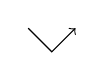
\begin{tikzpicture}[xscale=0.3, yscale=0.3, baseline=(O)]
		\coordinate (O) at (0, -0.8);
		\draw[->] (0,0) -- (1, -1) -- (2, 0);
	\end{tikzpicture}$
	部分确定. 然而 $Y \xrightarrow{c_k} M_k \xleftarrow{t_k} X_k$ 给出 $f_k$. 对照此前对 $f$ 的构造, 可见 $f = g$. 证毕.
\end{proof}

\begin{remark}
	若将积 (或余积) 的下标集换成任意小集 $I$, 仍有相应的陈述.
\end{remark}

命 $\mathcal{D}$ 为 $\cate{Ab}$-范畴. 考虑 \eqref{eqn:InvSys} 定义的范畴 $\cate{InvSys}(\mathcal{D}) := \mathcal{D}^{\Z_{\geq 0}^{\opp}}$, 其对象即资料 $X = (X_k, f_k)_{k \geq 0}$, 其中 $X_k \in \Obj(\mathcal{D})$ 而 $f_k \in \Hom_{\mathcal{D}}(X_{k+1}, X_k)$. 若 $\mathcal{D}$ 有可数积, 按定义 \ref{def:Delta-diff} 的方式定义典范态射
\[ \Delta_X := T_X - \identity: \prod_k X_k \to \prod_k X_k. \]
\index[sym1]{InvSys}
\index[sym1]{DirSys@$\cate{DirSys}$}

对偶地, 范畴 $\cate{DirSys}(\mathcal{D}) := \mathcal{D}^{\Z_{\geq 0}}$ 的对象即资料\footnote{又称为 $\mathcal{D}$ 中的正向系.} $X = (X_k, g_k)_{k \geq 0}$, 其中 $X_k \in \Obj(\mathcal{D})$ 而 $g_k \in \Hom_{\mathcal{D}}(X_k, X_{k+1})$. 以同样手法定义 $\nabla_X := T_X - \identity : \bigoplus_k X_k \to \bigoplus_k X_k$, 前提是 $\mathcal{D}$ 有可数余积; $T_X$ 仍是类似的平移态射.

假使 $\Ker(\Delta_X)$ 或 $\Coker(\nabla_X)$ 存在, 则有典范同构
\begin{align*}
	X \in \Obj\left( \cate{InvSys}(\mathcal{D}) \right) & \implies \varprojlim_k X_k \simeq \Ker(\Delta_X), \\
	X \in \Obj\left( \cate{DirSys}(\mathcal{D}) \right) & \implies \varinjlim_k X_k \simeq \Coker(\nabla_X).
\end{align*}
朴素的愿望是施此于 $\mathcal{D} = \cate{D}(\mathcal{A})$. 导出范畴鲜少是 Abel 范畴. 尽管如此, 注记 \ref{rem:homotopy-kernel-cokernel} 说明映射锥可充当核与余核的某种同伦版本; 三角范畴中粗略对应的构造是好三角.

\begin{definition}[M.\ Bökstedt, A.\ Neeman {\cite{BN93}}]\label{def:holim}
	\index{tonglunjixian@同伦极限, 同伦余极限 (homotopy limit, homotopy colimit)}
	\index[sym1]{holim@$\holim$, $\hocolim$}
	设 $\mathcal{D}$ 是三角范畴.
	\begin{itemize}
		\item 若 $\mathcal{D}$ 有可数积, 则 $\cate{InvSys}(\mathcal{D})$ 的对象 $X$ 的\emph{同伦极限} (或称同伦 $\varprojlim$) 意谓 $\mathcal{D}$ 的好三角
		\[ \holim(X) \to \prod_k X_k \xrightarrow{\Delta_X} \prod_k X_k \xrightarrow{+1} . \]
		\item 若 $\mathcal{D}$ 有可数余积, 则 $\cate{DirSys}(\mathcal{D})$ 的对象 $X$ 的\emph{同伦余极限} (或称同伦 $\varinjlim$) 意谓 $\mathcal{D}$ 的好三角
		\[ \bigoplus_k X_k \xrightarrow{\nabla_X} \bigoplus_k X_k \to \hocolim(X) \xrightarrow{+1} . \]
	\end{itemize}
\end{definition}

上述定义涉及的好三角彼此同构 (推论 \ref{prop:Cone-uniqueness}), 但同构非典范.

回到复形的讨论. 留意到 $\cate{InvSys}\left(\cate{C}(\mathcal{A})\right) = \cate{C}(\cate{InvSys}(\mathcal{A}))$, 两者的对象 $X$ 同为交换图表
\[\begin{tikzcd}
	& \vdots \arrow[d, "{f_1^n}"'] & \vdots \arrow[d, "{f_1^{n+1}}"] & \\
	\cdots \arrow[r] & X_1^n \arrow[r, "{d_{X_1}^n}"] \arrow[d, "{f_0^n}"'] & X_1^{n+1} \arrow[d, "{f_0^{n+1}}"] \arrow[r] & \cdots \\
	\cdots \arrow[r] & X_0^n \arrow[r, "{d_{X_0}^n}"] & X_0^{n+1} \arrow[r] & \cdots
\end{tikzcd} \quad \text{每行皆为复形}; \]
其间的态射同为双层交换图表. 依此遂可在 $\mathcal{D} := \cate{D}(\mathcal{A})$ 中比较 $\holim(X)$ 和 $\varprojlim$ 的右导出函子 $\mathrm{R}\lim(X)$, 前提是它们存在.

也留意到对 $\cate{C}(\cate{InvSys}(\mathcal{A}))$ 的对象 $X$ 取上同调 $\Hm^m$, 产物是 $\left(\Hm^m(X_k), \Hm^m(f_k)\right)_{k \geq 0}$. 所以 $X \to Y$ 是拟同构等价于每个 $X_k \to Y_k$ 都是 $\cate{C}(\mathcal{A})$ 中的拟同构.

\begin{theorem}\label{prop:Rlim-as-holim}
	设 $\mathcal{A}$ 为 Abel 范畴, 具有正合的可数积和足够的内射对象.
	\begin{enumerate}[(i)]
		\item 左正合函子 $\varprojlim: \cate{InvSys}(\mathcal{A}) \to \mathcal{A}$ 的右导出函子存在, 记为
		\[ \mathrm{R}\lim :  \cate{D}^+\left(\cate{InvSys}(\mathcal{A})\right) \to \cate{D}^+(\mathcal{A}) . \]
		\item 对 $\cate{C}^+(\cate{InvSys}(\mathcal{A}))$ 的任意对象 $X = (X_k, f_k)_{k \geq 0}$, 在 $\cate{D}(\mathcal{A})$ 中存在好三角
		\[ \mathrm{R}\lim(X) \to \prod_k X_k \xrightarrow{\Delta_X} \prod_k X_k \xrightarrow{+1} \]
		特别地, $\mathrm{R}\lim(X) \simeq \holim(X)$.
		\item 在定义--命题 \ref{def:dim-functor} 的意义下, $\mathrm{R}\lim$ 的维数 $\leq 1$.
	\end{enumerate}
\end{theorem}
\begin{proof}
	因为 $\cate{InvSys}(\mathcal{A})$ 有足够的内射对象, 故 (i) 成立. 更精确地说, 取引理 \ref{prop:lim1-prep} 的范畴 $\mathcal{R}$, 将 $\cate{InvSys}(\mathcal{A})$ 和 $\mathcal{R}$ 代入定理 \ref{prop:resolution-existence}, 可知对 $\cate{C}^+(\cate{InvSys}(\mathcal{A}))$ 的任意对象 $X = (X_k, f_k)_{k \geq 0}$, 存在拟同构 $X \to Y$ 使得 $Y \in \Obj\left( \cate{C}^+(\mathcal{R}) \right)$. 于是 $\mathrm{R}\lim(X) = \varprojlim Y$. 而 $\mathcal{R}$ 的定义又确保 $\Delta_Y$ 逐次满, 故有 $\cate{C}^+(\mathcal{A})$ 的短正合列
	\[ 0 \to \varprojlim Y \to \prod_{k \geq 0} Y_k \xrightarrow{\Delta_Y} \prod_{k \geq 0} Y_k \to 0. \]
	其次, $X_k \to Y_k$ 对每个 $k$ 皆是拟同构, 故 $\prod_{k \geq 0} X_k \to \prod_{k \geq 0} Y_k$ 也是拟同构. 这便给出 (ii) 断言的好三角
	\[ \mathrm{R}\lim(X) \to \prod_{k \geq 0} X_k \xrightarrow{\Delta_X} \prod_{k \geq 0} X_k \xrightarrow{+1} . \]

	至于 (iii), 注意到当 $X \in \Obj(\cate{InvSys}(\mathcal{A}))$ 时 $\Delta_X$ 简化为 $\cate{InvSys}(\mathcal{A})$ 的态射, 而 $\holim(X) \simeq \Cone(\Delta_X)[-1]$ 是 $\cate{D}^{[0,1]}(\mathcal{A})$ 的对象; 当然这也是定理 \ref{prop:lim1} 的复述. 
\end{proof}

对于 $\varinjlim: \cate{DirSys}(\mathcal{A}) \to \mathcal{A}$, 定理 \ref{prop:Rlim-as-holim} 有对偶版本, 不再赘述.

例 \ref{eg:Rlim-unbounded} 将说明如何对无界导出范畴得到 $\mathrm{R}\lim$, 使得定理 \ref{prop:Rlim-as-holim} (ii) 依然适用.

\section{无界导出函子}\label{sec:unbounded-derived}
\index{daochuhanzi!无界 (unbounded)}
考虑 Abel 范畴之间的加性函子 $F: \mathcal{A} \to \mathcal{A}'$. 本节回到定义 \ref{def:derived-functor}, 着重探讨无界导出范畴版本的导出函子
\[ \mathrm{R}F, \; \mathrm{L}F: \cate{D}(\mathcal{A}) \to \cate{D}(\mathcal{A}'). \]

为了确保 $\mathrm{R}F$ 或 $\mathrm{L}F$ 存在并进行操作, 需要定义 \ref{def:K-resolutions} 的 K-内射复形或 K-投射复形, 以及相应的解消等概念.

\begin{lemma}\label{prop:K-injective-zero}
	设 $\mathcal{A}$ 为 Abel 范畴. 设 $Z \in \Obj(\cate{K}(\mathcal{A}))$ 既是 K-内射 (或 K-投射) 又是零调的, 则 $Z = 0$.
\end{lemma}
\begin{proof}
	引理 \ref{prop:K-injective-criterion} 蕴涵 $\Hom_{\cate{K}(\mathcal{A})}(Z, Z) = 0$.
\end{proof}

兹陈述一则一般结果. 选定三角范畴 $\mathcal{D}_1, \mathcal{D}_2, \mathcal{D}'$ 及其饱和子三角范畴 $\mathcal{N}_1, \mathcal{N}_2, \mathcal{N}'$.

\begin{lemma}\label{prop:K-cats}
	给定三角双函子 $G: \mathcal{D}_1 \times \mathcal{D}_2 \to \mathcal{D}'$, 定义 $\mathcal{D}_2$ 的全子范畴 $\mathcal{K}_2^G$ 使得
	\[ \Obj(\mathcal{K}_2^G) = \left\{ X_2 \in \Obj(\mathcal{D}_2) : X_1 \in \Obj(\mathcal{N}_1) \implies G(X_1, X_2) \in \Obj(\mathcal{N}') \right\}, \]
	则 $\mathcal{K}_2^G$ 是饱和子三角范畴. 如将变元位置调换, 相应的叙述对 $\mathcal{K}_1^G \subset \mathcal{D}_1$ 依然成立.
\end{lemma}
\begin{proof}
	由 $G(X_1, X_2[1]) \simeq G(X_1, X_2)[1]$ 可知 $\mathcal{K}_2^G$ 对平移封闭. 同理, 设有好三角 $I \to J \to K \xrightarrow{+1}$, 其中 $I, K \in \Obj(\mathcal{K}_2^G)$, 则从好三角
	\[ G(X_1, I) \to G(X_1, J) \to G(X_1, K) \xrightarrow{+1} \]
	容易看出 $X_1 \in \Obj(\mathcal{N}_1) \implies G(X_1, J) \in \Obj(\mathcal{N}')$. 饱和性质是自明的.
\end{proof}

此结果可以应用于 $\Hom: \mathcal{A}^{\opp} \times \mathcal{A} \to \cate{Ab}$ 以及相应的三角双函子 $\cate{K}_{\Pi}\Hom$. 例 \ref{eg:Hom-bicplx} 已经说明后者本质上即是 $\Hom$ 复形:
\begin{equation}\label{eqn:CPiHom}\begin{gathered}
	(\cate{C}_{\Pi} \Hom)(\sigma^{-1} X_1, X_2) \simeq \Hom^\bullet\left( X_1, X_2 \right), \\
	(\cate{K}_\Pi \Hom)(\sigma^{-1} X_1, X_2) \simeq \Hom^\bullet\left( X_1, X_2 \right)\; \text{在 $\cate{K}(\cate{Ab})$ 中的像},
\end{gathered}\end{equation}
其中 $\sigma: \cate{C}(\mathcal{A}^{\opp}) \rightiso \cate{C}(\mathcal{A})^{\opp}$ 和 $\cate{K}(\mathcal{A}^{\opp}) \rightiso \cate{K}(\mathcal{A})^{\opp}$ 如定义--命题 \ref{def:sigma} 和命题 \ref{prop:sigma-homotopy}. 稍后将需要它的导出范畴版本.

\begin{proposition}\label{prop:K-injective-F-injective}
	全体 K-内射复形 (或 K-投射复形) 构成 $\cate{K}(\mathcal{A})$ 的饱和子三角范畴 $\mathcal{I}$ (或 $\mathcal{P}$). 若 $\mathcal{A}$ 有足够的 K-内射 (或 K-投射) 复形, 则 $\mathcal{I}$ (或 $\mathcal{P}$) 对任意加性函子 $F: \mathcal{A} \to \mathcal{A}'$ 都是 $F$-内射的 (或 $F$-投射的).
\end{proposition}
\begin{proof}
	仅论 K-内射情形. 前半部是配合 K-内射复形的定义 \ref{def:K-resolutions} 和 \eqref{eqn:CPiHom}, 将引理 \ref{prop:K-cats} 施于 $G = \cate{K}_{\Pi}\Hom$ 的结果: 该处的 $\mathcal{K}_2^G$ 正是此处的 $\mathcal{I}$.
	
	设 $\mathcal{A}$ 有足够的 K-内射复形. 若 $I$ 是零调 K-内射复形, 则引理 \ref{prop:K-injective-zero} 蕴涵 $I = 0$, 故 $(\cate{K}F)I$ 当然零调. 因此定义 \ref{def:F-injective} 对 $F$-内射子三角范畴的全部条件成立.
\end{proof}

命 $Q: \cate{K}(\mathcal{A}) \to \cate{D}(\mathcal{A})$ 和 $Q': \cate{K}(\mathcal{A}') \to \cate{D}(\mathcal{A}')$ 为局部化函子.

\begin{corollary}
	若 $\mathcal{A}$ 有足够的 K-内射复形, 则 $F$ 有右导出函子 $\mathrm{R}F: \cate{D}(\mathcal{A}) \to \cate{D}(\mathcal{A}')$, 使得当 $X$ 为 K-内射复形时 $\mathrm{R}F(QX) \simeq Q' \cate{K}F(X)$.
	
	对偶地, 若 $\mathcal{A}$ 有足够的 K-投射复形, 则 $F$ 有左导出函子 $\mathrm{L}F: \cate{D}(\mathcal{A}) \to \cate{D}(\mathcal{A}')$, 使得当 $X$ 为 K-投射复形时 $\mathrm{L}F(QX) \simeq Q' \cate{K}F(X)$.
\end{corollary}
\begin{proof}
	将命题 \ref{prop:K-injective-F-injective} 的结论代入命题 \ref{prop:localization-injective} 的一般框架.
\end{proof}

现在选定 Abel 范畴 $\mathcal{A}_1$, $\mathcal{A}_2$, $\mathcal{B}$. 对加性双函子 $F: \mathcal{A}_1 \times \mathcal{A}_2 \to \mathcal{B}$ 考虑定义 \ref{def:derived-bifunctor} 的导出双函子 $\mathrm{R}F$ (或 $\mathrm{L}F$) 的无界版本; 以下皆假设 $\mathcal{B}$ 有可数积 (或可数余积).

具体地说, 我们希望以上述子范畴 $\mathcal{I}_1$, $\mathcal{I}_2$ (或 $\mathcal{P}_1$, $\mathcal{P}_2$) 确定 $\mathrm{R}F$ (或 $\mathrm{L}F$).

\begin{lemma}\label{prop:bifunctor-via-K-injective-prep}
	取 $\cate{K}(\mathcal{A}_i)$ 的子三角范畴 $\mathcal{I}_i$ (或 $\mathcal{P}_i$) 如命题 \ref{prop:K-injective-F-injective}, 其中 $i=1, 2$.
	\begin{compactitem}
		\item 若 $\mathcal{A}_1$ 和 $\mathcal{A}_2$ 有足够的 K-内射复形, 则 $\mathcal{I}_1 \times \mathcal{I}_2$ 是 $F$-内射的.
		\item 若 $\mathcal{A}_1$ 和 $\mathcal{A}_2$ 有足够的 K-投射复形, 则 $\mathcal{P}_1 \times \mathcal{P}_2$ 是 $F$-投射的.
	\end{compactitem}
\end{lemma}
\begin{proof}
	仅论 K-内射情形. 关键在于说明若 $X_1 \in \Obj(\mathcal{I}_1)$, 则 $(\cate{K}_{\Pi} F)(X_1, \cdot)$ 映 $\mathcal{I}_2$ 的所有零调对象 $Z$ 为 $\cate{K}(\mathcal{B})$ 的零调对象. 但引理 \ref{prop:K-injective-zero} 说明 $Z=0$, 而 $(\cate{K}_{\Pi} F)(X_1, \cdot)$ 是加性函子, 故这是当然的. 下标 $1, 2$ 调换后也有相应的结果.
\end{proof}

命 $Q: \cate{K}(\mathcal{B}) \to \cate{D}(\mathcal{B})$ 和 $Q_i: \cate{K}(\mathcal{A}_i) \to \cate{D}(\mathcal{A}_i)$ 为局部化函子 ($i=1,2$).

\begin{proposition}\label{prop:bifunctor-via-K-injective}
	给定 $F: \mathcal{A}_1 \times \mathcal{A}_2 \to \mathcal{B}$, 设 $\mathcal{A}_1$ 和 $\mathcal{A}_2$ 皆有足够的 K-内射 (或 K-投射) 复形, 则导出双函子 $\mathrm{R}F$ (或 $\mathrm{L}F$) 存在. 若 $X_i \in \Obj(\cate{K}(\mathcal{A}))$ 对 $i=1, 2$ 都是 K-内射的 (或 K-投射的), 则有典范同构
	\[ \mathrm{R}F(Q_1 X_1, Q_2 X_2) \simeq Q (\cate{K}_{\Pi} F)(X_1, X_2) \quad \text{(或 $\mathrm{L}F(Q_1 X_1, Q_2 X_2) \simeq Q (\cate{K}_{\oplus} F)(X_1, X_2)$) }. \]
\end{proposition}
\begin{proof}
	直接将引理 \ref{prop:bifunctor-via-K-injective-prep} 的结果代入命题 \ref{prop:localization-injective-bifunctor}.
\end{proof}

对于具体给定的双函子 $F$, 经常可以取到比 K-内射 (或 K-投射) 复形更大的 $F$-内射 (或 $F$-投射) 子三角范畴. 以下着重讨论的 $\RHom$ 即是一例.

\begin{theorem}[无界 $\RHom$]\label{prop:unbounded-RHom}
	\index{RHom hanzi}
	\index[sym1]{RHom}
	设 Abel 范畴 $\mathcal{A}$ 有足够的 K-内射复形, 或足够的 K-投射复形. 将局部化函子统一记为 $Q$ 以简化符号.
	\begin{enumerate}[(i)]
		\item 双函子 $\Hom = \Hom_{\mathcal{A}}: \mathcal{A}^{\opp} \times \mathcal{A} \to \cate{Ab}$ 有右导出函子 $\cate{D}(\mathcal{A}^{\opp}) \times \cate{D}(\mathcal{A}) \to \cate{D}(\cate{Ab})$, 它也可以通过命题 \ref{prop:derived-cat-op} 的等价 $\sigma$ 写作
		\[ \RHom: \cate{D}(\mathcal{A})^{\opp} \times \cate{D}(\mathcal{A}) \to \cate{D}(\cate{Ab}). \]
		事实上, 若 $\mathcal{A}$ 有足够的 K-内射 (或 K-投射) 复形, 则 $\cate{K}(\mathcal{A})^{\opp} \times \mathcal{I}$ (或 $\mathcal{P}^{\opp} \times \cate{K}(\mathcal{A})$) 是 $\Hom$-内射的.
		\item 设 $\mathcal{A}$ 有足够的 K-内射复形, $X_2 \to I_2$ 是 K-内射解消, 则它诱导
		\[ \RHom(Q X_1, Q X_2) \rightiso Q \Hom^\bullet(X_1, I_2). \]
		作为特例, $\RHom(Q X_1, \cdot) \simeq \mathrm{R}\left( \Hom(X_1, \cdot) \right)$.
		\item 设 $\mathcal{A}$ 有足够的 K-投射复形, $P_1 \to X_1$ 是 K-投射解消, 则它诱导
		\[ \RHom(Q X_1, Q X_2) \rightiso Q \Hom^\bullet(P_1, X_2). \]
		作为特例, $\RHom(\cdot, Q X_2) \simeq \mathrm{R}\left(\Hom(\cdot, X_2)\right)$.
		\item 存在典范同构 $\Hm^n \RHom(X, Y) \simeq \Hom_{\cate{D}(\mathcal{A})}(X, Y[n]) =: \Ext^n(X, Y)$ (定义 \ref{def:Ext-general}).
	\end{enumerate}
\end{theorem}
\begin{proof}
	和定理 \ref{prop:RHom-bounded} 几乎平行. 以 $\mathcal{A}$ 有足够的 K-内射复形的情形为例, 关键在于说明 $\cate{K}(\mathcal{A})^{\opp} \times \mathcal{I}$ 是 $\Hom$-内射的.
	\begin{itemize}
		\item 固定复形 $X_1$, 函子 $(\cate{K}_\Pi \Hom)(X_1, \cdot)$ 映一切零调 K-内射复形 $X_2$ 为零调复形, 这是因为 $X_2$ 在 $\cate{K}(\mathcal{A})$ 中为 $0$ (引理 \ref{prop:K-injective-zero}).
		\item 固定 K-内射复形 $X_2$, 设复形 $X_1$ 零调, 则 K-内射复形的定义导致 $\Hom^\bullet\left( X_1, X_2 \right)$ 零调, 代入 \eqref{eqn:CPiHom} 可见 $(\cate{K}_\Pi \Hom)(X_1, X_2)$ 也零调.
	\end{itemize}
	这便验证了 $\Hom$-内射所需的零调条件, 而解消条件是平凡的.
\end{proof}

\begin{theorem}\label{prop:RHom-adjoint}
	考虑 Abel 范畴之间的一对伴随加性函子
	$\begin{tikzcd}
		F: \mathcal{A} \arrow[r, shift left] & \mathcal{A}' \arrow[l, shift left] : G
	\end{tikzcd}$.
	设 $\mathcal{A}$ 有足够的 K-投射复形, $\mathcal{A}'$ 有足够的 K-内射复形. 此时存在 $\cate{D}(\cate{Ab})$ 中的典范同构
	\[ \RHom_{\mathcal{A'}}\left(\mathrm{L}F(X), Y\right) \simeq \RHom_{\mathcal{A}}\left(X, \mathrm{R}G(Y) \right), \]
	其中 $X \in \Obj\left(\cate{D}(\mathcal{A})\right)$, $Y \in \Obj\left(\cate{D}(\mathcal{A}')\right)$.
\end{theorem}
\begin{proof}
	论证和定理 \ref{prop:RHom-adjoint-bounded} 相同. 唯一差别在于以 K-内射 (或 K-投射) 解消代替内射 (或投射) 解消, 并且以定理 \ref{prop:K-resolution-homotopy} 代替定理 \ref{prop:resolution-homotopy} 来探讨解消的唯一性.
\end{proof}

\begin{remark}
	对定理 \ref{prop:RHom-adjoint} 两边同取 $\Hm^0$, 即有伴随关系
	\[ \Hom_{\cate{D}(\mathcal{A'})}\left(\mathrm{L}F(X), Y\right) \simeq \Hom_{\cate{D}(\mathcal{A})}\left(X, \mathrm{R}G(Y) \right). \]

	由于通过解消得到的导出函子总是定义 \ref{def:absolute-Kan} 的绝对 Kan 延拓 (命题 \ref{prop:localization-functor-abs}), 定理 \ref{prop:Quillen-adjunction-gen} 也断言 $(\mathrm{L}F, \mathrm{R}G)$ 是伴随对. 两者给出相同的伴随同构. 何以故? 问题化约到 $X$ 是 K-投射复形而 $Y$ 是 K-内射复形的情形, 此时定理 \ref{prop:RHom-adjoint} 的伴随同构通过 $\cate{K}(\cdot)$ 层次的单位 $\eta$ 和余单位 $\varepsilon$ 具体实现为
	\begin{align*}
		\Hom_{\cate{K}(\mathcal{A}')}\left( \cate{K}F(X), Y\right) \simeq \Hom_{\cate{K}(\mathcal{A})}\left( X, \cate{K}G(Y) \right).
	\end{align*}
	另一方面, 定理 \ref{prop:Quillen-adjunction-gen} 在导出范畴层次确定了 $\underline{\eta}$ 和 $\underline{\varepsilon}$, 该处给出的刻画足以说明它们和 $\eta$, $\varepsilon$ 相容. 细节请感兴趣的读者琢磨.
\end{remark}

最后, 得到无界导出函子的另一套充分条件是基于维数的有限性 (定义--命题 \ref{def:dim-functor}). 虽然其证明技术不超出本书范围, 为了避免岔题, 权且述而不证. 详见 {\cite[Tags 07K6, 07K7]{stacks}}. 我们的起点是定理 \ref{prop:derived-via-resolution} 对有界导出函子的构造.

\begin{proposition}\label{prop:unbounded-derived-fd}
	\index{weishu}
	取 $F: \mathcal{A} \to \mathcal{A}'$ 为 Abel 范畴之间的左正合 (或右正合) 函子. 假设
	\begin{compactitem}
		\item 相对于 $F$, 存在 $\mathcal{A}$ 的 I 型 (或 P 型) 加性全子范畴 $\mathcal{A}^\flat$, 如定义--命题 \ref{prop:F-injective-criterion};
		\item 相应的有界导出函子 ${}^+ \mathrm{R}F$ (或 ${}^- \mathrm{L}F$) 维数有限.
	\end{compactitem}
	此时 $\mathrm{R}F$ (或 $\cate{L}F$): $\cate{D}(\mathcal{A}) \to \cate{D}(\mathcal{A}')$ 存在; 事实上, $\cate{K}(\mathcal{A}^\flat)$ 构成 $\cate{K}(\mathcal{A})$ 的 $F$-内射 (或 $F$-投射) 子范畴.
\end{proposition}

\begin{example}\label{eg:Rlim-unbounded}
	设 $\mathcal{A}$ 具有正合的可数积和足够的内射对象. 取左正合函子 $F$ 为 $\varprojlim: \cate{InvSys}(\mathcal{A}) \to \mathcal{A}$. 定理 \ref{prop:Rlim-as-holim} (iii) 说明有界版本 $\mathrm{R}\lim$ 的维数 $\leq 1$, 子范畴 $\mathcal{R} \subset \cate{InvSys}(\mathcal{A})$ 对之是 I 型的. 前述结果因而给出无界导出函子
	\[ \mathrm{R}\lim: \cate{D}(\cate{InvSys}(\mathcal{A})) \to \cate{D}(\mathcal{A}). \]
	
	一如定理 \ref{prop:Rlim-as-holim} (ii) 的情形, 对 $\cate{C}(\cate{InvSys}(\mathcal{A}))$ 的所有对象 $X$ 皆有 $\cate{D}(\mathcal{A})$ 的好三角
	\[ \mathrm{R}\lim(X) \to \prod_k X_k \xrightarrow{\Delta_X} \prod_k X_k \xrightarrow{+1} . \]
	特别地, $\mathrm{R}\lim(X) \simeq \holim(X)$. 基于命题 \ref{prop:unbounded-derived-fd} 的结论, 原证明可以照搬: 将一切 $\cate{C}^+(\cdots)$ 直接改为 $\cate{C}(\cdots)$ 便是.
\end{example}

\section{实例: K-平坦复形和 \texorpdfstring{$\otimesL$}{otimesL}}\label{sec:otimesL}
本节选定交换环 $\Bbbk$.

\begin{convention}\label{con:bimodule-algebra}
	设 $R$, $S$ 为 $\Bbbk$-代数, 按本书惯例, $(R,S)$-双模 $M$ 默认满足 $tm = mt$, 其中 $t \in \Bbbk$ 而 $m \in M$. 换言之 $(R,S)\dcate{Mod} \simeq (R \dotimes{\Bbbk} S^{\opp})\dcate{Mod}$. 当 $\Bbbk = \Z$ 时, 此条件是多余的.
	
	今后将忘却函子 $(R,S)\dcate{Mod} \to R\dcate{Mod}$ (或 $(R,S)\dcate{Mod} \to \cated{Mod}S$) 记为 $M \mapsto {}_R M$ (或 $M \mapsto M_S$); 同样记法适用于复形. 忘却函子是正合的, 它们在导出范畴之间诱导的三角函子也按相同方式标记.
\end{convention}

一则平凡的观察: 对于任何由 $(R, S)$-双模构成的复形 $M$, 我们有
\[ M_S \;\text{零调} \iff M \;\text{零调} \iff {}_R M \;\text{零调}. \]

今后设 $R$, $A$, $B$ 为 $\Bbbk$-代数. 我们的出发点是张量积给出的双函子
\[ \otimes_R: (A, R)\dcate{Mod} \times (R, B)\dcate{Mod} \to (A, B)\dcate{Mod}, \]
它对每个变元都右正合. 最单纯的是 $A = \Bbbk = B$ 的情形, 对应的双函子化为 $\otimes_R: \cated{Mod}R \times R\dcate{Mod} \to \cate{\Bbbk}$.

简单起见, 对于 $(A,R)$-双模构成的复形 $X$ 和 $(R,B)$-双模构成的复形 $Y$, 今后将逐项作张量积得到的双复形记为 $X^\bullet \dotimes{R} Y^\bullet$, 而将其全复形记为
\[ X \dotimes{R} Y := \tot_{\oplus} \left( X^\bullet \dotimes{R} Y^\bullet \right). \]

双模范畴有足够的 K-投射复形 (应用例 \ref{eg:Mod-K-injectives}), 故命题 \ref{prop:bifunctor-via-K-injective} 确保无界左导出双函子存在.

\begin{definition}\label{def:otimesL}
	\index{daochuzhangliangji@导出张量积 (derived tensor product)}
	\index[sym1]{XotimesLY@$X \otimesL[R] Y$}
	记 $\otimes_R$ 的左导出函子 $\mathrm{L}\left( \cdot \dotimes{R} \cdot \right)$ 为
	\[ \otimesL[R] : \cate{D}((A, R)\dcate{Mod}) \times \cate{D}((R, B)\dcate{Mod}) \to \cate{D}((A, B)\dcate{Mod}). \]
	不致混淆时, 也将 $X \otimesL[R] Y$ 简记为 $X \otimesL Y$.
\end{definition}

上述抽象定义直截了当, 但仍须引入称为 K-平坦解消的一类拟同构来助推 $\otimes_R$ 的研究, 理由包括:
\begin{itemize}
	\item K-平坦解消的定义与张量积直接相关, 而且对于确立一些重要性质和实际计算更有意义, 这点在 \S\ref{sec:Ext-Tor} 已有体现;
	\item 在层论等几何场景中, 可能仅有 K-内射解消而无 K-投射解消, 此时 K-平坦解消是研究导出张量积的唯一手段.
\end{itemize}

\begin{definition}[N.\ Spaltenstein {\cite[Definition 5.1]{Spa88}}]
	\index{fuxing!K-平坦 (K-flat)}
	设 $X$ 为右 $R$-模构成的复形. 若对所有由左 $R$-模构成的复形 $Y$,
	\[ Y \;\text{零调} \implies X \dotimes{R} Y\;\text{零调}, \]
	则称 $X$ 是 \emph{K-平坦}的\footnote{更合理的名称兴许是同伦平坦复形.}; 此性质仅关乎 $X$ 在 $\cate{K}(\cated{Mod}R)$ 中的同构类. 类似手法可对左 $R$-模构成的复形定义何谓 K-平坦.
\end{definition}

对于上有界复形, K-平坦性可归结为模论中熟知的平坦性.

\begin{proposition}\label{prop:flat-K-flat}
	设 $X$ 为 $\cate{C}^-(\cated{Mod}R)$ 的对象, 而且每个 $X^n$ 皆平坦, 则 $X$ 是 K-平坦的. 对  $\cate{C}^-(R\dcate{Mod})$ 的对象亦同.
\end{proposition}
\begin{proof}
	设 $Y$ 为左 $R$-模构成的零调复形, 今将往证 $X \dotimes{R} Y$ 零调. 应用截断函子将 $Y$ 表为 $\varinjlim_m \tau^{\leq m} Y$. 逐次地看, $\varinjlim_m$ 既和张量积交换 \cite[命题 6.9.2]{Li1}, 又和 $\bigoplus$ 交换, 问题因此化到 $Y$ 上有界的情形. 于是 $X^\bullet \dotimes{R} Y^\bullet$ 落在定义 \ref{def:Cf-Supp} 的范畴 $\cate{C}^2_f(\Bbbk\dcate{Mod})$. 因为 $X^p \dotimes{R} Y^\bullet$ 对每个 $p$ 皆零调, 推论 \ref{prop:acyclic-assembly} 确保 $X \dotimes{R} Y$ 零调.
\end{proof}

有鉴于此, 倘若读者只关心上有界导出范畴, 则不妨将本节出现的所有 K-平坦复形都代换为由平坦模构成的上有界复形.

\begin{definition}
	\index{jiexiao!K-平坦 (K-flat)}
	\index{zugoude K-pingtan fuxing@足够的 K-平坦复形 (enough K-flats)}
	若 $P \to X$ 是 $\cate{C}((A,R)\dcate{Mod})$ 中的拟同构, 而且 $P_R$ 是 K-平坦的, 则称之为 $X$ 对 $R$ 的 \emph{K-平坦解消}. 如果所有 $X \in \cate{C}((A, R)\dcate{Mod})$ 都有对 $R$ 的 K-平坦解消, 则称 $(A, R)\dcate{Mod}$ 对 $R$ 有足够的 K-平坦复形.
	
	以类似手法定义 $X \in \Obj(\cate{C}((R, B)\dcate{Mod}))$ 对 $R$ 的 K-平坦解消.
\end{definition}

我们自然要问: 如何确保双模范畴对 $R$ 有足够的 K-平坦复形? K-平坦和 K-投射复形之间有何关系? 毫不意外, 桥梁来自 $\otimes$ 和 $\Hom$ 之间经典的伴随关系 \cite[定理 6.6.5]{Li1}.

为此, 首务是将伴随关系升级到复形层次. 若 $Y$ 为 $\cate{C}((R, B)\dcate{Mod})$ 的对象, $Z$ 为 $\cate{C}((A, B)\dcate{Mod})$ 的对象, 则 $\Hom$ 复形 $\Hom^\bullet(Y_B, Z_B)$ 可逐次地赋予 $(A, R)$-双模结构, 这给出 $\cate{C}((A, R)\dcate{Mod})$ 的对象.

\begin{proposition}[$\Hom$ 和 $\otimes$ 的伴随关系: 复形版本]\label{prop:tensor-Hom-cplx}
	设 $X$ 为 $\cate{C}((A, R)\dcate{Mod})$ 的对象, $Y$ 为 $\cate{C}((R, B)\dcate{Mod})$ 的对象, $Z$ 为 $\cate{C}((A, B)\dcate{Mod})$ 的对象. 存在 $\cate{C}(\Bbbk\dcate{Mod})$ 中的典范同构
	\begin{align*}
		\Hom^\bullet\left( X \dotimes{R} Y, \; Z \right) & \simeq \Hom^\bullet\left( X, \Hom^\bullet(Y_B, Z_B) \right) \\
		& \simeq \Hom^\bullet\left( Y, \Hom^\bullet({}_A X, {}_A Z) \right).
	\end{align*}

	作为推论, 取 $\Ker(d^0)$ 便有 $\Bbbk$-模的同构
	\begin{align*}
		\Hom_{\cate{C}((A, B)\dcate{Mod})}\left( X \dotimes{R} Y, \; Z \right) & \simeq \Hom_{\cate{C}((A, R)\dcate{Mod})}\left( X, \Hom^\bullet(Y_B, Z_B) \right) \\
		& \simeq \Hom_{\cate{C}((R, B)\dcate{Mod})}\left( Y, \Hom^\bullet({}_A X, {}_A Z) \right).
	\end{align*}
\end{proposition}
\begin{proof}
	处理第一个同构即可. 为简化计, 以下将 $Y_B$ 和 $Z_B$ 直接记为 $Y$ 和 $Z$, 同时省略 $\Hom$ 的下标. 选定 $n \in \Z$. 同构左侧的 $n$ 次项是
	\begin{multline}\label{eqn:tensor-Hom-cplx-aux}
		\prod_k \Hom\left( (X \dotimes{R} Y)^k, Z^{k+n}\right) \simeq \prod_k \prod_{p+q=k} \Hom\left(X^p \dotimes{R} Y^q, Z^{k+n}\right) \\
		= \prod_{p, q} \Hom\left( X^p \dotimes{R} Y^q, Z^{p+q+n} \right) \simeq \prod_p \prod_q \Hom\left( X^p, \Hom\left(Y^q, Z^{p+q+n}\right) \right) \\
		\simeq \prod_p \Hom\left( X^p, \Hom^{p+n}(Y, Z) \right),
	\end{multline}
	末项即同构右侧的 $n$ 次项. 具体地说, $(A, B)$-双模同态 $\varphi^{p, q}: X^p \dotimes{R} Y^q \to Z^{p+q+n}$ 在第二个 $\simeq$ 之下对应
	\[ \left[ x \mapsto [y \mapsto \varphi^{p,q}(x \otimes y)] \right] \; \in \Hom\left( X^p, \Hom\left(Y^q, Z^{p+q+n}\right) \right). \]
	后续工作只剩下验证 \eqref{eqn:tensor-Hom-cplx-aux} 确定复形的同构.
	
	给定左侧的 $n$ 次项元素, 表作 $(\varphi^{p,q})_{p, q \in \Z}$, 它对 $d_{\Hom^\bullet(X \otimes Y, Z)}$ 的像的 $(p, q)$ 分量映 $x \otimes y \in X^p \dotimes{R} Y^q$ 为
	\[ d_Z \varphi^{p,q}(x \otimes y) - (-1)^n \left( \varphi^{p+1, q}(d_X x \otimes y) + (-1)^p \varphi^{p, q+1}(x \otimes d_Y y) \right). \]
	
	对于右侧相应的 $n$ 次项元素, 它对 $d_{\Hom^\bullet(X, \Hom^\bullet(Y, Z))}$ 的像的 $p$ 分量映 $x \in X^p$ 为
	\[
		d_{\Hom^\bullet(Y, Z)}\left[ y \mapsto \varphi^{p,q}(x \otimes y) \right]_{q \in \Z} - (-1)^n \left[ y \mapsto \varphi^{p+1, q}(d_X x \otimes y) \right]_{q \in \Z};
	\]
	进一步展开 $d^{p+n}_{\Hom^\bullet(Y, Z)}$ 的定义可见对于选定的 $(p, q)$, 此即
	\[ y \mapsto d_Z \varphi^{p,q}(x \otimes y) - (-1)^{p+n} \varphi^{p, q+1}(x \otimes d_Y y) - (-1)^n \varphi^{p+1, q}(d_X x \otimes y). \]
	明所欲证.
\end{proof}

现在回到 K-投射复形和 K-平坦复形的联系.

\begin{lemma}\label{prop:K-projective-flat}
	设 $X$ 是 $(A, R)$-双模构成的 K-投射复形, 则当 $A$ 是平坦 $\Bbbk$-模时, $X_R$ 是 K-平坦的.
	
	设 $Y$ 是 $(R, B)$-双模构成的 K-投射复形, 则当 $B$ 是平坦 $\Bbbk$-模时, ${}_R Y$ 是 K-平坦的.
\end{lemma}
\begin{proof}
	处理第一则断言即可. 取左 $R$-模构成的零调复形 $Y$. 对于任意左 $A$-模 (亦即 $(A, \Bbbk)$-双模) $I$, 视同集中在零次项的复形, 命题 \ref{prop:tensor-Hom-cplx} (代入 $B = \Bbbk$) 给出
	\[ \Hom^\bullet\left(X \dotimes{R} Y, \; I\right) \simeq \Hom^\bullet\left(X, \Hom^\bullet(Y_{\Bbbk}, I_{\Bbbk}) \right). \]
	
	设 $I$ 为内射左 $A$-模, 则 $I_{\Bbbk}$ 是内射 $\Bbbk$-模, 原因是忘却函子 $A\dcate{Mod} \to \Bbbk\dcate{Mod}$ 有正合左伴随 $A \dotimes{\Bbbk} (\cdot)$; 见命题 \ref{prop:adjoint-injective-projective} 和 \cite[推论 6.6.8]{Li1}. 于是 $\Bbbk$-模的复形 $\Hom^\bullet(Y_{\Bbbk}, I_{\Bbbk})$ 零调, 它作为 $(A, R)$-双模的复形依然零调, 从而 $X$ 的 K-投射性质蕴涵 $\Hom^\bullet(X \dotimes{R} Y, I)$ 零调.

	既然 $I$ 内射, 易见对所有 $n \in \Z$ 皆有
	\[ \Hom\left( \Hm^n\left( X \dotimes{R} Y \right), I\right) \simeq \Hm^{-n} \Hom^\bullet\left( X \dotimes{R} Y, \; I \right) = 0. \]
	
	又因为所有左 $A$-模都能嵌入内射模, $X \dotimes{R} Y$ 必零调. 证毕.
\end{proof}

倘若读者只关心交换环上的张量积, 亦即 $A, R, B$ 全部等于 $\Bbbk$ 的特例, 或者只关心 $\Bbbk$ 为域的情形, 则以上关于 $A$ 或 $B$ 的平坦条件平凡地成立.

\begin{corollary}\label{prop:enough-K-flat}
	若 $A$ (或 $B$) 是平坦 $\Bbbk$-模, 则 $(A,R)\dcate{Mod}$ (或 $(R,B)\dcate{Mod}$) 对 $R$ 有足够的 K-平坦复形.
\end{corollary}

如果进一步取 $A = \Bbbk$ (或 $B = \Bbbk$), 则上述结果表明右 (或左) $R$-模构成的 K-投射复形对 $R$ 总是 K-平坦的, 而 $\cated{Mod}R$ (或 $R\dcate{Mod}$) 有足够的 K-平坦复形.

现在说明如何以 K-平坦解消确定 $\otimes_R$ 的导出函子. 为简化计, 今后各种局部化函子 $Q$ 省略不标.

\begin{proposition}\label{prop:K-flat}
	定义 $\cate{K}((A, R)\dcate{Mod})$ 的全子范畴 $\mathcal{F}_{A, R}$, 使得
	\[ \Obj(\mathcal{F}_{A,R}) = \{ X: X_R \;\text{是 K-平坦的} \}; \]
	类似地定义 $\mathcal{F}_{R, B}$. 它们都是饱和三角子范畴. 以下探讨
	\[ \cate{K}((A,R)\dcate{Mod}) \times \cate{K}((R,B)\dcate{Mod}) \quad \text{的 $\otimes_R$-投射子范畴.} \]
	\begin{enumerate}[(i)]
		\item 设 $(A, R)\dcate{Mod}$ 对 $R$ 有足够的 K-平坦复形, 则 $\left(\mathcal{F}_{A, R}, \cate{K}((R,B)\dcate{Mod}) \right)$ 是 $\otimes_{R}$-投射子范畴. 作为推论, 设 $Y$ 是由 $(R,B)$-双模构成的复形, 则 $\cdot \otimesL[R] Y$ 是 $\cdot \dotimes{R} Y$ 的左导出函子, 可由 K-平坦解消计算.
		
		\item 设 $(R, B)\dcate{Mod}$ 对 $R$ 有足够的 K-平坦复形, 则 $(\cate{K}((A,R)\dcate{Mod}), \mathcal{F}_{R,B})$ 是 $\otimes_{R}$-投射子范畴. 作为推论, 设 $X$ 是由 $(A,R)$-双模构成的复形, 则 $X \otimesL[R] \cdot$ 是 $X \dotimes{R} \cdot$ 的左导出函子, 可由 K-平坦解消计算.
	\end{enumerate}
\end{proposition}
\begin{proof}
	引理 \ref{prop:K-cats} 说明 $\mathcal{F}_{A, R}$ 和 $\mathcal{F}_{R, B}$ 都是饱和子三角范畴. 对于后续部分, 讨论 (i) 即可. 回顾 \S\ref{sec:derived-functors} 相关定义, 可知关键是建立以下性质:
	\begin{itemize}
		\item 选定 $\mathcal{F}_{A,R}$ 中的复形 $X$, 若 $Y$ 是零调复形, 则 $X \dotimes{R} Y$ 零调;
		\item 选定 $Y$, 若 $X$ 是 $\mathcal{F}_{A, R}$ 中的零调复形, 则 $X \dotimes{R} Y$ 零调.
	\end{itemize}

	第一条性质由 K-平坦的定义自动保证. 现在考虑第二条. 由于 $X \dotimes{R} Y$ 只用到 $R$ 对 $Y$ 的左乘结构, 不妨设 $B = \Bbbk$. 此时推论 \ref{prop:enough-K-flat} 确保有 $\cate{C}(R\dcate{Mod})$ 中的 K-平坦解消 $Q \to Y$. 由此得到
	\begin{gather*}
		\cate{K}(R\dcate{Mod})\;\text{的好三角} \quad Q \to Y \to N \xrightarrow{+1}, \quad N: \text{零调复形}, \\
		 \cate{K}(A\dcate{Mod})\;\text{的好三角} \quad X \dotimes{R} Q \to X \dotimes{R} Y \to X \dotimes{R} N \xrightarrow{+1}.
	\end{gather*}
	既然 $X$ 零调而 $Q$ 是 K-平坦的, $X \dotimes{R} Q$ 零调. 又因为 $N$ 零调而 $X$ 对 $R$ 是 K-平坦的, $X \dotimes{R} N$ 零调. 综上可见 $X \dotimes{R} Y$ 亦零调.
	
	最后, 关于 $\otimesL[R]$ 的断言无非是命题 \ref{prop:localization-injective-bifunctor} (ii) 的直接应用.
\end{proof}

\begin{example}[环变换与 $\otimesL$]\label{eg:change-of-rings}
	\index{huanbianhuan@环变换 (change of rings)}
	\index[sym1]{PRS@${}_{R \to S} P$, $\mathrm{L} {}_{R \to S} P$, $P_{R \to S}$, $\mathrm{L} P_{R \to S}$}
	给定 $\Bbbk$-代数的同态 $R \to S$, 借此将 $S$ 视为 $(S, R)$-双模. 循 \cite[推论 6.6.8]{Li1} 的路线, 考虑右正合加性函子
	\begin{equation*}
		{}_{R \to S} P := S \dotimes{R} (\cdot): R\dcate{Mod} \to S\dcate{Mod} .
	\end{equation*}
	它有左导出函子 $\mathrm{L}{}_{R \to S} P$, 在推论 \ref{prop:enough-K-flat} 和命题 \ref{prop:K-flat} (ii) 中代入 $A = S$ 和 $B = \Bbbk$, 可见平坦性在此不成问题, 而
	\[ \mathrm{L}{}_{R \to S} P \simeq S \otimesL[R] (\cdot) . \]
	
	环变换还具有传递性: 给定同态 $R \to S \to T$, 则有典范同构
	\[ \mathrm{L} {}_{S \to T} P \circ \mathrm{L} {}_{R \to S} P \rightiso \mathrm{L} {}_{R \to T} P. \]
	诚然, 所示态射来自关于复合函子求导的定理 \ref{prop:localization-triangulated-composite}; 而因为
	\[ X \dotimes{S} (S \dotimes{R} Y) \simeq X_R \dotimes{R} Y, \quad X \in \Obj(\cate{C}(\cated{Mod}S)), \; Y \in \Obj(\cate{C}(R\dcate{Mod})), \]
	故 ${}_{R \to S} P$ 保持 K-平坦复形, 这就确保典范态射为同构.
	
	根据完全类似的手法, 可以定义 $P_{R \to S} = (\cdot) \dotimes{R} S: \cated{Mod}R \to \cated{Mod}S$ 的左导出函子 $\mathrm{L}P_{R \to S}$, 它由 $(\cdot) \otimesL[R] S$ 给出.
\end{example}

\begin{proposition}\label{prop:otimesL-enrichment}
	若 $A$ 或 $B$ 作为 $\Bbbk$-模是平坦的, 则有典范的 $2$-胞腔图表
	\[\begin{tikzcd}
		\cate{D}((A, R)\dcate{Mod}) \times \cate{D}((R, B)\dcate{Mod}) \arrow[r, "{\otimesL[R]}"] \arrow[d, "\text{忘却}"'] & \cate{D}((A, B)\dcate{Mod}) \arrow[d, "\text{忘却}"] \\
		\cate{D}(\cated{Mod}R) \times \cate{D}(R\dcate{Mod}) \arrow[r, "{\otimesL[R]}"'] \arrow[Rightarrow, ru, "\sim", sloped] & \cate{D}(\cate{Ab}) .
	\end{tikzcd}\]
\end{proposition}
\begin{proof}
	这类性质大多借助解消来论证. 扼要地说, 设 $X$ 是 $(A,R)$-双模构成的复形, $Y$ 是 $(R,B)$-双模构成的复形. 根据命题 \ref{prop:K-flat}, 不妨设 $X_R$ (或 ${}_R Y$) 是 K-平坦的; 此时 $X \dotimes{R} Y$ 同时给出第一行和第二行的 $\otimesL[R]$, 由此得到同构 $\Rightarrow$, 暂且记为 $\alpha$.
	
	如欲抽象地刻画 $\alpha$, 则可采用以下观点. 向所考察的图表另外叠加一层, 简单记为
	\[\begin{tikzcd}[column sep=small]
		& \cate{K}(\cdots) \times \cate{K}(\cdots) \arrow[dd] \arrow[ld, "\text{忘却}"'] \arrow[rr, "\dotimes{R}"] & & \cate{K}(\cdots) \arrow[dd] \arrow[ld, "\text{忘却}"'] \\
		\cate{K}(\cdots) \times \cate{K}(\cdots) \arrow[rr, crossing over, "\dotimes{R}" near end] \arrow[dd] & & \cate{K}(\cate{Ab}) & \\
		& \cate{D}(\cdots) \times \cate{D}(\cdots) \arrow[rr] \arrow[ld] & & \cate{D}(\cdots) \arrow[ld] \\
		\cate{D}(\cdots) \times \cate{D}(\cdots) \arrow[rr] & & \cate{D}(\cate{Ab}) \arrow[leftarrow, uu, crossing over] &
	\end{tikzcd}\]
	其中垂直箭头都是局部化函子. 我们希望将底面填充为
	$\begin{tikzcd}[row sep=small, column sep=small]
		\bullet \arrow[r] \arrow[d] & \bullet \arrow[d] \\
		\bullet \arrow[r] \arrow[Rightarrow, ru] & \bullet
	\end{tikzcd}$.
	方块的其余各面都容易处理: 基于左导出双函子的定义, 前后两面有如是填充; 基于局部化的泛性质, 左右两面精确到同构是交换的; 回顾张量积定义可知顶面也交换. 按图索骥, 可得合成函子之间的态射
	\[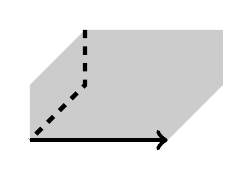
\begin{tikzpicture}[baseline, scale=0.7]
		\fill[gray!40] (0, 1) -- (-1, 0) -- (-1, -1) -- (1.5, -1) --(2.5, 0) -- (2.5, 1)  --cycle;
		\draw[ultra thick, dashed] (0,1) -- (0,0) -- (-1, -1);
		\draw[ultra thick, ->] (-1, -1) -- (1.5, -1);
	\end{tikzpicture} \;\Rightarrow \cdots \Rightarrow\; 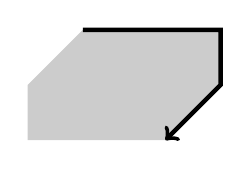
\begin{tikzpicture}[baseline, scale=0.7]
		\fill[gray!40] (-1, 1) -- (1.5, 1) -- (1.5, 0) -- (0.5, -1) -- (-2, -1) -- (-2, 0) --cycle;
		\draw[ultra thick, ->] (-1,1) -- (1.5 , 1) -- (1.5, 0)  -- (0.5, -1);
	\end{tikzpicture} \; =: \beth. \]
	
	回忆到 $\cate{D}(\cdots) \times \cate{D}(\cdots) \to \cate{D}(\cdots)$ 作为右 Kan 延拓是绝对的 (命题 \ref{prop:localization-functor-abs}), 故合成
	\begin{equation*}\begin{gathered}
		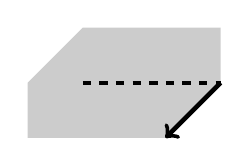
\begin{tikzpicture}[baseline=(O), scale=0.7]
			\fill[gray!40] (-1, 1) -- (1.5, 1) -- (1.5, 0) -- (0.5, -1) -- (-2, -1) -- (-2, 0) --cycle;
			\draw[ultra thick, dashed] (-1,0) -- (1.5, 0);
			\draw[ultra thick, ->] (1.5, 0)  -- (0.5, -1);
			\coordinate (O) at (0, 0);
		\end{tikzpicture}
		\quad \text{是 $\beth$ 沿} \quad
		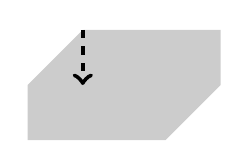
\begin{tikzpicture}[baseline=(O), scale=0.7]
			\fill[gray!40] (-1, 1) -- (1.5, 1) -- (1.5, 0) -- (0.5, -1) -- (-2, -1) -- (-2, 0) --cycle;
			\draw[ultra thick, dashed, ->] (-1, 1) -- (-1, 0);
			\coordinate (O) at (0, 0);
		\end{tikzpicture}
		\quad\text{的右 Kan 延拓.}
	\end{gathered}\end{equation*}
	应用映向 $\beth$ 的态射以及右 Kan 延拓的泛性质 (定义 \ref{def:Kan-extension}) 即得所求之 $\alpha$.
	
	一旦确认了 $\alpha$ 的存在性, 再按证明第一段的方式代入 K-平坦复形, 将一切函子提到上层计算, 即可证 $\alpha$ 为同构.
\end{proof}

今后经常省略这类基于泛性质的论证, 改以解消直接验证.

\begin{corollary}\label{prop:otimesL-Tor}
	\index[sym1]{Tor}
	定义 \ref{def:otimesL} 的函子 $\otimesL[R]$ 在 $A$ 或 $B$ 作为 $\Bbbk$-模平坦的条件下满足典范同构
	\[ \Hm^{-n}\left( X \otimesL[R] Y \right) \simeq \Tor^R_n(X, Y), \quad n \in \Z, \]
	其中 $X$ 是 $(A,R)$-双模, $Y$ 是 $(R,B)$-双模, $\Tor^R_n$ 如定义--命题 \ref{def:Tor-classical}.
\end{corollary}
\begin{proof}
	左式来自命题 \ref{prop:otimesL-enrichment} 的图表按
	\begin{tikzpicture}[xscale=0.3, yscale=0.3, baseline=(O)]
		\draw[->] (0,0) -- (1,0) -- (1, -1);
		\coordinate (O) at (0, -0.7);
	\end{tikzpicture}
	方向的合成, 右式来自按
	\begin{tikzpicture}[xscale=0.3, yscale=0.3, baseline=(O)]
		\draw[->] (0,0) -- (0, -1) -- (1, -1);
		\coordinate (O) at (0, -0.7);
	\end{tikzpicture}
	方向的合成.
\end{proof}

\begin{proposition}[结合约束]\label{prop:otimesL-associativity-constraint}
	\index{daochuzhangliangji!结合约束 (associativity constraint)}
	设 $A$, $B$, $R$, $S$ 为 $\Bbbk$-代数. 考虑以下两个函子
	\begin{gather*}
		\cate{D}((A,R)\dcate{Mod}) \times \cate{D}((R,S)\dcate{Mod}) \times \cate{D}((S,B)\dcate{Mod}) \to \cate{D}((A,B)\dcate{Mod}), \\
		(X, Y, Z) \mapsto (X \otimesL[R] Y) \otimesL[S] Z, \\
		(X, Y, Z) \mapsto X \otimesL[R] (Y \otimesL[S] Z).
	\end{gather*}
	若 $A$ 和 $B$ 作为 $\Bbbk$-模皆平坦, 则有典范同构
	\[ a(X,Y,Z): (X \otimesL[R] Y) \otimesL[S] Z \rightiso X \otimesL[R] (Y \otimesL[S] Z). \]
\end{proposition}
\begin{proof}
	固定 $Y$. 基于命题 \ref{prop:K-flat},	不妨设 $X_R$ 和 ${}_R Z$ 为 K-平坦的. 于是所有 $\otimesL[R]$ 都可以在复形的层次计算, 一切回归张量积的结合约束 \cite[命题 6.5.12]{Li1}.
\end{proof}

在平坦性的前提下, 三个以上的对象按种种次序取 $\otimesL$, 得到的结果依照结合约束两两同构; 这些同构也服从融贯性, 具体可以仿照幺半范畴的五角形公理来表述, 见 \cite[定义 3.1.1]{Li1}. 方法仍是取 K-平坦解消, 化到复形层次去验证. 本书省墨, 仅拈出交换环的特例.

\begin{example}[交换环的 $\otimesL$]\label{eg:commutative-otimesL}
	\index{daochuzhangliangji!交换约束 (commutativity constraint)}
	设 $R$ 为交换环. 在 $\otimesL := \otimesL[R]$ 的定义中将所有环取作 $R$, 特别地 $\Bbbk = R$, 如此则 $(R,R)\dcate{Mod} = R\dcate{Mod}$, 而之前关于平坦性的假设平凡地成立; 于是乎 $\Hm^{-n}(X \otimesL Y) \simeq \Tor^R_n(X,Y)$ 对所有 $R$-模 $X$, $Y$ 皆成立.
	
	这使得 $\cate{D}(R\dcate{Mod})$ 对 $\otimesL$ 成为 \cite[\S 3.1]{Li1} 介绍的幺半范畴, 其幺元由 $R$ 本身给出, 结合约束来自命题 \ref{prop:otimesL-associativity-constraint} 的 $a = (a(X,Y,Z))_{X,Y,Z}$. 留意到 $R$ 是平坦 $R$-模, 因而是 K-平坦的 (命题 \ref{prop:flat-K-flat}), 于是 $R \otimesL (\cdot)$ 和 $(\cdot) \otimesL R$ 皆可在复形层次计算, 由此易证幺半范畴的所有公理. 进一步, $\cate{D}(R\dcate{Mod})$ 还是 \cite[定义 3.3.1]{Li1} 的对称幺半范畴. 对应的辫结构 (或称交换约束) $c(X,Y): X \otimesL Y \rightiso Y \otimesL X$ 来自复形层次的交换约束, 公理同样在复形层次检验; 鉴于命题 \ref{prop:double-cplx-swap}, 全复形的上标对调在此不成问题.
\end{example}

\begin{example}[$\mathrm{Tor}$ 代数]
	承接例 \ref{eg:commutative-otimesL} 的讨论, 设 $R$ 交换. 将 $R$-模构成的复形 $X, Y, Z, W$ 等同于它们在导出范畴中的像. 对所有 $(p,q) \in \Z^2$, 我们有典范态射
	\begin{multline*}
		\Hm^{-p}\left( X \otimesL Y \right) \otimes \Hm^{-q}\left( Z \otimesL W \right) \to \Hm^{-p-q}\left( (X \otimesL Y) \otimesL (Z \otimesL W) \right) \\
		\simeq \Hm^{-p-q}\left( (X \otimesL Z) \otimesL (Y \otimesL W) \right) \to \Hm^{-p-q} \left( (X \otimes Z) \otimesL (Y \otimes W) \right),
	\end{multline*}
	第一段是命题 \ref{prop:bifunctor-cup} 的应用 (取 $F = \otimes$), 第二段用到 $(\cate{D}(R\dcate{Mod}), \otimesL)$ 的结合约束和交换约束, 第三段则来自 $\otimesL$ 作为左导出双函子自带的典范态射
	\[ QX_1 \otimesL QX_2 \to Q(X_1 \otimes X_2), \quad X_1, X_2 \in \Obj(\cate{K}(R\dcate{Mod})), \]
	精确起见, 此处重新标注了局部化函子 $Q: \cate{K}(R\dcate{Mod}) \to \cate{D}(R\dcate{Mod})$.
	\begin{itemize}
		\item 上述三段典范态射的合成, 给出 $\Tor$ 函子的``外乘'':
		\[ \Tor^R_p(X, Y) \otimes \Tor^R_q(Z, W) \to \Tor^R_{p+q}(X \otimes Z, Y \otimes W). \]
		\item 取 $Z=X$, $W=Y$ 为 $R$-代数 (集中在 $0$ 次项), 其乘法给出 $R$-模同态 $X \otimes X \to X$ 和 $Y \otimes Y \to Y$. 外乘再和这些同态作合成, 便有
		\[ \Tor^R_p(X, Y) \otimes \Tor^R_q(X, Y) \to \Tor^R_{p+q}(X,Y), \]
		称为 $\Tor$ 函子的``内乘''. 这使 $\bigoplus_{n \in \Z} \Tor^R_n(X, Y)$ 成为 \cite[定义 7.4.1]{Li1} 所谓的 $\Z$-分次 $R$-代数, 称为 $\Tor$ 代数: 它仅在非负次数项非零, $0$ 次项给出子代数 $\Tor^R_0(X, Y) = X \otimes Y$, 后者的定义可见 \cite[定义 7.3.1]{Li1}. 乘法所需的结合律可以化约到 $\otimesL$ 的结合约束和 $X, Y$ 各自的乘法结合律来验证.
		\index{Tor daishu@$\Tor$-代数 ($\Tor$-algebra)}
		\item 进一步要求 $X$ 和 $Y$ 是交换 $R$-代数. 这时 $\Tor$ 代数还是 \cite[定义 7.4.3]{Li1} 所谓的``反交换'' $\Z$-分次代数\footnote{字面意义稍有误导性, 因为此性质是交换性的自然体现. 称为分次交换更合适, 如例 \ref{eg:graded-module}.}: 对所有 $p, q \in \Z$,
		\[ a \in \Tor^R_p(X, Y), \; b \in \Tor^R_q(X, Y) \implies ab = (-1)^{pq} ba. \]
		既然 $X \otimes X \to X$ 和 $Y \otimes Y \to Y$ 皆交换, 正负号何来? 根源在外乘的定义: 命 $C_1$, $C_2$ 为 $X \otimesL Y$ 的两份副本, 则 $ab$ 和 $ba$ 差一个同构 $C_1 \otimesL C_2 \rightiso C_2 \otimesL C_1$, 即 $\otimesL$ 的交换约束; 若将 $C_1$, $C_2$ 以 K-平坦复形表出, 则此同构在全复形的层次上正是命题 \ref{prop:double-cplx-swap} 定义的同构 $r_{C_1^\bullet \otimes C_2^\bullet}$, 它在 $(p,q)$ 次项给出符号 $(-1)^{pq}$.
	\end{itemize}
\end{example}

回到一般的 $\Bbbk$-代数. 为了探讨 $\otimesL$ 和 $\RHom$ 的伴随关系, 尚需一则引理. 以下用 $\RHom_{(A,B)}$ 表示 $(A,B)\dcate{Mod}$ 的 $\RHom$, 其余种类的双模 (或左模, 右模) 范畴依此类推.

\begin{lemma}\label{prop:RHom-enrichment}
	取定 $\Bbbk$-代数 $A$, $B$, $R$. 假定 $B$ 作为 $\Bbbk$-模平坦, 则从 $(A,B)\dcate{Mod}$ 到 $A\dcate{Mod}$ 的忘却函子保持 K-内射复形, 而且 $\RHom_A$ 典范地升级为函子
	\[ \cate{D}\left((A,R)\dcate{Mod}\right)^{\opp} \times \cate{D}\left((A,B)\dcate{Mod}\right) \to \cate{D}\left((R,B)\dcate{Mod}\right), \]
	换言之, 有典范的 $2$-胞腔图表
	\[\begin{tikzcd}
		\cate{D}\left((A,R)\dcate{Mod}\right)^{\opp} \times \cate{D}\left((A,B)\dcate{Mod}\right) \arrow[r] \arrow[d, "\text{忘却}"'] & \cate{D}\left((R,B)\dcate{Mod}\right) \arrow[d, "\text{忘却}"] \arrow[Rightarrow, ld, "\sim", sloped] \\
		\cate{D}(A\dcate{Mod})^{\opp} \times \cate{D}(A\dcate{Mod}) \arrow[r, "{\RHom_A}"'] & \cate{D}(\cate{Ab}) .
	\end{tikzcd}\]

	同理, 在 $A$ 作为 $\Bbbk$-模平坦的前提下, $\RHom_B$ 也有类似的升级版本.
\end{lemma}
\begin{proof}
	既然 $B$ 是平坦 $\Bbbk$-模, $Y \mapsto {}_A Y$ 有正合的左伴随 $(\cdot) \dotimes{\Bbbk} B$, 故它保持 K-内射复形.
	
	其次, 取 $X \in \Obj(\cate{K}((A, R)\dcate{Mod}))$, $Y \in \Obj(\cate{K}(A, B)\dcate{Mod})$, 使得 $Y$ 为 K-内射的. 根据上一步, $\Hom^\bullet\left( {}_A X, {}_A Y \right)$ 确定 $\RHom_A({}_A X, {}_A Y)$, 但它同时也是 $(R, B)$-双模构成的复形. 这就完成了升级手续.
\end{proof}

\begin{theorem}[$\RHom$ 和 $\otimesL$ 的伴随关系]\label{prop:RHom-otimesL-adjunction}
	\index{RHom hanzi}
	\index{daochuzhangliangji}
	设 $A$, $B$, $R$ 为 $\Bbbk$-代数. 以下 $X$, $Y$, $Z$ 分别表 $\cate{D}((A,R)\dcate{Mod})$, $\cate{D}((R,B)\dcate{Mod})$, $\cate{D}((A,B)\dcate{Mod})$ 的对象. 假设 $B$ 作为 $\Bbbk$-模平坦, 此时存在 $\cate{D}(\Bbbk\dcate{Mod})$ 中的典范同构
	\begin{equation*}
		\RHom_{(A,B)} \left( X \otimesL[R] Y, Z \right) \rightiso \RHom_{(R,B)}\left( Y, \RHom_A \left( {}_A X, {}_A Z \right) \right).
	\end{equation*}

	若假设 $A$ 作为 $\Bbbk$-模平坦, 则存在 $\cate{D}(\Bbbk\dcate{Mod})$ 中的典范同构
	\begin{equation*}
		\RHom_{(A,B)}\left( X \otimesL[R] Y, Z \right) \rightiso \RHom_{(A,R)}\left( X, \RHom_B\left( Y_B , Z_B \right) \right).
	\end{equation*}
\end{theorem}
\begin{proof}
	考虑第一式. 设 $Y$ 是 K-投射的, $Z$ 是 K-内射的. 引理 \ref{prop:K-projective-flat} 确保 ${}_R Y$ 是 K-平坦的, 而引理 \ref{prop:RHom-enrichment} 确保 ${}_A Z$ 仍是 K-内射的. 所示的 $\RHom$ 和 $\otimesL[R]$ 都可以在复形层次来确定. 所求同构因此化约为命题 \ref{prop:tensor-Hom-cplx} 的内容.
\end{proof}

\begin{example}[环变换的伴随关系]\label{eg:change-of-ring-adjunction}
	对于例 \ref{eg:change-of-rings} 的情形 (取 $R \to S$ 为 $\Bbbk$-代数的同态, $A = S$, $B = \Bbbk$ 和 $X = S$), 定理 \ref{prop:RHom-otimesL-adjunction} 的第一式化为典范同构
	\begin{gather*}
		\RHom_S\left( \mathrm{L} {}_{R \to S} P(Y), Z \right) \simeq \RHom_R\left( Y, {}_R Z \right), \\
		Y \in \Obj(\cate{D}(R\dcate{Mod})), \quad Z \in \Obj(\cate{D}(S\dcate{Mod})).
	\end{gather*}
	为此, 唯一待说明的是 $\RHom_S({}_S S, {}_S Z) \simeq {}_R Z$: 这直接来自复形层次的同构
	\[ \Hom^\bullet\left({}_S S, \cdot\right) \simeq {}_R (\cdot) : \cate{C}(S\dcate{Mod}) \to \cate{C}(R\dcate{Mod}). \]
	
	如果进一步要求 $R$ 和 $S$ 皆是交换环, $\Bbbk := R$, 则 $\RHom_S$ (或 $\RHom_R$) 取值在 $\cate{D}(S\dcate{Mod})$ (或 $\cate{D}(R\dcate{Mod})$). 此时的伴随同构进一步改写作 $\cate{D}(R\dcate{Mod})$ 中的典范同构
	\[ {}_R \RHom_S\left( \mathrm{L} {}_{R \to S} P(Y), Z \right) \simeq \RHom_R\left( Y, {}_R Z \right) . \]
	一切都可以通过取 K-内射和 K-投射解消在复形层面来验证. 右模情形自不待言.
\end{example}


\begin{Exercises}
	% Reference: [KS06, Exercise 10.10]
	\item 设 $(\mathcal{D}, T, \mathcal{H})$ 为预三角范畴 (或三角范畴). 按下式定义一族新的三角 $\mathcal{H}^-$:
	\[ [X \xrightarrow{f} Y \xrightarrow{g} Z \xrightarrow{h} TX] \in \mathcal{H} \iff [X \xrightarrow{f} Y \xrightarrow{g} Z \xrightarrow{-h} TX] \in \mathcal{H}^- . \]
	\begin{enumerate}[(i)]
		\item 证明 $(\mathcal{D}, T, \mathcal{H}^-)$ 也是预三角范畴 (或三角范畴).
		\item 证明 $(\mathcal{D}, T, \mathcal{H})$ 和 $(\mathcal{D}, T, \mathcal{H}^-)$ 作为预三角范畴相互等价.
	\end{enumerate}

	\item 设 $(\mathcal{D}, T, \mathcal{H})$ 为预三角范畴. 证明 $\mathcal{D}$ 中的每个单态射 (或满态射) $u: X \to Y$ 都有左逆 (或右逆). 以此说明预三角范畴若是 Abel 范畴, 则必然分裂 (定义 \ref{def:semisimple}).
	
	\begin{hint}
		将单态射 $u$ 置入好三角 $X \xrightarrow{u} Y \xrightarrow{v} Z \xrightarrow{w} TX$. 由 $u \circ T^{-1}w = 0$ 推导 $w = 0$, 再应用命题 \ref{prop:dt-sum-1}.
	\end{hint}

	\item 应用上一道习题, 举出 Abel 范畴 $\mathcal{A}$ 的例子使得 $\cate{K}(\mathcal{A})$ 和 $\cate{D}(\mathcal{A})$ 皆非 Abel 范畴.

	\begin{hint}
		考虑 $\mathcal{A} = \cate{Ab}$ 中的态射 $f: \Z/p^2 \Z \twoheadrightarrow \Z/p \Z$, 其中 $p$ 是素数. 假若 $\cate{K}(\mathcal{A})$ 是 Abel 范畴, 则讨论 $\cate{K}f$ 和 $\Hm^0(\cate{K}f)$ 的满--单分解, 将它们拆成直和项的投影和包含态射, 可推导矛盾.
	\end{hint}

	\item 设 $\mathcal{A}$ 为 Abel 范畴. 证明 $\cate{D}(\mathcal{A})$ 是 Abel 范畴当且仅当 $\mathcal{A}$ 分裂.

	\begin{hint}
		对于``仅当''方向, 将 $\mathcal{A}$ 嵌入 $\cate{D}(\mathcal{A})$ 并应用前几道习题的结果. 至于``当''的方向, 试对分裂之 $\mathcal{A}$ 说明取上同调给出从 $\cate{D}(\mathcal{A})$ 到 $\mathcal{A}^{\Z}$ 的等价.
	\end{hint}

	\item 有此一说: 三角范畴的八面体公理 (TR5) 是 Abel 范畴中的同构定理 $\dfrac{X/Z}{Y/Z} \simeq X/Y$ 的一种替身, 其中 $X \supset Y \supset Z$ (定理 \ref{prop:Abel-cat-isom-thm} (ii)). 试明确其含义.

	\item (预三角范畴的 $\mathrm{K}_0$) 对任意预三角范畴 $(\mathcal{D}, T, \mathcal{H})$, 定义 $\mathrm{K}_0(\mathcal{D})$ 为 $\Obj(\mathcal{D})$ 生成的自由 $\Z$-模对以下关系的商,
	\[ \text{存在好三角}\; X \to Y \to Z \xrightarrow{+1} \implies [X] - [Y] + [Z] = 0, \]
	其中 $[X] \in \mathrm{K}_0(\mathcal{D})$ 代表含 $X \in \Obj(\mathcal{D})$ 的等价类.
	\begin{enumerate}[(i)]
		\item 证明 $[0] = 0$, $[TX] = -[X]$ 和 $[X \oplus Y] = [X] + [Y]$.
		\item 说明任何三角函子 $F: \mathcal{D} \to \mathcal{D}'$ 都诱导典范同态 $\mathrm{K}_0(\mathcal{D}) \to \mathrm{K}_0(\mathcal{D}')$.
		\item 考虑上同调函子 $H: \mathcal{D} \to \mathcal{A}$, 其中 $\mathcal{A}$ 是 Abel 范畴. 设对于所有 $X$ 都有 $|n| \gg_X 0 \implies H(T^n X) = 0$. 请定义自然同态 $\mathrm{K}_0(\mathcal{D}) \to \mathrm{K}_0(\mathcal{A})$.
		
		\begin{hint}
			映 $[X]$ 为 $\sum_n (-1)^n [H(T^n X)]$. 应用引理 \ref{prop:K0-prep} (iv).
		\end{hint}
		\item 考虑特例 $\mathcal{D} := \cate{D}^{\bdd}(\mathcal{A})$. 给出互逆同态
		\[\begin{tikzcd}[row sep=tiny]
			\mathrm{K}_0(\mathcal{A}) \arrow[shift left, r] & \mathrm{K}_0(\cate{D}^{\bdd}(\mathcal{A})) \arrow[shift left, l] \\
			{[A]} \arrow[mapsto, r] & {[A]} \\
			\sum_n (-1)^n {[\Hm^n(X)]} & {[X]} \arrow[mapsto, l]
		\end{tikzcd}\]
		其中 $A \in \Obj(\mathcal{A})$, 也看作集中在 $0$ 次项的复形.
		\begin{hint}
			一个方向明显互逆, 另一个方向则需要复形的截断.
		\end{hint}
	\end{enumerate}
	\index{K0 qun} \index[sym1]{K0}

	\item 设 $X \in \Obj(\cate{D}(\mathcal{A}))$, 证明
	\begin{gather*}
		X \in \cate{D}^{\leq 0}(\mathcal{A}) \iff \forall Z \in \Obj(\cate{D}^{\geq 1}(\mathcal{A})), \; \Hom_{\cate{D}(\mathcal{A})}(X, Z) = 0, \\
		X \in \cate{D}^{\geq 0}(\mathcal{A}) \iff \forall Z \in \Obj(\cate{D}^{\leq -1}(\mathcal{A})), \; \Hom_{\cate{D}(\mathcal{A})}(Z, X) = 0.
	\end{gather*}
	\begin{hint}
		应用命题 \ref{prop:derived-cat-orthogonality} (i) 以及命题 \ref{prop:derived-truncation-adjunction} 的伴随对和好三角. \end{hint}

	\item 在定理 \ref{prop:localization-triangulated-composite} 的情境下, 假设 $F'$ 满足 $F'(\Obj(\mathcal{N}')) \subset \Obj(\mathcal{N}'')$ (设想成某种``正合性''), 则在 $\mathcal{D}$ 有 $F$-内射或 $F$-投射子范畴的前提下, 典范态射
	\[ \mathrm{R}^{\mathcal{N}''}_{\mathcal{N}} (F' F) \to \left( \mathrm{R}^{\mathcal{N}''}_{\mathcal{N}'} F' \right) \left( \mathrm{R}^{\mathcal{N}'}_{\mathcal{N}} F \right) \]
	或
	\[ \left( \mathrm{L}^{\mathcal{N}''}_{\mathcal{N'}} F' \right) \left( \mathrm{L}^{\mathcal{N}'}_{\mathcal{N}} F \right) \to \mathrm{L}^{\mathcal{N}''}_{\mathcal{N}} (F' F) \]
	为同构.
	
	\item 在定理 \ref{prop:localization-triangulated-composite} 的情境下, 说明有函子及其间态射的交换图表 (省略符号 $\mathcal{N}$ 等):
	\[\begin{tikzcd}
		\mathrm{R}(F'' F' F) \arrow[r] \arrow[d] & \mathrm{R}(F'' F') \mathrm{R}F \arrow[d] \\
		\mathrm{R}F'' \mathrm{R}(F'F) \arrow[r] & \mathrm{R}F'' \mathrm{R}F' \mathrm{R}F
	\end{tikzcd} \quad \begin{tikzcd}
		\mathrm{L}(F'' F' F) & \mathrm{L}(F'' F') \mathrm{L}F \arrow[l] \\
		\mathrm{L}F'' \mathrm{L}(F'F) \arrow[u] & \mathrm{L}F'' \mathrm{L}F' \mathrm{L}F \arrow[u] \arrow[l] .
	\end{tikzcd}\]

	\item 对 $F = \Hom$ 明确命题 \ref{prop:bifunctor-cup} 给出的典范态射, 表为 $\Ext^{q-p}(X, Y) \to \Hom\left( \Hm^p(X), \Hm^q(Y) \right)$.

	\item 如将定理 \ref{prop:Yoneda-Ext} 的双射改为以下形式: 从 $n$-扩张 $0 \to Y \to E^1 \to \cdots \to E^n \to X \to 0$ 构造 $t^{-1} b \in \Hom_{\cate{D}(\mathcal{A})}(X, Y[n])$ 如下
	\[\begin{tikzcd}
		X \arrow[d, "b"']\arrow[phantom, r, "" {name=A, yshift=2ex}] & {} & & & X \arrow[d, "\identity"] \\
		W & E^1 \arrow[r] & E^2 \arrow[r] & \cdots \arrow[r] & X \\
		Y[n] \arrow[u, "{t: \text{拟同构}}"] \arrow[phantom, r, "" {name=B, yshift=-2ex}] & Y \arrow[u] & & &
		\arrow[dash, from=A, to=B]
	\end{tikzcd}\]
	由此得到 $t^{-1} b \in \Hom_{\cate{D}(\mathcal{A})}(X, Y[n])$. 证明它和基于 $as^{-1}$ 的原双射相差 $(-1)^n$. 对于 $n=1$ 的特例, 用 $t^{-1} b$ 的版本推导命题 \ref{prop:Ext1-via-ses} 的相应版本 (涉及 $\identity_Y$ 的像).
	
	\begin{hint}
		证明 $ta + (-1)^{n-1} bs: Z \to W$ 典范地零伦. 对于第二部分, 留意命题 \ref{prop:ses-vs-triangle} 中的负号.
	\end{hint}

	\item 设 Abel 范畴 $\mathcal{A}$ 的所有对象 $S, T$ 皆满足 $\Ext^2_{\mathcal{A}}(S,T) = 0$. 证明每个 $X \in \Obj(\cate{D}^{\bdd}(\mathcal{A}))$ 都同构于 $\bigoplus_n \Hm^n(X)[-n]$. 说明 $\mathcal{A} := \Z\dcate{Mod}$ 满足此条件.
	
	\begin{hint}
		不妨设 $X$ 是有界复形. 从 $n \gg 0$ 的情形起步, 对 $2$-扩张 $0 \to \Ker(d^n) \to X^n \xrightarrow{d^n} X^{n+1} \to \Coker(d^n) \to 0$ 应用定理 \ref{prop:Yoneda-Ext} 和命题 \ref{prop:Yoneda-zero}, 在同构意义下逐步修改 $X$ 使得 $d^\bullet = 0$.
	\end{hint}

	\item 证明若 $\mathcal{A}$ 有足够的内射对象, $F: \mathcal{A} \to \mathcal{A}'$ 是左正合加性函子, 而 $\mathrm{R}F$ 的维数有限, 则从三角函子 $\mathrm{R}F$ 诱导的 $\mathrm{K}_0(\mathcal{A}) \simeq \mathrm{K}_0(\cate{D}^{\bdd}(\mathcal{A})) \to \mathrm{K}_0(\cate{D}^{\bdd}(\mathcal{A}')) \simeq \mathrm{K}_0(\mathcal{A}')$ 由下式确定
	\[ [A] \mapsto \sum_n (-1)^n \left[\mathrm{R}^n F(A)\right], \quad A \in \Obj(\mathcal{A}). \]

	\item 设 $R$ 为环, 证明 $\cate{C}(R\dcate{Mod})$ 中的 K-平坦复形的滤过 $\varinjlim$ 仍然 K-平坦.
	
	\item 设 $R$ 为环. 若 $R$-模构成的复形 $P$ 是 K-平坦的, 而且每个 $P^n$ 都是平坦 $R$-模, 则称 $P$ 是强 K-平坦的.
	\begin{enumerate}[(i)]
		\item 证明对于任何 $X \in \Obj(\cate{C}(R\dcate{Mod}))$ 都存在强 K-平坦复形 $P$ 连同拟同构 $P \to X$.
		\begin{hint}
			将 K-内射解消存在性的论证适当地对偶化, 见 \S\ref{sec:K-injectives}.
		\end{hint}
		\item 以 $\mathcal{SF}$ 表示强 K-平坦复形在 $\cate{K}(R\dcate{Mod})$ 中组成的全子范畴. 将范畴 $\cate{D}(R\dcate{Mod})$ 表成 $\mathcal{SF}$ 对拟同构的局部化.
	\end{enumerate}

	\item (P.\ Berthelot, A.\ Ogus) 设 $f$ 为交换环 $R$ 中的非零因子. 对任意 $R$-模 $M$, 记 $M[f] := \{m \in M: fm=0 \}$; 满足 $M[f] = 0$ 的模 $M$ 被称为 $f$-无挠的. 先说明 $f$-无挠的 $M$ 可嵌入为 $M[\frac{1}{f}] = M \dotimes{R} R[\frac{1}{f}]$ 的子模, 故 $f^m M$ 对任何 $m \in \Z$ 都有意义.

	设 $X$ 是由 $f$-无挠 $R$-模构成的复形, 基于上述观察, 定义 $X^\bullet \dotimes{R} R[\frac{1}{f}]$ 的子复形 $\eta_f X$ 为
	\[ (\eta_f X)^n := \left\{ x \in f^n X^n : d_X^n(x) \in f^{n+1} X^{n+1} \right\}, \quad n \in \Z . \]
	\begin{enumerate}[(i)]
		\item 证明逐项乘以 $f$ 给出同构 $\eta_f(X[1]) \rightiso (\eta_f X)[1]$.
		\item 说明若 $f, g \in R$ 皆非零因子, 且每个 $X^n$ 都是 $fg$-无挠的, 则 $\eta_f \eta_g X = \eta_{fg} X$.
		\item 给出典范同构 $\Hm^n(X)/\Hm^n(X)[f] \rightiso \Hm^n(\eta_f X)$; 因此 $\eta_f$ 的效果是矫正 $f$-挠. 由此推导若 $X$, $Y$ 是由 $f$-无挠 $R$-模构成的复形, $\alpha: X \to Y$ 是拟同构, 则它诱导拟同构 $\eta_f(\alpha): \eta_f X \to \eta_f Y$.
		\item 证明 $\eta_f$ 按此诱导加性函子 $\mathrm{L}\eta_f: \cate{D}(R\dcate{Mod}) \to \cate{D}(R\dcate{Mod})$, 使得它拉回上一道习题的 $\mathcal{SF}$ 等于 $\eta_f$.
		\item 说明 $\mathrm{L}\eta_f$ 不是三角函子. 因此它并非定义 \ref{def:Verdier-localization-functor} 下的左导出函子, 尽管它仍是一个右 Kan 延拓.

		\begin{hint}
			取 $R = \Z$ 和 $f = p$ 为素数. 验证 $\mathrm{L}\eta_p(\Z/p\Z) = 0$ 而 $\mathrm{L}\eta_p(\Z/p^2\Z) \simeq \Z/p\Z$.
		\end{hint}
	\end{enumerate}

	\item 承上题, 给出典范态射 $\mathrm{L}\eta_f X \otimesL[R] \mathrm{L}\eta_f Y \to \mathrm{L}\eta_f\left( X \otimesL[R] Y \right)$, 并且说明它在适当意义下对 $X$ 和 $Y$ 是对称的. 实际上, 按照 \cite[注记 3.1.8]{Li1} 的语言, $\mathrm{L}\eta_f$ 对 $\otimesL[R]$ 是右松幺半函子.
\end{Exercises}
